%&preformat-disser
\RequirePackage[l2tabu,orthodox]{nag} % Раскомментировав, можно в логе получать рекомендации относительно правильного использования пакетов и предупреждения об устаревших и нерекомендуемых пакетах
% Формат А4, 14pt (ГОСТ Р 7.0.11-2011, 5.3.6)
\documentclass[a4paper,14pt,oneside,openany]{memoir}

%%%%%%%%%%%%%%%%%%%%%%%%%%%%%%%%%%%%%%%%%%%%%%%%%%%%%%%
%%%% Файл упрощённых настроек шаблона автореферата %%%%
%%%%%%%%%%%%%%%%%%%%%%%%%%%%%%%%%%%%%%%%%%%%%%%%%%%%%%%

%%% Инициализирование переменных, не трогать!  %%%
\newcounter{showperssign}
\newcounter{showsecrsign}
\newcounter{showopplead}
%%%%%%%%%%%%%%%%%%%%%%%%%%%%%%%%%%%%%%%%%%%%%%%%%%%%%%%

%%% Список публикаций %%%
\makeatletter
\@ifundefined{c@usefootcite}{
  \newcounter{usefootcite}
  \setcounter{usefootcite}{0} % 0 --- два списка литературы;
                              % 1 --- список публикаций автора + цитирование
                              %       других работ в сносках
}{}
\makeatother

\makeatletter
\@ifundefined{c@bibgrouped}{
  \newcounter{bibgrouped}
  \setcounter{bibgrouped}{0}  % 0 --- единый список работ автора;
                              % 1 --- сгруппированные работы автора
}{}
\makeatother

%%% Область упрощённого управления оформлением %%%

%% Управление зазором между подрисуночной подписью и основным текстом %%
\setlength{\belowcaptionskip}{10pt plus 20pt minus 2pt}


%% Подпись таблиц %%

% смещение строк подписи после первой
\newcommand{\tabindent}{0cm}

% тип форматирования таблицы
% plain --- название и текст в одной строке
% split --- название и текст в разных строках
\newcommand{\tabformat}{plain}

%%% настройки форматирования таблицы `plain'

% выравнивание по центру подписи, состоящей из одной строки
% true  --- выравнивать
% false --- не выравнивать
\newcommand{\tabsinglecenter}{false}

% выравнивание подписи таблиц
% justified   --- выравнивать как обычный текст
% centering   --- выравнивать по центру
% centerlast  --- выравнивать по центру только последнюю строку
% centerfirst --- выравнивать по центру только первую строку
% raggedleft  --- выравнивать по правому краю
% raggedright --- выравнивать по левому краю
\newcommand{\tabjust}{justified}

% Разделитель записи «Таблица #» и названия таблицы
\newcommand{\tablabelsep}{~\cyrdash\ }

%%% настройки форматирования таблицы `split'

% положение названия таблицы
% \centering   --- выравнивать по центру
% \raggedleft  --- выравнивать по правому краю
% \raggedright --- выравнивать по левому краю
\newcommand{\splitformatlabel}{\raggedleft}

% положение текста подписи
% \centering   --- выравнивать по центру
% \raggedleft  --- выравнивать по правому краю
% \raggedright --- выравнивать по левому краю
\newcommand{\splitformattext}{\raggedright}

%% Подпись рисунков %%
%Разделитель записи «Рисунок #» и названия рисунка
\newcommand{\figlabelsep}{.\ }  % (ГОСТ 2.105, 4.3.1)
                                        % "--- здесь не работает

%Демонстрация подписи диссертанта на автореферате
\setcounter{showperssign}{1}  % 0 --- не показывать;
                              % 1 --- показывать
%Демонстрация подписи учёного секретаря на автореферате
\setcounter{showsecrsign}{1}  % 0 --- не показывать;
                              % 1 --- показывать
%Демонстрация информации об оппонентах и ведущей организации на автореферате
\setcounter{showopplead}{1}   % 0 --- не показывать;
                              % 1 --- показывать

%%% Цвета гиперссылок %%%
% Latex color definitions: http://latexcolor.com/
%\definecolor{linkcolor}{rgb}{0.9,0,0}
%\definecolor{citecolor}{rgb}{0,0.6,0}
%\definecolor{urlcolor}{rgb}{0,0,1}
\definecolor{linkcolor}{rgb}{0,0,0} %black
\definecolor{citecolor}{rgb}{0,0,0} %black
\definecolor{urlcolor}{rgb}{0,0,0} %black
            % общие настройки шаблона
%%% Проверка используемого TeX-движка %%%
\newif\ifxetexorluatex   % определяем новый условный оператор (http://tex.stackexchange.com/a/47579)
\ifxetex
    \xetexorluatextrue
\else
    \ifluatex
        \xetexorluatextrue
    \else
        \xetexorluatexfalse
    \fi
\fi

\newif\ifsynopsis           % Условие, проверяющее, что документ --- автореферат

\usepackage{etoolbox}[2015/08/02]   % Для продвинутой проверки разных условий
\providebool{presentation}

\usepackage{comment}    % Позволяет убирать блоки текста (добавляет
                        % окружение comment и команду \excludecomment)

\usepackage{diagbox}    % Добавляет возможность в качестве разделителя таблицы использовать косую черту

%%% Поля и разметка страницы %%%
\usepackage{pdflscape}  % Для включения альбомных страниц
\usepackage{geometry}   % Для последующего задания полей

%%% Математические пакеты %%%
\usepackage{amsthm,amsmath,amscd}   % Математические дополнения от AMS
\usepackage{amsfonts,amssymb}       % Математические дополнения от AMS
\usepackage{mathtools}              % Добавляет окружение multlined
\usepackage{xfrac}                  % Красивые дроби
\usepackage[
    locale = DE,
    list-separator       = {;\,},
    list-final-separator = {;\,},
    list-pair-separator  = {;\,},
    list-units           = single,
    range-units          = single,
    range-phrase={\text{\ensuremath{-}}},
    % quotient-mode        = fraction, % красивые дроби могут не соответствовать ГОСТ
    fraction-function    = \sfrac,
    separate-uncertainty,
    ]{siunitx}[=v2]                 % Размерности SI
\sisetup{inter-unit-product = \ensuremath{{}\cdot{}}}

% Кириллица в нумерации subequations
% Для правильной работы требуется выполнение сразу после загрузки пакетов
\patchcmd{\subequations}{\def\theequation{\theparentequation\alph{equation}}}
{\def\theequation{\theparentequation\asbuk{equation}}}
{\typeout{subequations patched}}{\typeout{subequations not patched}}

%%%% Установки для размера шрифта 14 pt %%%%
%% Формирование переменных и констант для сравнения (один раз для всех подключаемых файлов)%%
%% должно располагаться до вызова пакета fontspec или polyglossia, потому что они сбивают его работу
\newlength{\curtextsize}
\newlength{\bigtextsize}
\setlength{\bigtextsize}{13.9pt}

\makeatletter
%\show\f@size    % неплохо для отслеживания, но вызывает стопорение процесса,
                 % если документ компилируется без команды  -interaction=nonstopmode
\setlength{\curtextsize}{\f@size pt}
\makeatother

%%% Кодировки и шрифты %%%
\ifxetexorluatex
    \ifpresentation
        \providecommand*\autodot{} % quick fix for polyglossia 1.50
    \fi
    \PassOptionsToPackage{no-math}{fontspec}    % https://tex.stackexchange.com/a/26295/104425
    \usepackage{polyglossia}[2014/05/21]        % Поддержка многоязычности
                                        % (fontspec подгружается автоматически)
\else
   %%% Решение проблемы копирования текста в буфер кракозябрами
    \ifnumequal{\value{usealtfont}}{0}{}{
        \input glyphtounicode.tex
        \input glyphtounicode-cmr.tex %from pdfx package
        \pdfgentounicode=1
    }
    \usepackage{cmap}   % Улучшенный поиск русских слов в полученном pdf-файле
    \ifnumequal{\value{usealtfont}}{2}{}{
        \defaulthyphenchar=127  % Если стоит до fontenc, то переносы
                                % не впишутся в выделяемый текст при
                                % копировании его в буфер обмена
    }
    \usepackage{textcomp}
    \usepackage[T1,T2A]{fontenc}                    % Поддержка русских букв
    \ifnumequal{\value{usealtfont}}{1}{% Используется pscyr, при наличии
        \IfFileExists{pscyr.sty}{\usepackage{pscyr}}{}  % Подключение pscyr
    }{}
    \usepackage[utf8]{inputenc}[2014/04/30]         % Кодировка utf8
    \usepackage[english, russian]{babel}[2014/03/24]% Языки: русский, английский
    \makeatletter\AtBeginDocument{\let\@elt\relax}\makeatother % babel 3.40 fix
    \ifnumequal{\value{usealtfont}}{2}{
        % http://dxdy.ru/post1238763.html#p1238763
        \usepackage[scaled=0.914]{XCharter}[2017/12/19] % Подключение русифицированных шрифтов XCharter
        \usepackage[charter, vvarbb, scaled=1.048]{newtxmath}[2017/12/14]
        \ifpresentation
        \else
            \setDisplayskipStretch{-0.078}
        \fi
    }{}
\fi

%%% Оформление абзацев %%%
\ifpresentation
\else
    \indentafterchapter     % Красная строка после заголовков типа chapter
    \usepackage{indentfirst}
\fi

%%% Цвета %%%
\ifpresentation
\else
    \usepackage[dvipsnames, table, hyperref]{xcolor} % Совместимо с tikz
\fi

%%% Таблицы %%%
\usepackage{longtable,ltcaption} % Длинные таблицы
\usepackage{multirow,makecell}   % Улучшенное форматирование таблиц
\usepackage{tabu, tabulary}      % таблицы с автоматически подбирающейся
                                 % шириной столбцов (tabu обязательно
                                 % до hyperref вызывать)
\makeatletter
%https://github.com/tabu-issues-for-future-maintainer/tabu/issues/26
\@ifpackagelater{longtable}{2020/02/07}{
\def\tabuendlongtrial{%
    \LT@echunk  \global\setbox\LT@gbox \hbox{\unhbox\LT@gbox}\kern\wd\LT@gbox
                \LT@get@widths
}%
}{}
\makeatother

\usepackage{threeparttable}      % автоматический подгон ширины подписи таблицы

%%% Общее форматирование
\usepackage{soulutf8}% Поддержка переносоустойчивых подчёркиваний и зачёркиваний
\usepackage{icomma}  % Запятая в десятичных дробях

%%% Оптимизация расстановки переносов и длины последней строки абзаца
\IfFileExists{impnattypo.sty}{% проверка установленности пакета impnattypo
    \ifluatex
        \ifnumequal{\value{draft}}{1}{% Черновик
            \usepackage[hyphenation, lastparline, nosingleletter, homeoarchy,
            rivers, draft]{impnattypo}
        }{% Чистовик
            \usepackage[hyphenation, lastparline, nosingleletter]{impnattypo}
        }
    \else
        \usepackage[hyphenation, lastparline]{impnattypo}
    \fi
}{}

%% Векторная графика

\usepackage{tikz}                   % Продвинутый пакет векторной графики
\usetikzlibrary{chains}             % Для примера tikz рисунка
\usetikzlibrary{shapes.geometric}   % Для примера tikz рисунка
\usetikzlibrary{shapes.symbols}     % Для примера tikz рисунка
\usetikzlibrary{arrows}             % Для примера tikz рисунка

\usepackage[european,cuteinductors]{circuitikz} % Электрические схемы
\usepackage{pgfplots}                           % Графики
\pgfplotsset{compat=newest}
\usepgfplotslibrary{groupplots,units}
\pgfkeys{/pgf/number format/.cd,use comma,1000 sep={}} % форматирование чисел в графиках

%%% Гиперссылки %%%
\ifxetexorluatex
    \let\CYRDZE\relax
\fi
\usepackage{hyperref}[2012/11/06]

%%% Изображения %%%
\usepackage{graphicx}[2014/04/25]   % Подключаем пакет работы с графикой
\usepackage{caption}                % Подписи рисунков и таблиц
\usepackage{subcaption}             % Подписи подрисунков и подтаблиц
\usepackage{pdfpages}               % Добавление внешних pdf файлов

%%% Счётчики %%%
\usepackage{aliascnt}
\usepackage[figure,table]{totalcount}   % Счётчик рисунков и таблиц
\usepackage{totcount}   % Пакет создания счётчиков на основе последнего номера
                        % подсчитываемого элемента (может требовать дважды
                        % компилировать документ)
\usepackage{totpages}   % Счётчик страниц, совместимый с hyperref (ссылается
                        % на номер последней страницы). Желательно ставить
                        % последним пакетом в преамбуле

%%% Продвинутое управление групповыми ссылками (пока только формулами) %%%
\ifpresentation
\else
    \usepackage[russian]{cleveref} % cleveref имеет сложности со считыванием
    % языка из babel. Такое решение русификации вывода выбрано вместо
    % определения в documentclass из опасности что-то лишнее передать во все
    % остальные пакеты, включая библиографию.

    % Добавление возможности использования пробелов в \labelcref
    % https://tex.stackexchange.com/a/340502/104425
    \usepackage{kvsetkeys}
    \makeatletter
    \let\org@@cref\@cref
    \renewcommand*{\@cref}[2]{%
        \edef\process@me{%
            \noexpand\org@@cref{#1}{\zap@space#2 \@empty}%
        }\process@me
    }
    \makeatother
\fi

\usepackage{placeins} % для \FloatBarrier

\ifnumequal{\value{draft}}{1}{% Черновик
    \usepackage[firstpage]{draftwatermark}
    \SetWatermarkText{DRAFT}
    \SetWatermarkFontSize{14pt}
    \SetWatermarkScale{15}
    \SetWatermarkAngle{45}
}{}

%%% Цитата, не приводимая в автореферате:
% возможно, актуальна только для biblatex
%\newcommand{\citeinsynopsis}[1]{\ifsynopsis\else ~\cite{#1} \fi}

% если текущий процесс запущен библиотекой tikz-external, то прекомпиляция должна быть включена
\ifdefined\tikzexternalrealjob
    \setcounter{imgprecompile}{1}
\fi

\ifnumequal{\value{imgprecompile}}{1}{% Только если у нас включена предкомпиляция
    \usetikzlibrary{external}   % подключение возможности предкомпиляции
    \tikzexternalize[prefix=images/cache/,optimize command away=\includepdf] % activate! % здесь можно указать отдельную папку для скомпилированных файлов
    \ifxetex
        \tikzset{external/up to date check={diff}}
    \fi
}{}
         % Пакеты общие для диссертации и автореферата
\synopsisfalse                      % Этот документ --- не автореферат
\input{Dissertation/dispackages}    % Пакеты для диссертации
\input{Dissertation/userpackages}   % Пакеты для специфических пользовательских задач

%%%%%%%%%%%%%%%%%%%%%%%%%%%%%%%%%%%%%%%%%%%%%%%%%%%%%%
%%%% Файл упрощённых настроек шаблона диссертации %%%%
%%%%%%%%%%%%%%%%%%%%%%%%%%%%%%%%%%%%%%%%%%%%%%%%%%%%%%

%%% Инициализирование переменных, не трогать!  %%%
\newcounter{intvl}
\newcounter{otstup}
\newcounter{contnumeq}
\newcounter{contnumfig}
\newcounter{contnumtab}
\newcounter{pgnum}
\newcounter{chapstyle}
\newcounter{headingdelim}
\newcounter{headingalign}
\newcounter{headingsize}
%%%%%%%%%%%%%%%%%%%%%%%%%%%%%%%%%%%%%%%%%%%%%%%%%%%%%%

%%% Область упрощённого управления оформлением %%%

%% Интервал между заголовками и между заголовком и текстом %%
% Заголовки отделяют от текста сверху и снизу
% тремя интервалами (ГОСТ Р 7.0.11-2011, 5.3.5)
\setcounter{intvl}{3}               % Коэффициент кратности к размеру шрифта

%% Отступы у заголовков в тексте %%
\setcounter{otstup}{0}              % 0 --- без отступа; 1 --- абзацный отступ

%% Нумерация формул, таблиц и рисунков %%
% Нумерация формул
\setcounter{contnumeq}{0}   % 0 --- пораздельно (во введении подряд,
                            %       без номера раздела);
                            % 1 --- сквозная нумерация по всей диссертации
% Нумерация рисунков
\setcounter{contnumfig}{0}  % 0 --- пораздельно (во введении подряд,
                            %       без номера раздела);
                            % 1 --- сквозная нумерация по всей диссертации
% Нумерация таблиц
\setcounter{contnumtab}{1}  % 0 --- пораздельно (во введении подряд,
                            %       без номера раздела);
                            % 1 --- сквозная нумерация по всей диссертации

%% Оглавление %%
\setcounter{pgnum}{1}       % 0 --- номера страниц никак не обозначены;
                            % 1 --- Стр. над номерами страниц (дважды
                            %       компилировать после изменения настройки)
\settocdepth{subsection}    % до какого уровня подразделов выносить в оглавление
\setsecnumdepth{subsection} % до какого уровня нумеровать подразделы


%% Текст и форматирование заголовков %%
\setcounter{chapstyle}{1}     % 0 --- разделы только под номером;
                              % 1 --- разделы с названием "Глава" перед номером
\setcounter{headingdelim}{1}  % 0 --- номер отделен пропуском в 1em или \quad;
                              % 1 --- номера разделов и приложений отделены
                              %       точкой с пробелом, подразделы пропуском
                              %       без точки;
                              % 2 --- номера разделов, подразделов и приложений
                              %       отделены точкой с пробелом.

%% Выравнивание заголовков в тексте %%
\setcounter{headingalign}{0}  % 0 --- по центру;
                              % 1 --- по левому краю

%% Размеры заголовков в тексте %%
\setcounter{headingsize}{0}   % 0 --- по ГОСТ, все всегда 14 пт;
                              % 1 --- пропорционально изменяющийся размер
                              %       в зависимости от базового шрифта

%% Подпись таблиц %%

% Смещение строк подписи после первой строки
\newcommand{\tabindent}{0cm}

% Тип форматирования заголовка таблицы:
% plain --- название и текст в одной строке
% split --- название и текст в разных строках
\newcommand{\tabformat}{plain}

%%% Настройки форматирования таблицы `plain`

% Выравнивание по центру подписи, состоящей из одной строки:
% true  --- выравнивать
% false --- не выравнивать
\newcommand{\tabsinglecenter}{false}

% Выравнивание подписи таблиц:
% justified   --- выравнивать как обычный текст («по ширине»)
% centering   --- выравнивать по центру
% centerlast  --- выравнивать по центру только последнюю строку
% centerfirst --- выравнивать по центру только первую строку (не рекомендуется)
% raggedleft  --- выравнивать по правому краю
% raggedright --- выравнивать по левому краю
\newcommand{\tabjust}{justified}

% Разделитель записи «Таблица #» и названия таблицы
\newcommand{\tablabelsep}{.\ }

%%% Настройки форматирования таблицы `split`

% Положение названия таблицы:
% \centering   --- выравнивать по центру
% \raggedleft  --- выравнивать по правому краю
% \raggedright --- выравнивать по левому краю
\newcommand{\splitformatlabel}{\raggedleft}

% Положение текста подписи:
% \centering   --- выравнивать по центру
% \raggedleft  --- выравнивать по правому краю
% \raggedright --- выравнивать по левому краю
\newcommand{\splitformattext}{\raggedright}

%% Подпись рисунков %%
%Разделитель записи «Рисунок #» и названия рисунка
\newcommand{\figlabelsep}{.\ }  % (ГОСТ 2.105, 4.3.1)
                                        % "--- здесь не работает

%%% Цвета гиперссылок %%%
% Latex color definitions: http://latexcolor.com/
\definecolor{linkcolor}{rgb}{0.9,0,0}
\definecolor{citecolor}{rgb}{0,0.6,0}
\definecolor{urlcolor}{rgb}{0,0,1}
%\definecolor{linkcolor}{rgb}{0,0,0} %black
%\definecolor{citecolor}{rgb}{0,0,0} %black
%\definecolor{urlcolor}{rgb}{0,0,0} %black
      % Упрощённые настройки шаблона

% Новые переменные, которые могут использоваться во всём проекте
% ГОСТ 7.0.11-2011
% 9.2 Оформление текста автореферата диссертации
% 9.2.1 Общая характеристика работы включает в себя следующие основные структурные
% элементы:
% актуальность темы исследования;
\newcommand{\actualityTXT}{Актуальность исследования.}
% степень ее разработанности;
\newcommand{\progressTXT}{Степень разработанности темы.}
% цели и задачи;
\newcommand{\aimTXT}{Целью}
\newcommand{\tasksTXT}{задачи}
% научную новизну;
\newcommand{\noveltyTXT}{Научная новизна:}
% теоретическую и практическую значимость работы;
%\newcommand{\influenceTXT}{Теоретическая и практическая значимость}
% или чаще используют просто
\newcommand{\influenceTXT}{Практическая значимость}
% методологию и методы исследования;
\newcommand{\methodsTXT}{Методы исследования.}
% положения, выносимые на защиту;
\newcommand{\defpositionsTXT}{Основные положения, выносимые на~защиту:}
% степень достоверности и апробацию результатов.
\newcommand{\reliabilityTXT}{Достоверность}
\newcommand{\probationTXT}{Апробация работы}

\newcommand{\contributionTXT}{Личный вклад соискателя.}
\newcommand{\publicationsTXT}{Публикации.}


%%% Заголовки библиографии:

% для автореферата:
\newcommand{\bibtitleauthor}{Основные результаты диссертации отражены в работах}

% для стиля библиографии `\insertbiblioauthorgrouped`
\newcommand{\bibtitleauthorvak}{В изданиях из списка ВАК РФ}
\newcommand{\bibtitleauthorscopus}{В изданиях, входящих в международную базу цитирования Scopus}
\newcommand{\bibtitleauthorwos}{В изданиях, входящих в международную базу цитирования Web of Science}
\newcommand{\bibtitleauthorother}{В прочих изданиях}
\newcommand{\bibtitleauthorconf}{В сборниках трудов конференций}
\newcommand{\bibtitleauthorpatent}{Зарегистрированные патенты}
\newcommand{\bibtitleauthorprogram}{Зарегистрированные программы для ЭВМ}

% для стиля библиографии `\insertbiblioauthorimportant`:
\newcommand{\bibtitleauthorimportant}{Наиболее значимые \protect\MakeLowercase\bibtitleauthor}

% для списка литературы в диссертации и списка чужих работ в автореферате:
\newcommand{\bibtitlefull}{Список литературы} % (ГОСТ Р 7.0.11-2011, 4)
         % Новые переменные, для всего проекта

%%% Основные сведения %%%
\newcommand{\thesisAuthorLastName}{\fixme{Соколов}}
\newcommand{\thesisAuthorOtherNames}{\fixme{Андрей Александрович}}
\newcommand{\thesisAuthorInitials}{\fixme{А.\,А.}}
\newcommand{\thesisAuthor}             % Диссертация, ФИО автора
{%
    \texorpdfstring{% \texorpdfstring takes two arguments and uses the first for (La)TeX and the second for pdf
        \thesisAuthorLastName~\thesisAuthorOtherNames% так будет отображаться на титульном листе или в тексте, где будет использоваться переменная
    }{%
        \thesisAuthorLastName, \thesisAuthorOtherNames% эта запись для свойств pdf-файла. В таком виде, если pdf будет обработан программами для сбора библиографических сведений, будет правильно представлена фамилия.
    }
}
\newcommand{\thesisAuthorShort}        % Диссертация, ФИО автора инициалами
{\thesisAuthorInitials~\thesisAuthorLastName}
%\newcommand{\thesisUdk}                % Диссертация, УДК
%{\fixme{xxx.xxx}}
\newcommand{\thesisTitle}              % Диссертация, название
{\fixme{МАТЕМАТИЧЕСКИЕ МОДЕЛИ НЕЛОКАЛЬНОЙ ТЕРМОУПРУГОСТИ И ИХ ЧИСЛЕННАЯ РЕАЛИЗАЦИЯ}}
\newcommand{\thesisSpecialtyNumber}    % Диссертация, специальность, номер
{\fixme{1.2.2}}
\newcommand{\thesisSpecialtyTitle}     % Диссертация, специальность, название (название взято с сайта ВАК для примера)
{\fixme{Математическое моделирование, численные методы и комплексы программ}}
%% \newcommand{\thesisSpecialtyTwoNumber} % Диссертация, вторая специальность, номер
%% {\fixme{XX.XX.XX}}
%% \newcommand{\thesisSpecialtyTwoTitle}  % Диссертация, вторая специальность, название
%% {\fixme{Теория и~методика физического воспитания, спортивной тренировки,
%% оздоровительной и~адаптивной физической культуры}}
\newcommand{\thesisDegree}             % Диссертация, ученая степень
{\fixme{кандидата физико-математических наук}}
\newcommand{\thesisDegreeShort}        % Диссертация, ученая степень, краткая запись
{\fixme{канд. физ.-мат. наук}}
\newcommand{\thesisCity}               % Диссертация, город написания диссертации
{\fixme{Москва}}
\newcommand{\thesisYear}               % Диссертация, год написания диссертации
{\the\year}
\newcommand{\thesisOrganization}       % Диссертация, организация
{\fixme{МОСКОВСКИЙ ГОСУДАРСТВЕННЫЙ ТЕХНИЧЕСКИЙ УНИВЕРСИТЕТ имени Н. Э. Баумана (национальный исследовательский университет)}}
\newcommand{\thesisOrganizationShort}  % Диссертация, краткое название организации для доклада
{\fixme{МГТУ им. Н.Э. Баумана}}

\newcommand{\thesisInOrganization}     % Диссертация, организация в предложном падеже: Работа выполнена в ...
{\fixme{МОСКОВСКОМ ГОСУДАРСТВЕННОМ ТЕХНИЧЕСКОМ УНИВЕРСИТЕТЕ имени Н.Э.~Баумана}}

%% \newcommand{\supervisorDead}{}           % Рисовать рамку вокруг фамилии
\newcommand{\supervisorFio}              % Научный руководитель, ФИО
{\fixme{Савельева Инга Юрьевна}}
\newcommand{\supervisorRegalia}          % Научный руководитель, регалии
{\fixme{доктор физико-математических наук, профессор}}
\newcommand{\supervisorFioShort}         % Научный руководитель, ФИО
{\fixme{И.\,Ю.~Савельева}}
\newcommand{\supervisorRegaliaShort}     % Научный руководитель, регалии
{\fixme{д.ф.-м.н., проф.}}

%% \newcommand{\supervisorTwoDead}{}        % Рисовать рамку вокруг фамилии
%% \newcommand{\supervisorTwoFio}           % Второй научный руководитель, ФИО
%% {\fixme{Фамилия Имя Отчество}}
%% \newcommand{\supervisorTwoRegalia}       % Второй научный руководитель, регалии
%% {\fixme{уч. степень, уч. звание}}
%% \newcommand{\supervisorTwoFioShort}      % Второй научный руководитель, ФИО
%% {\fixme{И.\,О.~Фамилия}}
%% \newcommand{\supervisorTwoRegaliaShort}  % Второй научный руководитель, регалии
%% {\fixme{уч.~ст.,~уч.~зв.}}

\newcommand{\opponentOneFio}           % Оппонент 1, ФИО
{\fixme{Фамилия Имя Отчество}}
\newcommand{\opponentOneRegalia}       % Оппонент 1, регалии
{\fixme{доктор физико-математических наук, профессор}}
\newcommand{\opponentOneJobPlace}      % Оппонент 1, место работы
{\fixme{Название для места работы}}
\newcommand{\opponentOneJobPost}       % Оппонент 1, должность
{\fixme{старший научный сотрудник}}

\newcommand{\opponentTwoFio}           % Оппонент 2, ФИО
{\fixme{Фамилия Имя Отчество}}
\newcommand{\opponentTwoRegalia}       % Оппонент 2, регалии
{\fixme{кандидат физико-математических наук}}
\newcommand{\opponentTwoJobPlace}      % Оппонент 2, место работы
{\fixme{Основное место работы}}
\newcommand{\opponentTwoJobPost}       % Оппонент 2, должность
{\fixme{старший научный сотрудник}}

%% \newcommand{\opponentThreeFio}         % Оппонент 3, ФИО
%% {\fixme{Фамилия Имя Отчество}}
%% \newcommand{\opponentThreeRegalia}     % Оппонент 3, регалии
%% {\fixme{кандидат физико-математических наук}}
%% \newcommand{\opponentThreeJobPlace}    % Оппонент 3, место работы
%% {\fixme{Основное место работы c длинным длинным длинным длинным названием}}
%% \newcommand{\opponentThreeJobPost}     % Оппонент 3, должность
%% {\fixme{старший научный сотрудник}}

\newcommand{\leadingOrganizationTitle} % Ведущая организация, дополнительные строки. Удалить, чтобы не отображать в автореферате
{\fixme{Федеральное государственное бюджетное образовательное учреждение высшего образования <<Московский государственный университет имени М.В.~Ломоносова>>, механико-математический факультет}}

\newcommand{\defenseDate}              % Защита, дата
{\fixme{<<\underline{~~}>> \underline{~~~~~~} \the\year~года в \underline{~~} часов}}
\newcommand{\defenseCouncilNumber}     % Защита, номер диссертационного совета
{\fixme{Д\,24.2.331.05}}
\newcommand{\defenseCouncilTitle}      % Защита, учреждение диссертационного совета
{\fixme{МГТУ им. Н.Э.~Баумана}}
\newcommand{\defenseCouncilAddress}    % Защита, адрес учреждение диссертационного совета
{\fixme{Москва, 2-я Бауманская ул., д. 5, стр. 1}}
\newcommand{\defenseCouncilPhone}      % Телефон для справок
{\fixme{+7~(0000)~00-00-00}}

\newcommand{\defenseSecretaryFio}      % Секретарь диссертационного совета, ФИО
{\fixme{Аттетков Александр Владимирович}}
\newcommand{\defenseSecretaryRegalia}  % Секретарь диссертационного совета, регалии
{\fixme{кандидат технических наук, доцент}}            % Для сокращений есть ГОСТы, например: ГОСТ Р 7.0.12-2011 + http://base.garant.ru/179724/#block_30000

\newcommand{\synopsisLibrary}          % Автореферат, название библиотеки
{\fixme{www.bmstu.ru}}
\newcommand{\synopsisDate}             % Автореферат, дата рассылки
{\fixme{<<\underline{~~}>> \underline{~~~~~~}} \the\year~года}

% To avoid conflict with beamer class use \providecommand
\providecommand{\keywords}%            % Ключевые слова для метаданных PDF диссертации и автореферата
{}
             % Основные сведения
\input{common/fonts}            % Определение шрифтов (частичное)
%%% Шаблон %%%
\DeclareRobustCommand{\fixme}{\textcolor{black}}  % решаем проблему превращения
                                % названия цвета в результате \MakeUppercase,
                                % http://tex.stackexchange.com/a/187930,
                                % \DeclareRobustCommand protects \fixme
                                % from expanding inside \MakeUppercase
\AtBeginDocument{%
    \setlength{\parindent}{2.5em}                   % Абзацный отступ. Должен быть одинаковым по всему тексту и равен пяти знакам (ГОСТ Р 7.0.11-2011, 5.3.7).
}

%%% Таблицы %%%
\DeclareCaptionLabelSeparator{tabsep}{\tablabelsep} % нумерация таблиц
\DeclareCaptionFormat{split}{\splitformatlabel#1\par\splitformattext#3}

\captionsetup[table]{
        format=\tabformat,                % формат подписи (plain|hang)
        font=normal,                      % нормальные размер, цвет, стиль шрифта
        skip=.0pt,                        % отбивка под подписью
        parskip=.0pt,                     % отбивка между параграфами подписи
        position=above,                   % положение подписи
        justification=\tabjust,           % центровка
        indent=\tabindent,                % смещение строк после первой
        labelsep=tabsep,                  % разделитель
        singlelinecheck=\tabsinglecenter, % не выравнивать по центру, если умещается в одну строку
}

%%% Рисунки %%%
\DeclareCaptionLabelSeparator{figsep}{\figlabelsep} % нумерация рисунков

\captionsetup[figure]{
        format=plain,                     % формат подписи (plain|hang)
        font=normal,                      % нормальные размер, цвет, стиль шрифта
        skip=.0pt,                        % отбивка под подписью
        parskip=.0pt,                     % отбивка между параграфами подписи
        position=below,                   % положение подписи
        singlelinecheck=true,             % выравнивание по центру, если умещается в одну строку
        justification=centerlast,         % центровка
        labelsep=figsep,                  % разделитель
}

%%% Подписи подрисунков %%%
\DeclareCaptionSubType{figure}
\renewcommand\thesubfigure{\asbuk{subfigure}} % нумерация подрисунков
\ifsynopsis
\DeclareCaptionFont{norm}{\fontsize{10pt}{11pt}\selectfont}
\newcommand{\subfigureskip}{2.pt}
\else
\DeclareCaptionFont{norm}{\fontsize{14pt}{16pt}\selectfont}
\newcommand{\subfigureskip}{0.pt}
\fi

\captionsetup[subfloat]{
        labelfont=norm,                 % нормальный размер подписей подрисунков
        textfont=norm,                  % нормальный размер подписей подрисунков
        labelsep=space,                 % разделитель
        labelformat=brace,              % одна скобка справа от номера
        justification=centering,        % центровка
        singlelinecheck=true,           % выравнивание по центру, если умещается в одну строку
        skip=\subfigureskip,            % отбивка над подписью
        parskip=.0pt,                   % отбивка между параграфами подписи
        position=below,                 % положение подписи
}

%%% Настройки ссылок на рисунки, таблицы и др. %%%
% команды \cref...format отвечают за форматирование при помощи команды \cref
% команды \labelcref...format отвечают за форматирование при помощи команды \labelcref

\ifpresentation
\else
    \crefdefaultlabelformat{#2#1#3}

    % Уравнение
    \crefformat{equation}{(#2#1#3)} % одиночная ссылка с приставкой
    \labelcrefformat{equation}{(#2#1#3)} % одиночная ссылка без приставки
    \crefrangeformat{equation}{(#3#1#4) \cyrdash~(#5#2#6)} % диапазон ссылок с приставкой
    \labelcrefrangeformat{equation}{(#3#1#4) \cyrdash~(#5#2#6)} % диапазон ссылок без приставки
    \crefmultiformat{equation}{(#2#1#3)}{ и~(#2#1#3)}{, (#2#1#3)}{ и~(#2#1#3)} % перечисление ссылок с приставкой
    \labelcrefmultiformat{equation}{(#2#1#3)}{ и~(#2#1#3)}{, (#2#1#3)}{ и~(#2#1#3)} % перечисление без приставки

    % Подуравнение
    \crefformat{subequation}{(#2#1#3)} % одиночная ссылка с приставкой
    \labelcrefformat{subequation}{(#2#1#3)} % одиночная ссылка без приставки
    \crefrangeformat{subequation}{(#3#1#4) \cyrdash~(#5#2#6)} % диапазон ссылок с приставкой
    \labelcrefrangeformat{subequation}{(#3#1#4) \cyrdash~(#5#2#6)} % диапазон ссылок без приставки
    \crefmultiformat{subequation}{(#2#1#3)}{ и~(#2#1#3)}{, (#2#1#3)}{ и~(#2#1#3)} % перечисление ссылок с приставкой
    \labelcrefmultiformat{subequation}{(#2#1#3)}{ и~(#2#1#3)}{, (#2#1#3)}{ и~(#2#1#3)} % перечисление без приставки

    % Глава
    \crefformat{chapter}{#2#1#3} % одиночная ссылка с приставкой
    \labelcrefformat{chapter}{#2#1#3} % одиночная ссылка без приставки
    \crefrangeformat{chapter}{#3#1#4 \cyrdash~#5#2#6} % диапазон ссылок с приставкой
    \labelcrefrangeformat{chapter}{#3#1#4 \cyrdash~#5#2#6} % диапазон ссылок без приставки
    \crefmultiformat{chapter}{#2#1#3}{ и~#2#1#3}{, #2#1#3}{ и~#2#1#3} % перечисление ссылок с приставкой
    \labelcrefmultiformat{chapter}{#2#1#3}{ и~#2#1#3}{, #2#1#3}{ и~#2#1#3} % перечисление без приставки

    % Параграф
    \crefformat{section}{#2#1#3} % одиночная ссылка с приставкой
    \labelcrefformat{section}{#2#1#3} % одиночная ссылка без приставки
    \crefrangeformat{section}{#3#1#4 \cyrdash~#5#2#6} % диапазон ссылок с приставкой
    \labelcrefrangeformat{section}{#3#1#4 \cyrdash~#5#2#6} % диапазон ссылок без приставки
    \crefmultiformat{section}{#2#1#3}{ и~#2#1#3}{, #2#1#3}{ и~#2#1#3} % перечисление ссылок с приставкой
    \labelcrefmultiformat{section}{#2#1#3}{ и~#2#1#3}{, #2#1#3}{ и~#2#1#3} % перечисление без приставки

    % Приложение
    \crefformat{appendix}{#2#1#3} % одиночная ссылка с приставкой
    \labelcrefformat{appendix}{#2#1#3} % одиночная ссылка без приставки
    \crefrangeformat{appendix}{#3#1#4 \cyrdash~#5#2#6} % диапазон ссылок с приставкой
    \labelcrefrangeformat{appendix}{#3#1#4 \cyrdash~#5#2#6} % диапазон ссылок без приставки
    \crefmultiformat{appendix}{#2#1#3}{ и~#2#1#3}{, #2#1#3}{ и~#2#1#3} % перечисление ссылок с приставкой
    \labelcrefmultiformat{appendix}{#2#1#3}{ и~#2#1#3}{, #2#1#3}{ и~#2#1#3} % перечисление без приставки

    % Рисунок
    \crefformat{figure}{#2#1#3} % одиночная ссылка с приставкой
    \labelcrefformat{figure}{#2#1#3} % одиночная ссылка без приставки
    \crefrangeformat{figure}{#3#1#4 \cyrdash~#5#2#6} % диапазон ссылок с приставкой
    \labelcrefrangeformat{figure}{#3#1#4 \cyrdash~#5#2#6} % диапазон ссылок без приставки
    \crefmultiformat{figure}{#2#1#3}{ и~#2#1#3}{, #2#1#3}{ и~#2#1#3} % перечисление ссылок с приставкой
    \labelcrefmultiformat{figure}{#2#1#3}{ и~#2#1#3}{, #2#1#3}{ и~#2#1#3} % перечисление без приставки

    % Таблица
    \crefformat{table}{#2#1#3} % одиночная ссылка с приставкой
    \labelcrefformat{table}{#2#1#3} % одиночная ссылка без приставки
    \crefrangeformat{table}{#3#1#4 \cyrdash~#5#2#6} % диапазон ссылок с приставкой
    \labelcrefrangeformat{table}{#3#1#4 \cyrdash~#5#2#6} % диапазон ссылок без приставки
    \crefmultiformat{table}{#2#1#3}{ и~#2#1#3}{, #2#1#3}{ и~#2#1#3} % перечисление ссылок с приставкой
    \labelcrefmultiformat{table}{#2#1#3}{ и~#2#1#3}{, #2#1#3}{ и~#2#1#3} % перечисление без приставки

    % Листинг
    \crefformat{lstlisting}{#2#1#3} % одиночная ссылка с приставкой
    \labelcrefformat{lstlisting}{#2#1#3} % одиночная ссылка без приставки
    \crefrangeformat{lstlisting}{#3#1#4 \cyrdash~#5#2#6} % диапазон ссылок с приставкой
    \labelcrefrangeformat{lstlisting}{#3#1#4 \cyrdash~#5#2#6} % диапазон ссылок без приставки
    \crefmultiformat{lstlisting}{#2#1#3}{ и~#2#1#3}{, #2#1#3}{ и~#2#1#3} % перечисление ссылок с приставкой
    \labelcrefmultiformat{lstlisting}{#2#1#3}{ и~#2#1#3}{, #2#1#3}{ и~#2#1#3} % перечисление без приставки

    % Листинг
    \crefformat{ListingEnv}{#2#1#3} % одиночная ссылка с приставкой
    \labelcrefformat{ListingEnv}{#2#1#3} % одиночная ссылка без приставки
    \crefrangeformat{ListingEnv}{#3#1#4 \cyrdash~#5#2#6} % диапазон ссылок с приставкой
    \labelcrefrangeformat{ListingEnv}{#3#1#4 \cyrdash~#5#2#6} % диапазон ссылок без приставки
    \crefmultiformat{ListingEnv}{#2#1#3}{ и~#2#1#3}{, #2#1#3}{ и~#2#1#3} % перечисление ссылок с приставкой
    \labelcrefmultiformat{ListingEnv}{#2#1#3}{ и~#2#1#3}{, #2#1#3}{ и~#2#1#3} % перечисление без приставки
\fi

%%% Настройки гиперссылок %%%
\ifluatex
    \hypersetup{
        unicode,                % Unicode encoded PDF strings
    }
\fi

\hypersetup{
    linktocpage=true,           % ссылки с номера страницы в оглавлении, списке таблиц и списке рисунков
%    linktoc=all,                % both the section and page part are links
%    pdfpagelabels=false,        % set PDF page labels (true|false)
    plainpages=false,           % Forces page anchors to be named by the Arabic form  of the page number, rather than the formatted form
    colorlinks,                 % ссылки отображаются раскрашенным текстом, а не раскрашенным прямоугольником, вокруг текста
    linkcolor={linkcolor},      % цвет ссылок типа ref, eqref и подобных
    citecolor={citecolor},      % цвет ссылок-цитат
    urlcolor={urlcolor},        % цвет гиперссылок
%    hidelinks,                  % Hide links (removing color and border)
    pdftitle={\thesisTitle},    % Заголовок
    pdfauthor={\thesisAuthor},  % Автор
    pdfsubject={\thesisSpecialtyNumber\ \thesisSpecialtyTitle},      % Тема
%    pdfcreator={Создатель},     % Создатель, Приложение
%    pdfproducer={Производитель},% Производитель, Производитель PDF
    pdfkeywords={\keywords},    % Ключевые слова
    pdflang={ru},
}
\ifnumequal{\value{draft}}{1}{% Черновик
    \hypersetup{
        draft,
    }
}{}

%%% Списки %%%
% Используем короткое тире (endash) для ненумерованных списков (ГОСТ 2.105-95, пункт 4.1.7, требует дефиса, но так лучше смотрится)
\renewcommand{\labelitemi}{\normalfont\bfseries{--}}

% Перечисление строчными буквами латинского алфавита (ГОСТ 2.105-95, 4.1.7)
%\renewcommand{\theenumi}{\alph{enumi}}
%\renewcommand{\labelenumi}{\theenumi)}

% Перечисление строчными буквами русского алфавита (ГОСТ 2.105-95, 4.1.7)
\makeatletter
\AddEnumerateCounter{\asbuk}{\russian@alph}{щ}      % Управляем списками/перечислениями через пакет enumitem, а он 'не знает' про asbuk, потому 'учим' его
\makeatother
%\renewcommand{\theenumi}{\asbuk{enumi}} %первый уровень нумерации
%\renewcommand{\labelenumi}{\theenumi)} %первый уровень нумерации
\renewcommand{\theenumii}{\asbuk{enumii}} %второй уровень нумерации
\renewcommand{\labelenumii}{\theenumii)} %второй уровень нумерации
\renewcommand{\theenumiii}{\arabic{enumiii}} %третий уровень нумерации
\renewcommand{\labelenumiii}{\theenumiii)} %третий уровень нумерации

\setlist{nosep,%                                    % Единый стиль для всех списков (пакет enumitem), без дополнительных интервалов.
    labelindent=\parindent,leftmargin=*%            % Каждый пункт, подпункт и перечисление записывают с абзацного отступа (ГОСТ 2.105-95, 4.1.8)
}

%%% Правильная нумерация приложений, рисунков и формул %%%
%% По ГОСТ 2.105, п. 4.3.8 Приложения обозначают заглавными буквами русского алфавита,
%% начиная с А, за исключением букв Ё, З, Й, О, Ч, Ь, Ы, Ъ.
%% Здесь также переделаны все нумерации русскими буквами.
\ifxetexorluatex
    \makeatletter
    \def\russian@Alph#1{\ifcase#1\or
       А\or Б\or В\or Г\or Д\or Е\or Ж\or
       И\or К\or Л\or М\or Н\or
       П\or Р\or С\or Т\or У\or Ф\or Х\or
       Ц\or Ш\or Щ\or Э\or Ю\or Я\else\xpg@ill@value{#1}{russian@Alph}\fi}
    \def\russian@alph#1{\ifcase#1\or
       а\or б\or в\or г\or д\or е\or ж\or
       и\or к\or л\or м\or н\or
       п\or р\or с\or т\or у\or ф\or х\or
       ц\or ш\or щ\or э\or ю\or я\else\xpg@ill@value{#1}{russian@alph}\fi}
    \def\cyr@Alph#1{\ifcase#1\or
        А\or Б\or В\or Г\or Д\or Е\or Ж\or
        И\or К\or Л\or М\or Н\or
        П\or Р\or С\or Т\or У\or Ф\or Х\or
        Ц\or Ш\or Щ\or Э\or Ю\or Я\else\xpg@ill@value{#1}{cyr@Alph}\fi}
    \def\cyr@alph#1{\ifcase#1\or
        а\or б\or в\or г\or д\or е\or ж\or
        и\or к\or л\or м\or н\or
        п\or р\or с\or т\or у\or ф\or х\or
        ц\or ш\or щ\or э\or ю\or я\else\xpg@ill@value{#1}{cyr@alph}\fi}
    \makeatother
\else
    \makeatletter
    \if@uni@ode
      \def\russian@Alph#1{\ifcase#1\or
        А\or Б\or В\or Г\or Д\or Е\or Ж\or
        И\or К\or Л\or М\or Н\or
        П\or Р\or С\or Т\or У\or Ф\or Х\or
        Ц\or Ш\or Щ\or Э\or Ю\or Я\else\@ctrerr\fi}
    \else
      \def\russian@Alph#1{\ifcase#1\or
        \CYRA\or\CYRB\or\CYRV\or\CYRG\or\CYRD\or\CYRE\or\CYRZH\or
        \CYRI\or\CYRK\or\CYRL\or\CYRM\or\CYRN\or
        \CYRP\or\CYRR\or\CYRS\or\CYRT\or\CYRU\or\CYRF\or\CYRH\or
        \CYRC\or\CYRSH\or\CYRSHCH\or\CYREREV\or\CYRYU\or
        \CYRYA\else\@ctrerr\fi}
    \fi
    \if@uni@ode
      \def\russian@alph#1{\ifcase#1\or
        а\or б\or в\or г\or д\or е\or ж\or
        и\or к\or л\or м\or н\or
        п\or р\or с\or т\or у\or ф\or х\or
        ц\or ш\or щ\or э\or ю\or я\else\@ctrerr\fi}
    \else
      \def\russian@alph#1{\ifcase#1\or
        \cyra\or\cyrb\or\cyrv\or\cyrg\or\cyrd\or\cyre\or\cyrzh\or
        \cyri\or\cyrk\or\cyrl\or\cyrm\or\cyrn\or
        \cyrp\or\cyrr\or\cyrs\or\cyrt\or\cyru\or\cyrf\or\cyrh\or
        \cyrc\or\cyrsh\or\cyrshch\or\cyrerev\or\cyryu\or
        \cyrya\else\@ctrerr\fi}
    \fi
    \makeatother
\fi


%%http://www.linux.org.ru/forum/general/6993203#comment-6994589 (используется totcount)
\makeatletter
\def\formtotal#1#2#3#4#5{%
    \newcount\@c
    \@c\totvalue{#1}\relax
    \newcount\@last
    \newcount\@pnul
    \@last\@c\relax
    \divide\@last 10
    \@pnul\@last\relax
    \divide\@pnul 10
    \multiply\@pnul-10
    \advance\@pnul\@last
    \multiply\@last-10
    \advance\@last\@c
    #2%
    \ifnum\@pnul=1#5\else%
    \ifcase\@last#5\or#3\or#4\or#4\or#4\else#5\fi
    \fi
}
\makeatother

\newcommand{\formbytotal}[5]{\total{#1}~\formtotal{#1}{#2}{#3}{#4}{#5}}

%%% Команды рецензирования %%%
\ifboolexpr{ (test {\ifnumequal{\value{draft}}{1}}) or (test {\ifnumequal{\value{showmarkup}}{1}})}{
        \newrobustcmd{\todo}[1]{\textcolor{black}{#1}}
        \newrobustcmd{\note}[2][]{\ifstrempty{#1}{#2}{\textcolor{#1}{#2}}}
        \newenvironment{commentbox}[1][]%
        {\ifstrempty{#1}{}{\color{#1}}}%
        {}
}{
        \newrobustcmd{\todo}[1]{}
        \newrobustcmd{\note}[2][]{}
        \excludecomment{commentbox}
}
           % Стили общие для диссертации и автореферата
%%% Переопределение именований, если иначе не сработает %%%
%\gappto\captionsrussian{
%    \renewcommand{\chaptername}{Глава}
%    \renewcommand{\appendixname}{Приложение} % (ГОСТ Р 7.0.11-2011, 5.7)
%}

%%% Изображения %%%
\graphicspath{{images/}{Dissertation/images/}}         % Пути к изображениям

%%% Интервалы %%%
%% По ГОСТ Р 7.0.11-2011, пункту 5.3.6 требуется полуторный интервал
%% Реализация средствами класса (на основе setspace) ближе к типографской классике.
%% И правит сразу и в таблицах (если со звёздочкой)
%\DoubleSpacing*     % Двойной интервал
\OnehalfSpacing*    % Полуторный интервал
%\setSpacing{1.42}   % Полуторный интервал, подобный Ворду (возможно, стоит включать вместе с предыдущей строкой)

%%% Макет страницы %%%
% Выставляем значения полей (ГОСТ 7.0.11-2011, 5.3.7)
\geometry{a4paper, top=2cm, bottom=2cm, left=2.5cm, right=1cm, nofoot, nomarginpar} %, heightrounded, showframe
\setlength{\topskip}{0pt}   %размер дополнительного верхнего поля
\setlength{\footskip}{12.3pt} % снимет warning, согласно https://tex.stackexchange.com/a/334346

%%% Выравнивание и переносы %%%
%% http://tex.stackexchange.com/questions/241343/what-is-the-meaning-of-fussy-sloppy-emergencystretch-tolerance-hbadness
%% http://www.latex-community.org/forum/viewtopic.php?p=70342#p70342
\tolerance 1414
\hbadness 1414
\emergencystretch 1.5em % В случае проблем регулировать в первую очередь
\hfuzz 0.3pt
\vfuzz \hfuzz
%\raggedbottom
%\sloppy                 % Избавляемся от переполнений
\clubpenalty=10000      % Запрещаем разрыв страницы после первой строки абзаца
\widowpenalty=10000     % Запрещаем разрыв страницы после последней строки абзаца
\brokenpenalty=4991     % Ограничение на разрыв страницы, если строка заканчивается переносом

%%% Блок управления параметрами для выравнивания заголовков в тексте %%%
\newlength{\otstuplen}
\setlength{\otstuplen}{\theotstup\parindent}
\ifnumequal{\value{headingalign}}{0}{% выравнивание заголовков в тексте
    \newcommand{\hdngalign}{\centering}                % по центру
    \newcommand{\hdngaligni}{}% по центру
    \setlength{\otstuplen}{0pt}
}{%
    \newcommand{\hdngalign}{}                 % по левому краю
    \newcommand{\hdngaligni}{\hspace{\otstuplen}}      % по левому краю
} % В обоих случаях вроде бы без переноса, как и надо (ГОСТ Р 7.0.11-2011, 5.3.5)

%%% Оглавление %%%
\renewcommand{\cftchapterdotsep}{\cftdotsep}                % отбивка точками до номера страницы начала главы/раздела

%% Переносить слова в заголовке не допускается (ГОСТ Р 7.0.11-2011, 5.3.5). Заголовки в оглавлении должны точно повторять заголовки в тексте (ГОСТ Р 7.0.11-2011, 5.2.3). Прямого указания на запрет переносов в оглавлении нет, но по той же логике невнесения искажений в смысл, лучше в оглавлении не переносить:
\setrmarg{2.55em plus1fil}                             %To have the (sectional) titles in the ToC, etc., typeset ragged right with no hyphenation
\renewcommand{\cftchapterpagefont}{\normalfont}        % нежирные номера страниц у глав в оглавлении
\renewcommand{\cftchapterleader}{\cftdotfill{\cftchapterdotsep}}% нежирные точки до номеров страниц у глав в оглавлении
%\renewcommand{\cftchapterfont}{}                       % нежирные названия глав в оглавлении

\ifnumgreater{\value{headingdelim}}{0}{%
    \renewcommand\cftchapteraftersnum{.\space}       % добавляет точку с пробелом после номера раздела в оглавлении
}{}
\ifnumgreater{\value{headingdelim}}{1}{%
    \renewcommand\cftsectionaftersnum{.\space}       % добавляет точку с пробелом после номера подраздела в оглавлении
    \renewcommand\cftsubsectionaftersnum{.\space}    % добавляет точку с пробелом после номера подподраздела в оглавлении
    \renewcommand\cftsubsubsectionaftersnum{.\space} % добавляет точку с пробелом после номера подподподраздела в оглавлении
    \AfterEndPreamble{% без этого polyglossia сама всё переопределяет
        \setsecnumformat{\csname the#1\endcsname.\space}
    }
}{%
    \renewcommand\cftsectionaftersnum{.\quad}       % добавляет точку с пробелом после номера подраздела в оглавлении
    \renewcommand\cftsubsectionaftersnum{.\quad}    % добавляет точку с пробелом после номера подподраздела в оглавлении
    \renewcommand\cftsubsubsectionaftersnum{.\quad} % добавляет точку с пробелом после номера подподподраздела в оглавлении
    \AfterEndPreamble{% без этого polyglossia сама всё переопределяет
        \setsecnumformat{\csname the#1\endcsname.\quad}
    }
}

\renewcommand*{\cftappendixname}{\appendixname\space} % Слово Приложение в оглавлении

%%% Колонтитулы %%%
% Порядковый номер страницы печатают на середине верхнего поля страницы (ГОСТ Р 7.0.11-2011, 5.3.8)
\makeevenhead{plain}{}{\rmfamily\thepage}{}
\makeoddhead{plain}{}{\rmfamily\thepage}{}
\makeevenfoot{plain}{}{}{}
\makeoddfoot{plain}{}{}{}
\pagestyle{plain}

%%% добавить Стр. над номерами страниц в оглавлении
%%% http://tex.stackexchange.com/a/306950
\newif\ifendTOC

\newcommand*{\tocheader}{
\ifnumequal{\value{pgnum}}{1}{%
    \ifendTOC\else\hbox to \linewidth%
      {\noindent{}~\hfill{Стр.}}\par%
      \ifnumless{\value{page}}{3}{}{%
        \vspace{0.5\onelineskip}
      }
      \afterpage{\tocheader}
    \fi%
}{}%
}%

%%% Оформление заголовков глав, разделов, подразделов %%%
%% Работа должна быть выполнена ... размером шрифта 12-14 пунктов (ГОСТ Р 7.0.11-2011, 5.3.8). То есть не должно быть надписей шрифтом более 14. Так и поставим.
%% Эти установки будут давать одинаковый результат независимо от выбора базовым шрифтом 12 пт или 14 пт
\newcommand{\basegostsectionfont}{\fontsize{14pt}{16pt}\selectfont\bfseries}

\makechapterstyle{thesisgost}{%
    \chapterstyle{default}
    \setlength{\beforechapskip}{0pt}
    \setlength{\midchapskip}{0pt}
    \setlength{\afterchapskip}{\theintvl\curtextsize}
    \renewcommand*{\chapnamefont}{\basegostsectionfont}
    \renewcommand*{\chapnumfont}{\basegostsectionfont}
    \renewcommand*{\chaptitlefont}{\basegostsectionfont}
    \renewcommand*{\chapterheadstart}{}
    \ifnumgreater{\value{headingdelim}}{0}{%
        \renewcommand*{\afterchapternum}{.\space}   % добавляет точку с пробелом после номера раздела
    }{%
        \renewcommand*{\afterchapternum}{\quad}     % добавляет \quad после номера раздела
    }
    \renewcommand*{\printchapternum}{\hdngaligni\hdngalign\chapnumfont \thechapter}
    \renewcommand*{\printchaptername}{}
    \renewcommand*{\printchapternonum}{\hdngaligni\hdngalign}
}

\makeatletter
\makechapterstyle{thesisgostchapname}{%
    \chapterstyle{thesisgost}
    \renewcommand*{\printchapternum}{\chapnumfont \thechapter}
    \renewcommand*{\printchaptername}{\hdngaligni\hdngalign\chapnamefont \@chapapp} %
}
\makeatother

\chapterstyle{thesisgost}

\setsecheadstyle{\basegostsectionfont\hdngalign}
\setsecindent{\otstuplen}

\setsubsecheadstyle{\basegostsectionfont\hdngalign}
\setsubsecindent{\otstuplen}

\setsubsubsecheadstyle{\basegostsectionfont\hdngalign}
\setsubsubsecindent{\otstuplen}

\sethangfrom{\noindent #1} %все заголовки подразделов центрируются с учетом номера, как block

\ifnumequal{\value{chapstyle}}{1}{%
    \chapterstyle{thesisgostchapname}
    \renewcommand*{\cftchaptername}{\chaptername\space} % будет вписано слово Глава перед каждым номером раздела в оглавлении
}{}%

%%% Интервалы между заголовками
\setbeforesecskip{\theintvl\curtextsize}% Заголовки отделяют от текста сверху и снизу тремя интервалами (ГОСТ Р 7.0.11-2011, 5.3.5).
\setaftersecskip{\theintvl\curtextsize}
\setbeforesubsecskip{\theintvl\curtextsize}
\setaftersubsecskip{\theintvl\curtextsize}
\setbeforesubsubsecskip{\theintvl\curtextsize}
\setaftersubsubsecskip{\theintvl\curtextsize}

%%% Вертикальные интервалы глав (\chapter) в оглавлении как и у заголовков
% раскомментировать следующие 2
% \setlength{\cftbeforechapterskip}{0pt plus 0pt}   % ИЛИ эти 2 строки из учебника
% \renewcommand*{\insertchapterspace}{}
% или эту
% \renewcommand*{\cftbeforechapterskip}{0em}


%%% Блок дополнительного управления размерами заголовков
\ifnumequal{\value{headingsize}}{1}{% Пропорциональные заголовки и базовый шрифт 14 пт
    \renewcommand{\basegostsectionfont}{\large\bfseries}
    \renewcommand*{\chapnamefont}{\Large\bfseries}
    \renewcommand*{\chapnumfont}{\Large\bfseries}
    \renewcommand*{\chaptitlefont}{\Large\bfseries}
}{}

%%% Счётчики %%%

%% Упрощённые настройки шаблона диссертации: нумерация формул, таблиц, рисунков
\ifnumequal{\value{contnumeq}}{1}{%
    \counterwithout{equation}{chapter} % Убираем связанность номера формулы с номером главы/раздела
}{}
\ifnumequal{\value{contnumfig}}{1}{%
    \counterwithout{figure}{chapter}   % Убираем связанность номера рисунка с номером главы/раздела
}{}
\ifnumequal{\value{contnumtab}}{1}{%
    \counterwithout{table}{chapter}    % Убираем связанность номера таблицы с номером главы/раздела
}{}

\AfterEndPreamble{
%% регистрируем счётчики в системе totcounter
    \regtotcounter{totalcount@figure}
    \regtotcounter{totalcount@table}       % Если иным способом поставить в преамбуле то ошибка в числе таблиц
    \regtotcounter{TotPages}               % Если иным способом поставить в преамбуле то ошибка в числе страниц
    \newtotcounter{totalappendix}
    \newtotcounter{totalchapter}
}
  % Стили для диссертации
% для вертикального центрирования ячеек в tabulary
\def\zz{\ifx\[$\else\aftergroup\zzz\fi}
%$ \] % <-- чиним подсветку синтаксиса в некоторых редакторах
\def\zzz{\setbox0\lastbox
\dimen0\dimexpr\extrarowheight + \ht0-\dp0\relax
\setbox0\hbox{\raise-.5\dimen0\box0}%
\ht0=\dimexpr\ht0+\extrarowheight\relax
\dp0=\dimexpr\dp0+\extrarowheight\relax
\box0
}

\lstdefinelanguage{Renhanced}%
{keywords={abbreviate,abline,abs,acos,acosh,action,add1,add,%
        aggregate,alias,Alias,alist,all,anova,any,aov,aperm,append,apply,%
        approx,approxfun,apropos,Arg,args,array,arrows,as,asin,asinh,%
        atan,atan2,atanh,attach,attr,attributes,autoload,autoloader,ave,%
        axis,backsolve,barplot,basename,besselI,besselJ,besselK,besselY,%
        beta,binomial,body,box,boxplot,break,browser,bug,builtins,bxp,by,%
        c,C,call,Call,case,cat,category,cbind,ceiling,character,char,%
        charmatch,check,chol,chol2inv,choose,chull,class,close,cm,codes,%
        coef,coefficients,co,col,colnames,colors,colours,commandArgs,%
        comment,complete,complex,conflicts,Conj,contents,contour,%
        contrasts,contr,control,helmert,contrib,convolve,cooks,coords,%
        distance,coplot,cor,cos,cosh,count,fields,cov,covratio,wt,CRAN,%
        create,crossprod,cummax,cummin,cumprod,cumsum,curve,cut,cycle,D,%
        data,dataentry,date,dbeta,dbinom,dcauchy,dchisq,de,debug,%
        debugger,Defunct,default,delay,delete,deltat,demo,de,density,%
        deparse,dependencies,Deprecated,deriv,description,detach,%
        dev2bitmap,dev,cur,deviance,off,prev,,dexp,df,dfbetas,dffits,%
        dgamma,dgeom,dget,dhyper,diag,diff,digamma,dim,dimnames,dir,%
        dirname,dlnorm,dlogis,dnbinom,dnchisq,dnorm,do,dotplot,double,%
        download,dpois,dput,drop,drop1,dsignrank,dt,dummy,dump,dunif,%
        duplicated,dweibull,dwilcox,dyn,edit,eff,effects,eigen,else,%
        emacs,end,environment,env,erase,eval,equal,evalq,example,exists,%
        exit,exp,expand,expression,External,extract,extractAIC,factor,%
        fail,family,fft,file,filled,find,fitted,fivenum,fix,floor,for,%
        For,formals,format,formatC,formula,Fortran,forwardsolve,frame,%
        frequency,ftable,ftable2table,function,gamma,Gamma,gammaCody,%
        gaussian,gc,gcinfo,gctorture,get,getenv,geterrmessage,getOption,%
        getwd,gl,glm,globalenv,gnome,GNOME,graphics,gray,grep,grey,grid,%
        gsub,hasTsp,hat,heat,help,hist,home,hsv,httpclient,I,identify,if,%
        ifelse,Im,image,\%in\%,index,influence,measures,inherits,install,%
        installed,integer,interaction,interactive,Internal,intersect,%
        inverse,invisible,IQR,is,jitter,kappa,kronecker,labels,lapply,%
        layout,lbeta,lchoose,lcm,legend,length,levels,lgamma,library,%
        licence,license,lines,list,lm,load,local,locator,log,log10,log1p,%
        log2,logical,loglin,lower,lowess,ls,lsfit,lsf,ls,machine,Machine,%
        mad,mahalanobis,make,link,margin,match,Math,matlines,mat,matplot,%
        matpoints,matrix,max,mean,median,memory,menu,merge,methods,min,%
        missing,Mod,mode,model,response,mosaicplot,mtext,mvfft,na,nan,%
        names,omit,nargs,nchar,ncol,NCOL,new,next,NextMethod,nextn,%
        nlevels,nlm,noquote,NotYetImplemented,NotYetUsed,nrow,NROW,null,%
        numeric,\%o\%,objects,offset,old,on,Ops,optim,optimise,optimize,%
        options,or,order,ordered,outer,package,packages,page,pairlist,%
        pairs,palette,panel,par,parent,parse,paste,path,pbeta,pbinom,%
        pcauchy,pchisq,pentagamma,persp,pexp,pf,pgamma,pgeom,phyper,pico,%
        pictex,piechart,Platform,plnorm,plogis,plot,pmatch,pmax,pmin,%
        pnbinom,pnchisq,pnorm,points,poisson,poly,polygon,polyroot,pos,%
        postscript,power,ppoints,ppois,predict,preplot,pretty,Primitive,%
        print,prmatrix,proc,prod,profile,proj,prompt,prop,provide,%
        psignrank,ps,pt,ptukey,punif,pweibull,pwilcox,q,qbeta,qbinom,%
        qcauchy,qchisq,qexp,qf,qgamma,qgeom,qhyper,qlnorm,qlogis,qnbinom,%
        qnchisq,qnorm,qpois,qqline,qqnorm,qqplot,qr,Q,qty,qy,qsignrank,%
        qt,qtukey,quantile,quasi,quit,qunif,quote,qweibull,qwilcox,%
        rainbow,range,rank,rbeta,rbind,rbinom,rcauchy,rchisq,Re,read,csv,%
        csv2,fwf,readline,socket,real,Recall,rect,reformulate,regexpr,%
        relevel,remove,rep,repeat,replace,replications,report,require,%
        resid,residuals,restart,return,rev,rexp,rf,rgamma,rgb,rgeom,R,%
        rhyper,rle,rlnorm,rlogis,rm,rnbinom,RNGkind,rnorm,round,row,%
        rownames,rowsum,rpois,rsignrank,rstandard,rstudent,rt,rug,runif,%
        rweibull,rwilcox,sample,sapply,save,scale,scan,scan,screen,sd,se,%
        search,searchpaths,segments,seq,sequence,setdiff,setequal,set,%
        setwd,show,sign,signif,sin,single,sinh,sink,solve,sort,source,%
        spline,splinefun,split,sqrt,stars,start,stat,stem,step,stop,%
        storage,strstrheight,stripplot,strsplit,structure,strwidth,sub,%
        subset,substitute,substr,substring,sum,summary,sunflowerplot,svd,%
        sweep,switch,symbol,symbols,symnum,sys,status,system,t,table,%
        tabulate,tan,tanh,tapply,tempfile,terms,terrain,tetragamma,text,%
        time,title,topo,trace,traceback,transform,tri,trigamma,trunc,try,%
        ts,tsp,typeof,unclass,undebug,undoc,union,unique,uniroot,unix,%
        unlink,unlist,unname,untrace,update,upper,url,UseMethod,var,%
        variable,vector,Version,vi,warning,warnings,weighted,weights,%
        which,while,window,write,\%x\%,x11,X11,xedit,xemacs,xinch,xor,%
        xpdrows,xy,xyinch,yinch,zapsmall,zip},%
    otherkeywords={!,!=,~,$,*,\%,\&,\%/\%,\%*\%,\%\%,<-,<<-},%$
    alsoother={._$},%$
    sensitive,%
    morecomment=[l]\#,%
    morestring=[d]",%
    morestring=[d]'% 2001 Robert Denham
}%

%решаем проблему с кириллицей в комментариях (в pdflatex) https://tex.stackexchange.com/a/103712
\lstset{extendedchars=true,keepspaces=true,literate={Ö}{{\"O}}1
    {Ä}{{\"A}}1
    {Ü}{{\"U}}1
    {ß}{{\ss}}1
    {ü}{{\"u}}1
    {ä}{{\"a}}1
    {ö}{{\"o}}1
    {~}{{\textasciitilde}}1
    {а}{{\selectfont\char224}}1
    {б}{{\selectfont\char225}}1
    {в}{{\selectfont\char226}}1
    {г}{{\selectfont\char227}}1
    {д}{{\selectfont\char228}}1
    {е}{{\selectfont\char229}}1
    {ё}{{\"e}}1
    {ж}{{\selectfont\char230}}1
    {з}{{\selectfont\char231}}1
    {и}{{\selectfont\char232}}1
    {й}{{\selectfont\char233}}1
    {к}{{\selectfont\char234}}1
    {л}{{\selectfont\char235}}1
    {м}{{\selectfont\char236}}1
    {н}{{\selectfont\char237}}1
    {о}{{\selectfont\char238}}1
    {п}{{\selectfont\char239}}1
    {р}{{\selectfont\char240}}1
    {с}{{\selectfont\char241}}1
    {т}{{\selectfont\char242}}1
    {у}{{\selectfont\char243}}1
    {ф}{{\selectfont\char244}}1
    {х}{{\selectfont\char245}}1
    {ц}{{\selectfont\char246}}1
    {ч}{{\selectfont\char247}}1
    {ш}{{\selectfont\char248}}1
    {щ}{{\selectfont\char249}}1
    {ъ}{{\selectfont\char250}}1
    {ы}{{\selectfont\char251}}1
    {ь}{{\selectfont\char252}}1
    {э}{{\selectfont\char253}}1
    {ю}{{\selectfont\char254}}1
    {я}{{\selectfont\char255}}1
    {А}{{\selectfont\char192}}1
    {Б}{{\selectfont\char193}}1
    {В}{{\selectfont\char194}}1
    {Г}{{\selectfont\char195}}1
    {Д}{{\selectfont\char196}}1
    {Е}{{\selectfont\char197}}1
    {Ё}{{\"E}}1
    {Ж}{{\selectfont\char198}}1
    {З}{{\selectfont\char199}}1
    {И}{{\selectfont\char200}}1
    {Й}{{\selectfont\char201}}1
    {К}{{\selectfont\char202}}1
    {Л}{{\selectfont\char203}}1
    {М}{{\selectfont\char204}}1
    {Н}{{\selectfont\char205}}1
    {О}{{\selectfont\char206}}1
    {П}{{\selectfont\char207}}1
    {Р}{{\selectfont\char208}}1
    {С}{{\selectfont\char209}}1
    {Т}{{\selectfont\char210}}1
    {У}{{\selectfont\char211}}1
    {Ф}{{\selectfont\char212}}1
    {Х}{{\selectfont\char213}}1
    {Ц}{{\selectfont\char214}}1
    {Ч}{{\selectfont\char215}}1
    {Ш}{{\selectfont\char216}}1
    {Щ}{{\selectfont\char217}}1
    {Ъ}{{\selectfont\char218}}1
    {Ы}{{\selectfont\char219}}1
    {Ь}{{\selectfont\char220}}1
    {Э}{{\selectfont\char221}}1
    {Ю}{{\selectfont\char222}}1
    {Я}{{\selectfont\char223}}1
    {і}{{\selectfont\char105}}1
    {ї}{{\selectfont\char168}}1
    {є}{{\selectfont\char185}}1
    {ґ}{{\selectfont\char160}}1
    {І}{{\selectfont\char73}}1
    {Ї}{{\selectfont\char136}}1
    {Є}{{\selectfont\char153}}1
    {Ґ}{{\selectfont\char128}}1
}

% Ширина текста минус ширина надписи 999
\newlength{\twless}
\newlength{\lmarg}
\setlength{\lmarg}{\widthof{999}}   % ширина надписи 999
\setlength{\twless}{\textwidth-\lmarg}

\lstset{ %
%    language=R,                     %  Язык указать здесь, если во всех листингах преимущественно один язык, в результате часть настроек может пойти только для этого языка
    numbers=left,                   % where to put the line-numbers
    numberstyle=\fontsize{12pt}{14pt}\selectfont\color{Gray},  % the style that is used for the line-numbers
    firstnumber=1,                  % в этой и следующей строках задаётся поведение нумерации 5, 10, 15...
    stepnumber=5,                   % the step between two line-numbers. If it's 1, each line will be numbered
    numbersep=5pt,                  % how far the line-numbers are from the code
    backgroundcolor=\color{white},  % choose the background color. You must add \usepackage{color}
    showspaces=false,               % show spaces adding particular underscores
    showstringspaces=false,         % underline spaces within strings
    showtabs=false,                 % show tabs within strings adding particular underscores
    frame=leftline,                 % adds a frame of different types around the code
    rulecolor=\color{black},        % if not set, the frame-color may be changed on line-breaks within not-black text (e.g. commens (green here))
    tabsize=2,                      % sets default tabsize to 2 spaces
    captionpos=t,                   % sets the caption-position to top
    breaklines=true,                % sets automatic line breaking
    breakatwhitespace=false,        % sets if automatic breaks should only happen at whitespace
%    title=\lstname,                 % show the filename of files included with \lstinputlisting;
    % also try caption instead of title
    basicstyle=\fontsize{12pt}{14pt}\selectfont\ttfamily,% the size of the fonts that are used for the code
%    keywordstyle=\color{blue},      % keyword style
    commentstyle=\color{ForestGreen}\emph,% comment style
    stringstyle=\color{Mahogany},   % string literal style
    escapeinside={\%*}{*)},         % if you want to add a comment within your code
    morekeywords={*,...},           % if you want to add more keywords to the set
    inputencoding=utf8,             % кодировка кода
    xleftmargin={\lmarg},           % Чтобы весь код и полоска с номерами строк была смещена влево, так чтобы цифры не вылезали за пределы текста слева
}

%http://tex.stackexchange.com/questions/26872/smaller-frame-with-listings
% Окружение, чтобы листинг был компактнее обведен рамкой, если она задается, а не на всю ширину текста
\makeatletter
\newenvironment{SmallListing}[1][]
{\lstset{#1}\VerbatimEnvironment\begin{VerbatimOut}{VerbEnv.tmp}}
{\end{VerbatimOut}\settowidth\@tempdima{%
        \lstinputlisting{VerbEnv.tmp}}
    \minipage{\@tempdima}\lstinputlisting{VerbEnv.tmp}\endminipage}
\makeatother

\DefineVerbatimEnvironment% с шрифтом 12 пт
{Verb}{Verbatim}
{fontsize=\fontsize{12pt}{14pt}\selectfont}

\newfloat[chapter]{ListingEnv}{lol}{Листинг}

\renewcommand{\lstlistingname}{Листинг}

%Общие счётчики окружений листингов
%http://tex.stackexchange.com/questions/145546/how-to-make-figure-and-listing-share-their-counter
% Если смешивать плавающие и не плавающие окружения, то могут быть проблемы с нумерацией
\makeatletter
\AfterEndPreamble{% https://tex.stackexchange.com/a/252682
    \let\c@ListingEnv\relax % drop existing counter "ListingEnv"
    \newaliascnt{ListingEnv}{lstlisting} % команда требует пакет aliascnt
    \let\ftype@lstlisting\ftype@ListingEnv % give the floats the same precedence
}
\makeatother

% значок С++ — используйте команду \cpp
\newcommand{\cpp}{%
    C\nolinebreak\hspace{-.05em}%
    \raisebox{.2ex}{+}\nolinebreak\hspace{-.10em}%
    \raisebox{.2ex}{+}%
}

%%%  Чересстрочное форматирование таблиц
%% http://tex.stackexchange.com/questions/278362/apply-italic-formatting-to-every-other-row
\newcounter{rowcnt}
\newcommand\altshape{\ifnumodd{\value{rowcnt}}{\color{black}}{\vspace*{-1ex}\itshape}}
% \AtBeginEnvironment{tabular}{\setcounter{rowcnt}{1}}
% \AtEndEnvironment{tabular}{\setcounter{rowcnt}{0}}

%%% Ради примера во второй главе
\let\originalepsilon\epsilon
\let\originalphi\phi
\let\originalkappa\kappa
\let\originalle\le
\let\originalleq\leq
\let\originalge\ge
\let\originalgeq\geq
\let\originalemptyset\emptyset
\let\originaltan\tan
\let\originalcot\cot
\let\originalcsc\csc

%%% Русская традиция начертания математических знаков
\renewcommand{\le}{\ensuremath{\leqslant}}
\renewcommand{\leq}{\ensuremath{\leqslant}}
\renewcommand{\ge}{\ensuremath{\geqslant}}
\renewcommand{\geq}{\ensuremath{\geqslant}}
\renewcommand{\emptyset}{\varnothing}

%%% Русская традиция начертания математических функций (на случай копирования из зарубежных источников)
\renewcommand{\tan}{\operatorname{tg}}
\renewcommand{\cot}{\operatorname{ctg}}
\renewcommand{\csc}{\operatorname{cosec}}

%%% Русская традиция начертания греческих букв (греческие буквы вертикальные, через пакет upgreek)
\renewcommand{\epsilon}{\ensuremath{\upvarepsilon}}   %  русская традиция записи
\renewcommand{\phi}{\ensuremath{\upvarphi}}
%\renewcommand{\kappa}{\ensuremath{\varkappa}}
\renewcommand{\alpha}{\upalpha}
\renewcommand{\beta}{\upbeta}
\renewcommand{\gamma}{\upgamma}
\renewcommand{\delta}{\updelta}
\renewcommand{\varepsilon}{\upvarepsilon}
\renewcommand{\zeta}{\upzeta}
\renewcommand{\eta}{\upeta}
\renewcommand{\theta}{\uptheta}
\renewcommand{\vartheta}{\upvartheta}
\renewcommand{\iota}{\upiota}
\renewcommand{\kappa}{\upkappa}
\renewcommand{\lambda}{\uplambda}
\renewcommand{\mu}{\upmu}
\renewcommand{\nu}{\upnu}
\renewcommand{\xi}{\upxi}
\renewcommand{\pi}{\uppi}
\renewcommand{\varpi}{\upvarpi}
\renewcommand{\rho}{\uprho}
%\renewcommand{\varrho}{\upvarrho}
\renewcommand{\sigma}{\upsigma}
%\renewcommand{\varsigma}{\upvarsigma}
\renewcommand{\tau}{\uptau}
\renewcommand{\upsilon}{\upupsilon}
\renewcommand{\varphi}{\upvarphi}
\renewcommand{\chi}{\upchi}
\renewcommand{\psi}{\uppsi}
\renewcommand{\omega}{\upomega}
 % Стили для специфических пользовательских задач

%%% Библиография. Выбор движка для реализации %%%
% Здесь только проверка установленного ключа. Сама настройка выбора движка
% размещена в common/setup.tex
\ifnumequal{\value{bibliosel}}{0}{%
    %%% Реализация библиографии встроенными средствами посредством движка bibtex8 %%%

%%% Пакеты %%%
\usepackage{cite}                                   % Красивые ссылки на литературу


%%% Стили %%%
\bibliographystyle{BibTeX-Styles/ugost2008mod}    % Оформляем библиографию по ГОСТ 7.1 (ГОСТ Р 7.0.11-2011, 5.6.7)

\makeatletter
\renewcommand{\@biblabel}[1]{#1.}   % Заменяем библиографию с квадратных скобок на точку
\makeatother
%% Управление отступами между записями
%% требует etoolbox
%% http://tex.stackexchange.com/a/105642
%\patchcmd\thebibliography
% {\labelsep}
% {\labelsep\itemsep=5pt\parsep=0pt\relax}
% {}
% {\typeout{Couldn't patch the command}}

%%% Список литературы с красной строки (без висячего отступа) %%%
%\patchcmd{\thebibliography} %может потребовать включения пакета etoolbox
%  {\advance\leftmargin\labelsep}
%  {\leftmargin=0pt%
%   \setlength{\labelsep}{\widthof{\ }}% Управляет длиной отступа после точки
%   \itemindent=\parindent%
%   \addtolength{\itemindent}{\labelwidth}% Сдвигаем правее на величину номера с точкой
%   \advance\itemindent\labelsep%
%  }
%  {}{}

%%% Цитирование %%%
\renewcommand\citepunct{,\penalty\citepunctpenalty%
    \hskip.13emplus.1emminus.1em\relax}                % Разделение ; при перечислении ссылок (ГОСТ Р 7.0.5-2008)

\newcommand*{\autocite}[1]{}  % Чтобы примеры цитирования, рассчитанные на biblatex, не вызывали ошибок при компиляции в bibtex

%%% Создание команд для вывода списка литературы %%%
\newcommand*{\insertbibliofull}{
\bibliography{biblio/external,biblio/author}         % Подключаем BibTeX-базы % После запятых не должно быть лишних пробелов — он "думает", что это тоже имя пути
}

\newcommand*{\insertbiblioauthor}{
\bibliography{biblio/author}         % Подключаем BibTeX-базы % После запятых не должно быть лишних пробелов — он "думает", что это тоже имя пути
}

\newcommand*{\insertbiblioexternal}{
\bibliography{biblio/external}         % Подключаем BibTeX-базы
}


%% Счётчик использованных ссылок на литературу, обрабатывающий с учётом неоднократных ссылок
%% Требуется дважды компилировать, поскольку ему нужно считать актуальный внешний файл со списком литературы
\newtotcounter{citenum}
\def\oldcite{}
\let\oldcite=\bibcite
\def\bibcite{\stepcounter{citenum}\oldcite}
   % Встроенная реализация с загрузкой файла через движок bibtex8
}{
    %%% Реализация библиографии пакетами biblatex и biblatex-gost с использованием движка biber %%%

\usepackage{csquotes} % biblatex рекомендует его подключать. Пакет для оформления сложных блоков цитирования.
%%% Загрузка пакета с основными настройками %%%
\makeatletter
\ifnumequal{\value{draft}}{0}{% Чистовик
\usepackage[%
backend=biber,% движок
bibencoding=utf8,% кодировка bib файла
sorting=none,% настройка сортировки списка литературы
style=gost-numeric,% стиль цитирования и библиографии (по ГОСТ)
language=autobib,% получение языка из babel/polyglossia, default: autobib % если ставить autocite или auto, то цитаты в тексте с указанием страницы, получат указание страницы на языке оригинала
autolang=other,% многоязычная библиография
clearlang=true,% внутренний сброс поля language, если он совпадает с языком из babel/polyglossia
defernumbers=true,% нумерация проставляется после двух компиляций, зато позволяет выцеплять библиографию по ключевым словам и нумеровать не из большего списка
sortcites=true,% сортировать номера затекстовых ссылок при цитировании (если в квадратных скобках несколько ссылок, то отображаться будут отсортированно, а не абы как)
doi=false,% Показывать или нет ссылки на DOI
isbn=false,% Показывать или нет ISBN, ISSN, ISRN
]{biblatex}[2016/09/17]
%\ltx@iffilelater{biblatex-gost.def}{2017/05/03}%
%{\toggletrue{bbx:gostbibliography}%
%\renewcommand*{\revsdnamepunct}{\addcomma}}{}
}{%Черновик
\usepackage[%
backend=biber,% движок
bibencoding=utf8,% кодировка bib файла
sorting=none,% настройка сортировки списка литературы
% defernumbers=true, % откомментируйте, если требуется правильная нумерация ссылок на литературу в режиме черновика. Замедляет сборку
]{biblatex}[2016/09/17]%
}
\makeatother

\providebool{blxmc} % biblatex version needs and has MakeCapital workaround
\boolfalse{blxmc} % setting our new boolean flag to default false
\ifxetexorluatex
\else
% Исправление случая неподдержки знака номера в pdflatex
    \DefineBibliographyStrings{russian}{number={\textnumero}}

% Исправление случая отсутствия прописных букв в некоторых случаях
% https://github.com/plk/biblatex/issues/960#issuecomment-596658282
    \ifdefmacro{\ExplSyntaxOn}{}{\usepackage{expl3}}
    \makeatletter
    \ltx@ifpackagelater{biblatex}{2020/02/23}{
    % Assuming this version of biblatex defines MakeCapital correctly
    }{
        \ltx@ifpackagelater{biblatex}{2019/12/01}{
            % Assuming this version of biblatex defines MakeCapital incorrectly
            \usepackage{expl3}[2020/02/25]
            \@ifpackagelater{expl3}{2020/02/25}{
                \booltrue{blxmc} % setting our new boolean flag to true
            }{}
        }{}
    }
    \makeatother
    \ifblxmc
        \typeout{Assuming this version of biblatex defines MakeCapital
        incorrectly}
        \usepackage{xparse}
        \makeatletter
        \ExplSyntaxOn
        \NewDocumentCommand \blx@maketext@lowercase {m}
          {
            \text_lowercase:n {#1}
          }

        \NewDocumentCommand \blx@maketext@uppercase {m}
          {
            \text_uppercase:n {#1}
          }

        \RenewDocumentCommand \MakeCapital {m}
          {
            \text_titlecase_first:n {#1}
          }
        \ExplSyntaxOff

        \protected\def\blx@biblcstring#1#2#3{%
          \blx@begunit
          \blx@hyphenreset
          \blx@bibstringsimple
          \lowercase{\edef\blx@tempa{#3}}%
          \ifcsundef{#2@\blx@tempa}
            {\blx@warn@nostring\blx@tempa
             \blx@endnounit}
            {#1{\blx@maketext@lowercase{\csuse{#2@\blx@tempa}}}%
             \blx@endunit}}

        \protected\def\blx@bibucstring#1#2#3{%
          \blx@begunit
          \blx@hyphenreset
          \blx@bibstringsimple
          \lowercase{\edef\blx@tempa{#3}}%
          \ifcsundef{#2@\blx@tempa}
            {\blx@warn@nostring\blx@tempa
             \blx@endnounit}
            {#1{\blx@maketext@uppercase{\csuse{#2@\blx@tempa}}}%
             \blx@endunit}}
        \makeatother
    \fi
\fi

\ifsynopsis
\ifnumgreater{\value{usefootcite}}{0}{
    \ExecuteBibliographyOptions{autocite=footnote}
    \newbibmacro*{cite:full}{%
        \printtext[bibhypertarget]{%
            \usedriver{%
                \DeclareNameAlias{sortname}{default}%
            }{%
                \thefield{entrytype}%
            }%
        }%
        \usebibmacro{shorthandintro}%
    }
    \DeclareCiteCommand{\smartcite}[\mkbibfootnote]{%
        \usebibmacro{prenote}%
    }{%
        \usebibmacro{citeindex}%
        \usebibmacro{cite:full}%
    }{%
        \multicitedelim%
    }{%
        \usebibmacro{postnote}%
    }
}{}
\fi

%%% Подключение файлов bib %%%
\addbibresource[label=bl-external]{biblio/external.bib}
\addbibresource[label=bl-author]{biblio/author.bib}
\addbibresource[label=bl-registered]{biblio/registered.bib}

%http://tex.stackexchange.com/a/141831/79756
%There is a way to automatically map the language field to the langid field. The following lines in the preamble should be enough to do that.
%This command will copy the language field into the langid field and will then delete the contents of the language field. The language field will only be deleted if it was successfully copied into the langid field.
\DeclareSourcemap{ %модификация bib файла перед тем, как им займётся biblatex
    \maps{
        \map{% перекидываем значения полей language в поля langid, которыми пользуется biblatex
            \step[fieldsource=language, fieldset=langid, origfieldval, final]
            \step[fieldset=language, null]
        }
        \map{% перекидываем значения полей numpages в поля pagetotal, которыми пользуется biblatex
            \step[fieldsource=numpages, fieldset=pagetotal, origfieldval, final]
            \step[fieldset=numpages, null]
        }
        \map{% перекидываем значения полей pagestotal в поля pagetotal, которыми пользуется biblatex
            \step[fieldsource=pagestotal, fieldset=pagetotal, origfieldval, final]
            \step[fieldset=pagestotal, null]
        }
        \map[overwrite]{% перекидываем значения полей shortjournal, если они есть, в поля journal, которыми пользуется biblatex
            \step[fieldsource=shortjournal, final]
            \step[fieldset=journal, origfieldval]
            \step[fieldset=shortjournal, null]
        }
        \map[overwrite]{% перекидываем значения полей shortbooktitle, если они есть, в поля booktitle, которыми пользуется biblatex
            \step[fieldsource=shortbooktitle, final]
            \step[fieldset=booktitle, origfieldval]
            \step[fieldset=shortbooktitle, null]
        }
        \map{% если в поле medium написано "Электронный ресурс", то устанавливаем поле media, которым пользуется biblatex, в значение eresource.
            \step[fieldsource=medium,
            match=\regexp{Электронный\s+ресурс},
            final]
            \step[fieldset=media, fieldvalue=eresource]
            \step[fieldset=medium, null]
        }
        \map[overwrite]{% стираем значения всех полей issn
            \step[fieldset=issn, null]
        }
        \map[overwrite]{% стираем значения всех полей abstract, поскольку ими не пользуемся, а там бывают "неприятные" латеху символы
            \step[fieldsource=abstract]
            \step[fieldset=abstract,null]
        }
        \map[overwrite]{ % переделка формата записи даты
            \step[fieldsource=urldate,
            match=\regexp{([0-9]{2})\.([0-9]{2})\.([0-9]{4})},
            replace={$3-$2-$1$4}, % $4 вставлен исключительно ради нормальной работы программ подсветки синтаксиса, которые некорректно обрабатывают $ в таких конструкциях
            final]
        }
        \map[overwrite]{ % стираем ключевые слова
            \step[fieldsource=keywords]
            \step[fieldset=keywords,null]
        }
        % реализация foreach различается для biblatex v3.12 и v3.13.
        % Для версии v3.13 эта конструкция заменяет последующие 7 структур map
        % \map[overwrite,foreach={authorvak,authorscopus,authorwos,authorconf,authorother,authorparent,authorprogram}]{ % записываем информацию о типе публикации в ключевые слова
        %     \step[fieldsource=$MAPLOOP,final=true]
        %     \step[fieldset=keywords,fieldvalue={,biblio$MAPLOOP},append=true]
        % }
        \map[overwrite]{ % записываем информацию о типе публикации в ключевые слова
            \step[fieldsource=authorvak,final=true]
            \step[fieldset=keywords,fieldvalue={,biblioauthorvak},append=true]
        }
        \map[overwrite]{ % записываем информацию о типе публикации в ключевые слова
            \step[fieldsource=authorscopus,final=true]
            \step[fieldset=keywords,fieldvalue={,biblioauthorscopus},append=true]
        }
        \map[overwrite]{ % записываем информацию о типе публикации в ключевые слова
            \step[fieldsource=authorwos,final=true]
            \step[fieldset=keywords,fieldvalue={,biblioauthorwos},append=true]
        }
        \map[overwrite]{ % записываем информацию о типе публикации в ключевые слова
            \step[fieldsource=authorconf,final=true]
            \step[fieldset=keywords,fieldvalue={,biblioauthorconf},append=true]
        }
        \map[overwrite]{ % записываем информацию о типе публикации в ключевые слова
            \step[fieldsource=authorother,final=true]
            \step[fieldset=keywords,fieldvalue={,biblioauthorother},append=true]
        }
        \map[overwrite]{ % записываем информацию о типе публикации в ключевые слова
            \step[fieldsource=authorpatent,final=true]
            \step[fieldset=keywords,fieldvalue={,biblioauthorpatent},append=true]
        }
        \map[overwrite]{ % записываем информацию о типе публикации в ключевые слова
            \step[fieldsource=authorprogram,final=true]
            \step[fieldset=keywords,fieldvalue={,biblioauthorprogram},append=true]
        }
        \map[overwrite]{ % добавляем ключевые слова, чтобы различать источники
            \perdatasource{biblio/external.bib}
            \step[fieldset=keywords, fieldvalue={,biblioexternal},append=true]
        }
        \map[overwrite]{ % добавляем ключевые слова, чтобы различать источники
            \perdatasource{biblio/author.bib}
            \step[fieldset=keywords, fieldvalue={,biblioauthor},append=true]
        }
        \map[overwrite]{ % добавляем ключевые слова, чтобы различать источники
            \perdatasource{biblio/registered.bib}
            \step[fieldset=keywords, fieldvalue={,biblioregistered},append=true]
        }
        \map[overwrite]{ % добавляем ключевые слова, чтобы различать источники
            \step[fieldset=keywords, fieldvalue={,bibliofull},append=true]
        }
%        \map[overwrite]{% стираем значения всех полей series
%            \step[fieldset=series, null]
%        }
        \map[overwrite]{% перекидываем значения полей howpublished в поля organization для типа online
            \step[typesource=online, typetarget=online, final]
            \step[fieldsource=howpublished, fieldset=organization, origfieldval]
            \step[fieldset=howpublished, null]
        }
    }
}

\ifnumequal{\value{mediadisplay}}{1}{
    \DeclareSourcemap{
        \maps{%
            \map{% использование media=text по умолчанию
                \step[fieldset=media, fieldvalue=text]
            }
        }
    }
}{}
\ifnumequal{\value{mediadisplay}}{2}{
    \DeclareSourcemap{
        \maps{%
            \map[overwrite]{% удаление всех записей media
                \step[fieldset=media, null]
            }
        }
    }
}{}
\ifnumequal{\value{mediadisplay}}{3}{
    \DeclareSourcemap{
        \maps{
            \map[overwrite]{% стираем значения всех полей media=text
                \step[fieldsource=media,match={text},final]
                \step[fieldset=media, null]
            }
        }
    }
}{}
\ifnumequal{\value{mediadisplay}}{4}{
    \DeclareSourcemap{
        \maps{
            \map[overwrite]{% стираем значения всех полей media=eresource
                \step[fieldsource=media,match={eresource},final]
                \step[fieldset=media, null]
            }
        }
    }
}{}

\ifsynopsis
\else
\DeclareSourcemap{ %модификация bib файла перед тем, как им займётся biblatex
    \maps{
        \map[overwrite]{% стираем значения всех полей addendum
            \perdatasource{biblio/author.bib}
            \step[fieldset=addendum, null] %чтобы избавиться от информации об объёме авторских статей, в отличие от автореферата
        }
    }
}
\fi

\ifpresentation
% удаляем лишние поля в списке литературы презентации
% их названия можно узнать в файле presentation.bbl
\DeclareSourcemap{
    \maps{
    \map[overwrite,foreach={%
        % {{{ Список лишних полей в презентации
        address,%
        chapter,%
        edition,%
        editor,%
        eid,%
        howpublished,%
        institution,%
        key,%
        month,%
        note,%
        number,%
        organization,%
        pages,%
        publisher,%
        school,%
        series,%
        type,%
        media,%
        url,%
        doi,%
        location,%
        volume,%
        % Список лишних полей в презентации }}}
    }]{
        \perdatasource{biblio/author.bib}
        \step[fieldset=$MAPLOOP,null]
    }
    }
}
\fi

\defbibfilter{vakscopuswos}{%
    keyword=biblioauthorvak or keyword=biblioauthorscopus or keyword=biblioauthorwos
}

\defbibfilter{scopuswos}{%
    keyword=biblioauthorscopus or keyword=biblioauthorwos
}

\defbibfilter{papersregistered}{%
    keyword=biblioauthor or keyword=biblioregistered
}

%%% Убираем неразрывные пробелы перед двоеточием и точкой с запятой %%%
%\makeatletter
%\ifnumequal{\value{draft}}{0}{% Чистовик
%    \renewcommand*{\addcolondelim}{%
%      \begingroup%
%      \def\abx@colon{%
%        \ifdim\lastkern>\z@\unkern\fi%
%        \abx@puncthook{:}\space}%
%      \addcolon%
%      \endgroup}
%
%    \renewcommand*{\addsemicolondelim}{%
%      \begingroup%
%      \def\abx@semicolon{%
%        \ifdim\lastkern>\z@\unkern\fi%
%        \abx@puncthook{;}\space}%
%      \addsemicolon%
%      \endgroup}
%}{}
%\makeatother

%%% Правка записей типа thesis, чтобы дважды не писался автор
%\ifnumequal{\value{draft}}{0}{% Чистовик
%\DeclareBibliographyDriver{thesis}{%
%  \usebibmacro{bibindex}%
%  \usebibmacro{begentry}%
%  \usebibmacro{heading}%
%  \newunit
%  \usebibmacro{author}%
%  \setunit*{\labelnamepunct}%
%  \usebibmacro{thesistitle}%
%  \setunit{\respdelim}%
%  %\printnames[last-first:full]{author}%Вот эту строчку нужно убрать, чтобы автор диссертации не дублировался
%  \newunit\newblock
%  \printlist[semicolondelim]{specdata}%
%  \newunit
%  \usebibmacro{institution+location+date}%
%  \newunit\newblock
%  \usebibmacro{chapter+pages}%
%  \newunit
%  \printfield{pagetotal}%
%  \newunit\newblock
%  \usebibmacro{doi+eprint+url+note}%
%  \newunit\newblock
%  \usebibmacro{addendum+pubstate}%
%  \setunit{\bibpagerefpunct}\newblock
%  \usebibmacro{pageref}%
%  \newunit\newblock
%  \usebibmacro{related:init}%
%  \usebibmacro{related}%
%  \usebibmacro{finentry}}
%}{}

%\newbibmacro{string+doi}[1]{% новая макрокоманда на простановку ссылки на doi
%    \iffieldundef{doi}{#1}{\href{http://dx.doi.org/\thefield{doi}}{#1}}}

%\ifnumequal{\value{draft}}{0}{% Чистовик
%\renewcommand*{\mkgostheading}[1]{\usebibmacro{string+doi}{#1}} % ссылка на doi с авторов. стоящих впереди записи
\renewcommand*{\mkgostheading}[1]{#1} % только лишь убираем курсив с авторов
%}{}
%\DeclareFieldFormat{title}{\usebibmacro{string+doi}{#1}} % ссылка на doi с названия работы
%\DeclareFieldFormat{journaltitle}{\usebibmacro{string+doi}{#1}} % ссылка на doi с названия журнала
%%% Тире как разделитель в библиографии традиционной руской длины:
%\renewcommand*{\newblockpunct}{\addperiod\addnbspace\cyrdash\space\bibsentence}
%%% Убрать тире из разделителей элементов в библиографии:
\renewcommand*{\newblockpunct}{%
    \addperiod\space\bibsentence}%block punct.,\bibsentence is for vol,etc.
%%% Изменение точки с запятой на запятую в перечислении библиографических
%%% ссылок:
%\renewcommand*{\multicitedelim}{\addcomma\space}

%%% Возвращаем запись «Режим доступа» %%%
%\DefineBibliographyStrings{english}{%
%    urlfrom = {Mode of access}
%}
%\DeclareFieldFormat{url}{\bibstring{urlfrom}\addcolon\space\url{#1}}

%%% В списке литературы обозначение одной буквой диапазона страниц англоязычного источника %%%
\DefineBibliographyStrings{english}{%
    pages = {p\adddot} %заглавность буквы затем по месту определяется работой самого biblatex
}

%%% В ссылке на источник в основном тексте с указанием конкретной страницы обозначение одной большой буквой %%%
%\DefineBibliographyStrings{russian}{%
%    page = {C\adddot}
%}

%%% Исправление длины тире в диапазонах %%%
% \cyrdash --- тире «русской» длины, \textendash --- en-dash
\DefineBibliographyExtras{russian}{%
  \protected\def\bibrangedash{%
    \cyrdash\penalty\value{abbrvpenalty}}% almost unbreakable dash
  \protected\def\bibdaterangesep{\bibrangedash}%тире для дат
}
\DefineBibliographyExtras{english}{%
  \protected\def\bibrangedash{%
    \cyrdash\penalty\value{abbrvpenalty}}% almost unbreakable dash
  \protected\def\bibdaterangesep{\bibrangedash}%тире для дат
}

%Set higher penalty for breaking in number, dates and pages ranges
\setcounter{abbrvpenalty}{10000} % default is \hyphenpenalty which is 12

%Set higher penalty for breaking in names
\setcounter{highnamepenalty}{10000} % If you prefer the traditional BibTeX behavior (no linebreaks at highnamepenalty breakpoints), set it to ‘infinite’ (10 000 or higher).
\setcounter{lownamepenalty}{10000}

%%% Set low penalties for breaks at uppercase letters and lowercase letters
%\setcounter{biburllcpenalty}{500} %управляет разрывами ссылок после маленьких букв RTFM biburllcpenalty
%\setcounter{biburlucpenalty}{3000} %управляет разрывами ссылок после больших букв, RTFM biburlucpenalty

%%% Список литературы с красной строки (без висячего отступа) %%%
%\defbibenvironment{bibliography} % переопределяем окружение библиографии из gost-numeric.bbx пакета biblatex-gost
%  {\list
%     {\printtext[labelnumberwidth]{%
%       \printfield{prefixnumber}%
%       \printfield{labelnumber}}}
%     {%
%      \setlength{\labelwidth}{\labelnumberwidth}%
%      \setlength{\leftmargin}{0pt}% default is \labelwidth
%      \setlength{\labelsep}{\widthof{\ }}% Управляет длиной отступа после точки % default is \biblabelsep
%      \setlength{\itemsep}{\bibitemsep}% Управление дополнительным вертикальным разрывом между записями. \bibitemsep по умолчанию соответствует \itemsep списков в документе.
%      \setlength{\itemindent}{\bibhang}% Пользуемся тем, что \bibhang по умолчанию принимает значение \parindent (абзацного отступа), который переназначен в styles.tex
%      \addtolength{\itemindent}{\labelwidth}% Сдвигаем правее на величину номера с точкой
%      \addtolength{\itemindent}{\labelsep}% Сдвигаем ещё правее на отступ после точки
%      \setlength{\parsep}{\bibparsep}%
%     }%
%      \renewcommand*{\makelabel}[1]{\hss##1}%
%  }
%  {\endlist}
%  {\item}

%%% Макросы автоматического подсчёта количества авторских публикаций.
% Печатают невидимую (пустую) библиографию, считая количество источников.
% http://tex.stackexchange.com/a/66851/79756
%
\makeatletter
    \newtotcounter{citenum}
    \defbibenvironment{counter}
        {\setcounter{citenum}{0}\renewcommand{\blx@driver}[1]{}} % begin code: убирает весь выводимый текст
        {} % end code
        {\stepcounter{citenum}} % item code: cчитает "печатаемые в библиографию" источники

    \newtotcounter{citeauthorvak}
    \defbibenvironment{countauthorvak}
        {\setcounter{citeauthorvak}{0}\renewcommand{\blx@driver}[1]{}}
        {}
        {\stepcounter{citeauthorvak}}

    \newtotcounter{citeauthorscopus}
    \defbibenvironment{countauthorscopus}
        {\setcounter{citeauthorscopus}{0}\renewcommand{\blx@driver}[1]{}}
        {}
        {\stepcounter{citeauthorscopus}}

    \newtotcounter{citeauthorwos}
    \defbibenvironment{countauthorwos}
        {\setcounter{citeauthorwos}{0}\renewcommand{\blx@driver}[1]{}}
        {}
        {\stepcounter{citeauthorwos}}

    \newtotcounter{citeauthorother}
    \defbibenvironment{countauthorother}
        {\setcounter{citeauthorother}{0}\renewcommand{\blx@driver}[1]{}}
        {}
        {\stepcounter{citeauthorother}}

    \newtotcounter{citeauthorconf}
    \defbibenvironment{countauthorconf}
        {\setcounter{citeauthorconf}{0}\renewcommand{\blx@driver}[1]{}}
        {}
        {\stepcounter{citeauthorconf}}

    \newtotcounter{citeauthor}
    \defbibenvironment{countauthor}
        {\setcounter{citeauthor}{0}\renewcommand{\blx@driver}[1]{}}
        {}
        {\stepcounter{citeauthor}}

    \newtotcounter{citeauthorvakscopuswos}
    \defbibenvironment{countauthorvakscopuswos}
        {\setcounter{citeauthorvakscopuswos}{0}\renewcommand{\blx@driver}[1]{}}
        {}
        {\stepcounter{citeauthorvakscopuswos}}

    \newtotcounter{citeauthorscopuswos}
    \defbibenvironment{countauthorscopuswos}
        {\setcounter{citeauthorscopuswos}{0}\renewcommand{\blx@driver}[1]{}}
        {}
        {\stepcounter{citeauthorscopuswos}}

    \newtotcounter{citeregistered}
    \defbibenvironment{countregistered}
        {\setcounter{citeregistered}{0}\renewcommand{\blx@driver}[1]{}}
        {}
        {\stepcounter{citeregistered}}

    \newtotcounter{citeauthorpatent}
    \defbibenvironment{countauthorpatent}
        {\setcounter{citeauthorpatent}{0}\renewcommand{\blx@driver}[1]{}}
        {}
        {\stepcounter{citeauthorpatent}}

    \newtotcounter{citeauthorprogram}
    \defbibenvironment{countauthorprogram}
        {\setcounter{citeauthorprogram}{0}\renewcommand{\blx@driver}[1]{}}
        {}
        {\stepcounter{citeauthorprogram}}

    \newtotcounter{citeexternal}
    \defbibenvironment{countexternal}
        {\setcounter{citeexternal}{0}\renewcommand{\blx@driver}[1]{}}
        {}
        {\stepcounter{citeexternal}}
\makeatother

\defbibheading{nobibheading}{} % пустой заголовок, для подсчёта публикаций с помощью невидимой библиографии
\defbibheading{pubgroup}{\section*{#1}} % обычный стиль, заголовок-секция
\defbibheading{pubsubgroup}{\noindent\textbf{#1}} % для подразделов "по типу источника"

%%%Сортировка списка литературы Русский-Английский (предварительно удалить dissertation.bbl) (начало)
%%%Источник: https://github.com/odomanov/biblatex-gost/wiki/%D0%9A%D0%B0%D0%BA-%D1%81%D0%B4%D0%B5%D0%BB%D0%B0%D1%82%D1%8C,-%D1%87%D1%82%D0%BE%D0%B1%D1%8B-%D1%80%D1%83%D1%81%D1%81%D0%BA%D0%BE%D1%8F%D0%B7%D1%8B%D1%87%D0%BD%D1%8B%D0%B5-%D0%B8%D1%81%D1%82%D0%BE%D1%87%D0%BD%D0%B8%D0%BA%D0%B8-%D0%BF%D1%80%D0%B5%D0%B4%D1%88%D0%B5%D1%81%D1%82%D0%B2%D0%BE%D0%B2%D0%B0%D0%BB%D0%B8-%D0%BE%D1%81%D1%82%D0%B0%D0%BB%D1%8C%D0%BD%D1%8B%D0%BC
%\DeclareSourcemap{
%    \maps[datatype=bibtex]{
%        \map{
%            \step[fieldset=langid, fieldvalue={tempruorder}]
%        }
%        \map[overwrite]{
%            \step[fieldsource=langid, match=russian, final]
%            \step[fieldsource=presort,
%            match=\regexp{(.+)},
%            replace=\regexp{aa$1}]
%        }
%        \map{
%            \step[fieldsource=langid, match=russian, final]
%            \step[fieldset=presort, fieldvalue={az}]
%        }
%        \map[overwrite]{
%            \step[fieldsource=langid, notmatch=russian, final]
%            \step[fieldsource=presort,
%            match=\regexp{(.+)},
%            replace=\regexp{za$1}]
%        }
%        \map{
%            \step[fieldsource=langid, notmatch=russian, final]
%            \step[fieldset=presort, fieldvalue={zz}]
%        }
%        \map{
%            \step[fieldsource=langid, match={tempruorder}, final]
%            \step[fieldset=langid, null]
%        }
%    }
%}
%Сортировка списка литературы (конец)

%%% Создание команд для вывода списка литературы %%%
\newcommand*{\insertbibliofull}{
    \printbibliography[keyword=bibliofull,section=0,title=\bibtitlefull]
    \ifnumequal{\value{draft}}{0}{
      \printbibliography[heading=nobibheading,env=counter,keyword=bibliofull,section=0]
    }{}
}
\newcommand*{\insertbiblioauthor}{
    \printbibliography[heading=pubgroup, section=0, filter=papersregistered, title=\bibtitleauthor]
}
\newcommand*{\insertbiblioauthorimportant}{
    \printbibliography[heading=pubgroup, section=2, filter=papersregistered, title=\bibtitleauthorimportant]
}

% Вариант вывода печатных работ автора, с группировкой по типу источника.
% Порядок команд `\printbibliography` должен соответствовать порядку в файле common/characteristic.tex
\newcommand*{\insertbiblioauthorgrouped}{
    \section*{\bibtitleauthor}
    \ifsynopsis
    \printbibliography[heading=pubsubgroup, section=0, keyword=biblioauthorvak,    title=\bibtitleauthorvak,resetnumbers=true] % Работы автора из списка ВАК (сброс нумерации)
    \else
    \printbibliography[heading=pubsubgroup, section=0, keyword=biblioauthorvak,    title=\bibtitleauthorvak,resetnumbers=false] % Работы автора из списка ВАК (сквозная нумерация)
    \fi
    \printbibliography[heading=pubsubgroup, section=0, keyword=biblioauthorwos,    title=\bibtitleauthorwos,resetnumbers=false]% Работы автора, индексируемые Web of Science
    \printbibliography[heading=pubsubgroup, section=0, keyword=biblioauthorscopus, title=\bibtitleauthorscopus,resetnumbers=false]% Работы автора, индексируемые Scopus
    \printbibliography[heading=pubsubgroup, section=0, keyword=biblioauthorpatent, title=\bibtitleauthorpatent,resetnumbers=false]% Патенты
    \printbibliography[heading=pubsubgroup, section=0, keyword=biblioauthorprogram,title=\bibtitleauthorprogram,resetnumbers=false]% Программы для ЭВМ
    \printbibliography[heading=pubsubgroup, section=0, keyword=biblioauthorconf,   title=\bibtitleauthorconf,resetnumbers=false]% Тезисы конференций
    \printbibliography[heading=pubsubgroup, section=0, keyword=biblioauthorother,  title=\bibtitleauthorother,resetnumbers=false]% Прочие работы автора
}

\newcommand*{\insertbiblioexternal}{
    \printbibliography[heading=pubgroup,    section=0, keyword=biblioexternal,     title=\bibtitlefull]
}
     % Реализация пакетом biblatex через движок biber
}

% Вывести информацию о выбранных опциях в лог сборки
\typeout{Selected options:}
\typeout{Draft mode: \arabic{draft}}
\typeout{Font: \arabic{fontfamily}}
\typeout{AltFont: \arabic{usealtfont}}
\typeout{Bibliography backend: \arabic{bibliosel}}
\typeout{Precompile images: \arabic{imgprecompile}}
% Вывести информацию о версиях используемых библиотек в лог сборки
\listfiles

%%% Управление компиляцией отдельных частей диссертации %%%
% Необходимо сначала иметь полностью скомпилированный документ, чтобы все
% промежуточные файлы были в наличии
% Затем, для вывода отдельных частей можно воспользоваться командой \includeonly
% Ниже примеры использования команды:
%
%\includeonly{Dissertation/part2}
%\includeonly{Dissertation/contents,Dissertation/appendix,Dissertation/conclusion}
%
% Если все команды закомментированы, то документ будет выведен в PDF файл полностью

\linespread{1.5}

\begin{document}
%%% Переопределение именований типовых разделов
% https://tex.stackexchange.com/a/156050
\gappto\captionsrussian{%%% Переопределение именований %%%
\renewcommand{\contentsname}{Оглавление}% (ГОСТ Р 7.0.11-2011, 4)
\renewcommand{\figurename}{Рис.}% (ГОСТ Р 7.0.11-2011, 5.3.9)
\renewcommand{\tablename}{Таблица}% (ГОСТ Р 7.0.11-2011, 5.3.10)
\renewcommand{\listfigurename}{Список рисунков}%
\renewcommand{\listtablename}{Список таблиц}%
\renewcommand{\bibname}{\bibtitlefull}%
% Переопределения названий для nomencl. Так как опция russian не для utf8
\renewcommand{\nomname}{Список сокращений и условных обозначений}%
\renewcommand{\eqdeclaration}[1]{, см.~(#1)}%
\renewcommand{\pagedeclaration}[1]{, стр.~#1}%
\renewcommand{\nomAname}{Латинские буквы}%
\renewcommand{\nomGname}{Греческие буквы}%
\renewcommand{\nomXname}{Верхние индексы}%
\renewcommand{\nomZname}{Индексы}%\unskip} % for polyglossia and babel
%%% Переопределение именований %%%
\renewcommand{\contentsname}{Оглавление}% (ГОСТ Р 7.0.11-2011, 4)
\renewcommand{\figurename}{Рис.}% (ГОСТ Р 7.0.11-2011, 5.3.9)
\renewcommand{\tablename}{Таблица}% (ГОСТ Р 7.0.11-2011, 5.3.10)
\renewcommand{\listfigurename}{Список рисунков}%
\renewcommand{\listtablename}{Список таблиц}%
\renewcommand{\bibname}{\bibtitlefull}%
% Переопределения названий для nomencl. Так как опция russian не для utf8
\renewcommand{\nomname}{Список сокращений и условных обозначений}%
\renewcommand{\eqdeclaration}[1]{, см.~(#1)}%
\renewcommand{\pagedeclaration}[1]{, стр.~#1}%
\renewcommand{\nomAname}{Латинские буквы}%
\renewcommand{\nomGname}{Греческие буквы}%
\renewcommand{\nomXname}{Верхние индексы}%
\renewcommand{\nomZname}{Индексы}%

%%% Структура диссертации (ГОСТ Р 7.0.11-2011, 4)
% Титульный лист (ГОСТ Р 7.0.11-2001, 5.1)
\thispagestyle{empty}
\begin{center}
\thesisOrganization
\end{center}
%
\vspace{0pt plus4fill} %число перед fill = кратность относительно некоторого расстояния fill, кусками которого заполнены пустые места
\IfFileExists{pics/emblema-bmstu.pdf}{
  \begin{minipage}[b]{0.5\linewidth}
    \begin{flushleft}
      
\includegraphics[height=3.5cm]{logo}
    \end{flushleft}
  \end{minipage}%
  \begin{minipage}[b]{0.5\linewidth}
    \begin{flushright}
      На правах рукописи\\
%      \textsl {УДК \thesisUdk}
    \end{flushright}
  \end{minipage}
}{
\begin{flushright}
На правах рукописи

%\textsl {УДК \thesisUdk}
\end{flushright}
}
%
\vspace{0pt plus6fill} %число перед fill = кратность относительно некоторого расстояния fill, кусками которого заполнены пустые места
\begin{center}
{\large \thesisAuthor}
\end{center}
%
\vspace{0pt plus1fill} %число перед fill = кратность относительно некоторого расстояния fill, кусками которого заполнены пустые места
\begin{center}
\textbf {\large %\MakeUppercase
\thesisTitle}

\vspace{0pt plus2fill} %число перед fill = кратность относительно некоторого расстояния fill, кусками которого заполнены пустые места
{%\small
Специальность \thesisSpecialtyNumber\ "---

<<\thesisSpecialtyTitle>>
}

\ifdefined\thesisSpecialtyTwoNumber
{%\small
Специальность \thesisSpecialtyTwoNumber\ "---

<<\thesisSpecialtyTwoTitle>>
}
\fi

\vspace{0pt plus2fill} %число перед fill = кратность относительно некоторого расстояния fill, кусками которого заполнены пустые места
Диссертация на соискание учёной степени

\thesisDegree
\end{center}
%
\vspace{0pt plus4fill} %число перед fill = кратность относительно некоторого расстояния fill, кусками которого заполнены пустые места
\begin{flushright}
\ifdefined\supervisorTwoFio
Научные руководители:

\supervisorRegalia

\ifdefined\supervisorDead
\framebox{\supervisorFio}
\else
\supervisorFio
\fi

\supervisorTwoRegalia

\ifdefined\supervisorTwoDead
\framebox{\supervisorTwoFio}
\else
\supervisorTwoFio
\fi
\else
Научный руководитель:

\supervisorRegalia

\ifdefined\supervisorDead
\framebox{\supervisorFio}
\else
\supervisorFio
\fi
\fi

\end{flushright}
%
\vspace{0pt plus4fill} %число перед fill = кратность относительно некоторого расстояния fill, кусками которого заполнены пустые места
{\centering\thesisCity\ "--- \thesisYear\par}
           % Титульный лист
\include{Dissertation/contents}        % Оглавление
\ifnumequal{\value{contnumfig}}{1}{}{\counterwithout{figure}{chapter}}
\ifnumequal{\value{contnumtab}}{1}{}{\counterwithout{table}{chapter}}
\chapter*{Введение}                         % Заголовок
\addcontentsline{toc}{chapter}{Введение}    % Добавляем его в оглавление

\newcommand{\actuality}{}
\newcommand{\progress}{}
\newcommand{\aim}{{\textbf\aimTXT}}
\newcommand{\tasks}{\textbf{\tasksTXT}}
\newcommand{\novelty}{\textbf{\noveltyTXT}}
\newcommand{\influence}{\textbf{\influenceTXT}}
\newcommand{\methods}{\textbf{\methodsTXT}}
\newcommand{\defpositions}{\textbf{\defpositionsTXT}}
\newcommand{\reliability}{\textbf{\reliabilityTXT}}
\newcommand{\probation}{\textbf{\probationTXT}}
\newcommand{\contribution}{\textbf{\contributionTXT}}
\newcommand{\publications}{\textbf{\publicationsTXT}}


{\actuality}
Задачи термоупругости очень популярны в различных инженерных приложениях, так как температурные деформации могут существенным образом повлиять на функциональные свойста рассматриваемых объектов, вплоть до их полного выхода из строя. Особенно популярны такого рода задачи в аэрокосмической отрасли при моделировании поведения обшивок корпусов и двигателей летательных аппаратов \cite{Aerocosmos1, Aerocosmos2, Aerocosmos3}, так как они подвергаются очень высоким и в то же время неравномерным нагружениям \cite{Aerocosmos4, Aerocosmos5, Aerocosmos6, Aerocosmos7}. Помимо аэрокосмической отрасли такие задачи могут быть востребованы в строительстве, особенно в строительстве критической инфраструктуры, такой, например, как атомные электространции \cite{StroyMech1, StroyMech2}. Однако и гражданская инфраструктура подвергается анализу влияния таких разрушительных явлений как пожары \cite{StroyMech3, StroyMech4} или обычная циклическая смена сезона \cite{StroyMech5, StroyMech6} при воздействии которых конструкция не должна потерять устойчивость. В микроэлектронике эти задачи также не остаются без внимания \cite{MicroElectronic1, MicroElectronic2}, а учитывая возрастающее количество вычислительных мощностей и популярность носимой электроники возникают задачи об эффективном отводе тепловой энергии \cite{MicroElectronic3}.

Все перечисленные ранее и многие другие задачи объединяет потребность в создании новых материалов, которые будут отвечать соответствующим их использованию требованиям. На сегодняшний день, в некоторых отраслях требования к свойствам материалов становятся уже настолько высокими, что при их создании приходится учитывать структуру материала на микро- и наноуровне \cite{MaterialStructure1, MaterialStructure2, MaterialStructure3}, так как их свойства могут напрямую зависеть от молекулярной структуры. Такие материалы принято называть структурно-чувствительными материалами, а создание материалов с наперёд заданными свойствами на сегодняшний момент является одной из сложнейших, но вместе с этим крайне актуальной областью материаловедения \cite{Auxetics}.

Помимо проблемы создания структурно-чувствительных материалов многие исследователи также сталкиваются с проблемой моделирования их поведения. При рассмотрении наномасштабных структур пропадает возможность использовать гипотезу сплошности среды из-за чего классические модели механики сплошной среды не могут даже на качественном уровне передать все особенности их поведения. Преобладание таких эффектов как микровращения отдельных зёрен материала, микродислокации, различные дальнодействующие и многие другие масштабные эффекты могут быть смоделированы только при помощи новых математических моделей.

К счастью, на сегодняшний день существует большое количество моделей способных описать различные масштабные эффекты, однако, способы моделирования могут достаточно сильно различаться между собой при рассмотрении разных линейных размеров и временных отрезков. Таким образом возникают иерархии моделей способных качественно и количественно описать различные аспекты поведения материала на разных масштабах. Это в свою очередь приводит к идее многомасштабного моделирования \cite{Multiscale1}, где, например, некоторые характеристики материала можно вычислять при помощи моделей находящихся ниже по иерархии и передавать полученные в расчётах параметры в вышестоящие модели.

Для механики твёрдого тела одна из возможных иерархий моделей проиллюстрирована на рис. \ref{fig:ModelsHierarchy}. Согласно такому представлению, модели использующие аппарат квантовой механики \cite{QuantumModelling1, QuantumModelling2} находятся на первой ступени иерархии, а их применение ограничено масштабами сопоставимыми с ядрами атомов и их молекулярных соединений, то есть в диапазоне от нескольких ангстрем до нескольких нанометров. На второй ступене иерархии находятся модели молекулярной динамики \cite{MD1, MD2, MD3, MD4}, такие модели могут описывать поведение сложных соединений, например, больших полимерных молекул и прочих наномасштабных объектов, размеры которых не превосходят нескольких десятков нанометров. На третьей ступене располагаются статистические модели, в частности модели в основе которых лежит метод Монте-Карло \cite{MonteCarlo1, MonteCarlo2}. В таких моделях расчёты проводятся многократно, а структура рассматриваемого объекта генерируется случайным образом по особым правилам после чего полученные таким способом результаты осредняют или вычисляют на их основе вероятностные характеристики материала. И на последней --- четвёртой ступени иерархии стоят континуальные модели, в частности модели механики сплошной среды \cite{MSS}. Такие модели оперируют гипотезой сплошностью среды и абсолютности времени, то есть не учитывают дискретность рассматриваемого вещества.

\begin{figure}[ht]
    \centerfloat{
        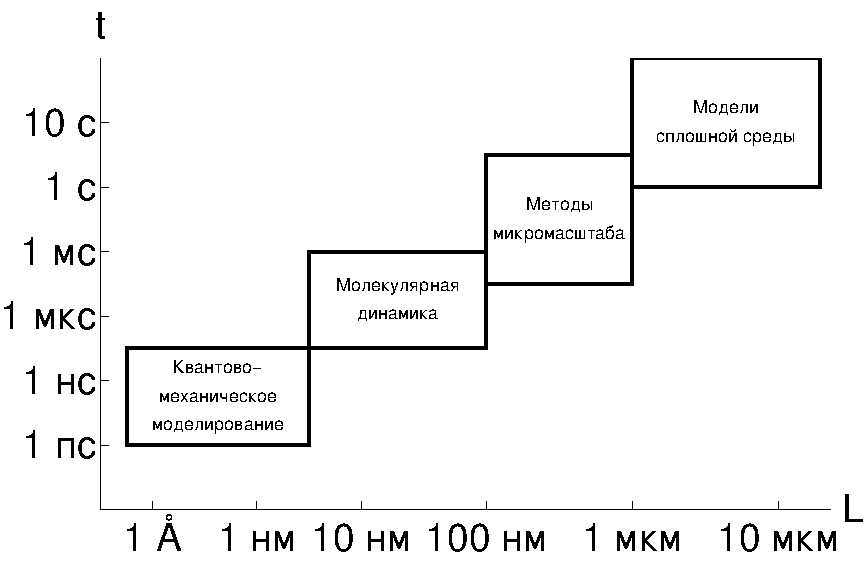
\includegraphics[width=0.85\textwidth]{pics/ModelsHierarchy.pdf}
    }
    \caption{Иерархия моделей.}\label{fig:ModelsHierarchy}
\end{figure}

Однако, несмотря на то, что модели молекулярной динамики и статистические модели находятся на более низких ступенях иерархии, чем модели сплошной среды, анализ объектов при помощи этих моделей без численных экспериментов крайне ограничен \cite{MDExperiment}. Поэтому с середины XX века набирают популярность модели обобщённой механики сплошной среды, которые распространяют применение моделей высшего уровня на области применения моделей низшего уровня. Одна из первых таких моделей была предложена в работе братьев Эжен и Франсуа Коссера \cite{Cosserat}, где помимо трансляционных степеней свободы также учитывались и вращательные компоненты движения, которые связаны с трансляционными рядом соотношений из-за чего тензор напряжений становится нессиметричным. Позже, спустя пол века, эта теория была связана с теорией дислокаций в работе V.~G{\"u}nther \cite{CosseratAndDislocation} и дополнена законом сохранения микроинерции в работе A.C.~Eringen \cite{Eringen2, Eringen3} в связи с чем теорию начали называть микрополярной теорией упругости. Также к работам связанным с исследованием микрополярной теории упругости можно отнести работы R.D.~Mindlin \cite{Mindlin1, Mindlin2, Mindlin3}, и работы D.B.~Bogy \cite{Bogy} и Y.C.~Hsu \cite{Hsu}, в которых авторы рассматривали применение этой теории к задачам с концентраторами возникающим в углах и отверстиях соответсвенно. В это же время теория приобрела своё развитие в работах советских учёных Э.Л.~Аэро и Е.В.~Кувшинского \cite{Aero1,Aero2}, а также была рассмотрена в работах Н.Ф.~Морозова \cite{Morozov} и Г.Н. Савина \cite{Savin}.

Дальнейшее развитие микрополярной теории упругости привело к появлению микроморфных моделей \cite{Eringen4, Micromorph1, Micromorph2}, в которые помимо вращательных компонент движения могут быть включены дополнительные переменные связанные с деформацией материала, при этом микрополярная теория упругости ялвяется лишь частным случаем микроморфных моделей. К сожалению, использование таких моделей сопряжено с трудностью определения материальных коэффициентов, которых в такого рода моделях становится достаточно много.

Список рассмотренных моментных моделей, а также авторов, которые занимались их развитием и исследованием далеко не исчерпывающий, однако, стоит также уделить внимание другому классу моделей обобщённой механики сплошной среды учитывающих дальнодействующие эффекты. Это градиентные и нелокальные модели, которые также получили своё развитие в 60-х годах XX века. Первые модели градиентной теории упругости были сформулированы в работах Toupin~R.A. \cite{Toupin} и Mindlin~R.D. \cite{Mindlin4, Mindlin5}, которые сейчас в литературе принято называть моделями Миндлина --- Тупина \cite{ToupinMindlin1, ToupinMindlin2, ToupinMindlin3}. Позже в работе G.~Ahmadi и K.~Firoozbakhsh \cite{GradientThermoelasticity} эти модели получили связь с температурными деформациями. Но как и микроморфные модели градиентные модели обладают тем же недостатком --- большое количество материальных констант, которые необходимо определить, поэтому в 90-х годах XX века в работах E.C.~Aifantis и его соавторов \cite{Aifantis1, Aifantis2} была рассмотренна упрощёная модель градиентной теории упругости, в которой напряжения зависят от деформации и её второго градиента, а также введён всего один дополнительный материальный параметр внутренней длины.

Нелокальные модели в отличие от градиентных оперируют интегральными выражениями типа свёртки. Впервые описание таких моделей было представлено в работе E.~Kr{\"o}ner \cite{Kroner}, где рассматривались упругие среды с дальнодействующими силами сцепления. Модели нелокальной упругости в термодинамическом контексте были рассмотрены в работах D.G.B.~Edelen, A.E.~Green и N.~Laws \cite{Edelen1, Edelen2}, позже к работе присоединился и A.C.~Eringen \cite{Eringen5, Eringen6}. Исследование условий обеспечивающих существование фундаментнальных решений было проведено в работе D. Rogula \cite{Rogula1982}. Вопросы, связанные с существованием и единственностью решения нелокальной начально-краевых задач упругости были рассмотрены в работах S.B.~Altan \cite{Altan1, Altan2}, а также для задач нелокальной термоупругости \cite{Altan3, Altan4}. В дальнейшем A.C.~Eringen представит работу, в которой описан единый подход к построению нелокальных теорий для упругих тел в работе \cite{Eringen1}, в связи с чем в литературе нелокальные модели часто называют моделями Эрингена \cite{BondaryLayer, Tuna, Rahmani}.

Связь градиентной модели Айфантиса и нелокальной \cite{Aifantis3, Gao}.

Текущая работа посвящена исследованию нелокальных моделей, а точнее даже их модификации с добавлением регуляризационного слагаемого относящегося к классической или локальной теории. Такой подход был предложен в работе Polizzoto \cite{Polizzotto1}.

\cite{SaintVenant}.

Поиск решений интегро-дифференциальных уравнений представляет из себя достаточно сложную задачу. В этом случае необходимо прибегать к использованию различных численных методов, специально адаптированных под данный класс уравнений. В этом направлении есть уже достаточно большое количество работ, предлагающие использовать различные методы решения. Наиболее общим и популярным является метод конечных элементов (FEM), который применительно к данному классу уравнений иногда ещё называют методом нелокальных конечных элементов (NL-FEM) \cite{Polizzotto2, Pisano1}. Однако его использование сопряжёно с большой вычислительной сложностью, поэтому некоторые ииследователи прибегают к возможностям интегральных преобразований откуда был получен метод на основе быстрого преобразования Гаусса (FEMFGT) \cite{FastGaussTransform}. К сожалению, использование этого метода сопряжено с рядом трудностей, так как для его применения необходима достаточно подробная сетка, чтобы избежать возможных осциляций решения, также сложность вызывает контроль точности получаемых решений. Помимо сеточных методов большой популярностью пользуются и бессеточные подходы на основе радиальных базисных функций \cite{RadialBasis}, безэлементный метод Галёркина (EFG) и метод конечных точек (FPM) \cite{MeshFree}. Также были предложены подходы с использованием пограничного слоя \cite{BondaryLayer} и на основе полиномов Чебышева \cite{ChebPolynom}.

В рамках этой работы было принято решение остановиться на методе конечных элементов, так как этот метод достаточно хорошо изучен и его относительно легко реализовать и модифицировать под рассматриваемый класс уравнений. Также этим методом легко решать задачи на областях со сложной геометрической формой, а большое количество редакторов и генераторов сеток упрощает процесс моделирования. Реализация данного метода включена в программный комплекс NonLocFEM, структуру которого мы рассмотрим в третьей главе диссертации.

%\ifsynopsis
%Этот абзац появляется только в~автореферате.
%\else
%Этот абзац появляется только в~диссертации.
%\fi

% {\progress}
% Этот раздел должен быть отдельным структурным элементом по
% ГОСТ, но он, как правило, включается в описание актуальности
% темы. Нужен он отдельным структурынм элемементом или нет ---
% смотрите другие диссертации вашего совета, скорее всего не нужен.

{\aim}
исследования является изучение особенностей рассматриваемых моделей термоупругости, а также сравнение решений полученных при их использовании с решениями полученными при использовании классических моделей механики сплошной среды.

Для достижения поставленной цели потребовалось решить {\tasks}:
\begin{enumerate}[beginpenalty=10000] % https://tex.stackexchange.com/a/476052/104425
  \item Разработка определяющих соотношений модели термоупругости нелокальной среды в интегро-дифференциальной форме..
  \item Разработка алгоритмов численного решения с их последующей оптизацией для более эффективного использования на многопроцессорных вычислительных машинах.
  \item Реализация полученных алгоритмов в виде программного комплекса.
  \item Исследование поведения модели на примере решения определённого ряда задач с известными решениями в классической постановке, сравнение получившихся решений и определение закономерностей.
\end{enumerate}


{\novelty}
\begin{enumerate}[beginpenalty=10000] % https://tex.stackexchange.com/a/476052/104425
  \item Разработаны эффективные методы решения на основе метода конечных элементов с обобщением на интегро-дифференциальные уравнения, которые обладают хорошей масштабируемостью и предназначены для вычислений на многопроцессорных вычислительных машинах с общей и распределённой памятью.
  \item Разработан программный комплекс NonLocFEM, в котором реализованы все представленные в работе алгоритмы и методы для моделирования поведения структруно-чувствительных материалов.
  \item Проведено качественное сравнение между результатами полученными с использованием классической и нелокальной теориями, которые свидетельствуют о снижении роли концентраторов в распределениях полей напряжений и плотности теплового потока.
  \item Исследованы границы спектров собственных чисел матриц и установлены связи между спектрами матриц ассемблированных в классической и нелокальной постановках.
\end{enumerate}

{\influence}
моделей рассмотренных в диссертации состоит в возможности описания поведения термомеханических состояний структурно-чувствительных материалов, параметры модели очевидным образом влияют на решения, что позволяет тонко настраивать модель при исследованиях. Разработанный программный комплекс дополняет рассматриваемую модель, позволяет проводить расчёты на произвольных областях со всеми рассматриваемыми в моделе параметрами, а благодаря открытому исходному код и модульной структуре существует возможность без труда вносить в него изменения и добавлять новые типы расчётов при модификации математической модели.

{\methods}
В диссертации используются как классические принципы механики деформируемого твёрдого тела, так и новые относящиеся к нелокальной теории термоупругости, а также численные методы в основе которых лежит метод конечных элементов.

{\defpositions}
\begin{enumerate}[beginpenalty=10000] % https://tex.stackexchange.com/a/476052/104425
 	\item Модель нелокальной термоупругости позволяющая описать процессы теплопроводности и напряжённо-деформированного состояния в структурно-чувствительных материалах.
	\item Численный алгоритм решения на основе метода конечных элементов, адапатированный под многопроцессорные вычислительные системы.
	\item Программный комплекс NonLocFEM, в рамках которого реализованы все рассматриваемые в работе методы решений.
\end{enumerate}

{\reliability} гарантирует строгость используемого математического аппарата, сравнение расчётов с известными теоретическими результатами и аналитическими решениям, а также результатами, полученными ранее другими авторами.


{\probation}
проводилась в обсуждениях на следующих конференциях:
\begin{enumerate}
	\item Международная научно-техническая конференция <<Актуальные проблемы прикладной математики, информатикии и механики>> (Воронеж, 2019, 2021);
	\item Международная конференция <<International Conference of Numerical Analysis and Applied Mathematics>> (Родос, Греция, 2021);
	\item Международная научная конференция <<Фундаментальные и Прикладные Задачи Механики>> (Москва, 2021);
	\item Всероссийская конференция по численным методам решения задач теории упругости и пластичности (Красноярск, 2023);
	\item Математическое моделирование, численные методы и инженерное программное обеспечение (Москва, 2023).
\end{enumerate}

{\contribution}
Все исследования, представленные в диссертационной работе, а также разработка программного комплекса выполнены лично соискателем в процессе научной деятельности. Из совместных публикаций в диссертацию включен лишь тот материал, который принадлежит соискателю, заимствованный материал обозначен в работе ссылками.

\ifnumequal{\value{bibliosel}}{0}
{%%% Встроенная реализация с загрузкой файла через движок bibtex8. (При желании, внутри можно использовать обычные ссылки, наподобие `\cite{vakbib1,vakbib2}`).
    {\publications} Основные результаты по теме диссертации изложены
    в~XX~печатных изданиях,
    X из которых изданы в журналах, рекомендованных ВАК,
    X "--- в тезисах докладов.
}%
{%%% Реализация пакетом biblatex через движок biber
    \begin{refsection}[bl-author, bl-registered]
        % Это refsection=1.
        % Процитированные здесь работы:
        %  * подсчитываются, для автоматического составления фразы "Основные результаты ..."
        %  * попадают в авторскую библиографию, при usefootcite==0 и стиле `\insertbiblioauthor` или `\insertbiblioauthorgrouped`
        %  * нумеруются там в зависимости от порядка команд `\printbibliography` в этом разделе.
        %  * при использовании `\insertbiblioauthorgrouped`, порядок команд `\printbibliography` в нём должен быть тем же (см. biblio/biblatex.tex)
        %
        % Невидимый библиографический список для подсчёта количества публикаций:
        \printbibliography[heading=nobibheading, section=1, env=countauthorvak,          keyword=biblioauthorvak]%
        \printbibliography[heading=nobibheading, section=1, env=countauthorwos,          keyword=biblioauthorwos]%
        \printbibliography[heading=nobibheading, section=1, env=countauthorscopus,       keyword=biblioauthorscopus]%
        \printbibliography[heading=nobibheading, section=1, env=countauthorconf,         keyword=biblioauthorconf]%
        \printbibliography[heading=nobibheading, section=1, env=countauthorother,        keyword=biblioauthorother]%
        \printbibliography[heading=nobibheading, section=1, env=countregistered,         keyword=biblioregistered]%
        \printbibliography[heading=nobibheading, section=1, env=countauthorpatent,       keyword=biblioauthorpatent]%
        \printbibliography[heading=nobibheading, section=1, env=countauthorprogram,      keyword=biblioauthorprogram]%
        \printbibliography[heading=nobibheading, section=1, env=countauthor,             keyword=biblioauthor]%
        \printbibliography[heading=nobibheading, section=1, env=countauthorvakscopuswos, filter=vakscopuswos]%
        \printbibliography[heading=nobibheading, section=1, env=countauthorscopuswos,    filter=scopuswos]%
        %
        \nocite{*}%
        %
        {\publications} Основные результаты по теме диссертации изложены в~\arabic{citeauthor}~печатных изданиях,
        \arabic{citeauthorvak} из которых изданы в журналах, рекомендованных ВАК\sloppy%
        \ifnum \value{citeauthorscopuswos}>0%
            , \arabic{citeauthorscopuswos} "--- в~периодических научных журналах, индексируемых Web of~Science и Scopus\sloppy%
        \fi%
        \ifnum \value{citeauthorconf}>0%
            , \arabic{citeauthorconf} "--- в~тезисах докладов.
        \else%
            .
        \fi%
        \ifnum \value{citeregistered}=1%
            \ifnum \value{citeauthorpatent}=1%
                Зарегистрирован \arabic{citeauthorpatent} патент.
            \fi%
            \ifnum \value{citeauthorprogram}=1%
                Зарегистрирована \arabic{citeauthorprogram} программа для ЭВМ.
            \fi%
        \fi%
        \ifnum \value{citeregistered}>1%
            Зарегистрированы\ %
            \ifnum \value{citeauthorpatent}>0%
            \formbytotal{citeauthorpatent}{патент}{}{а}{}\sloppy%
            \ifnum \value{citeauthorprogram}=0 . \else \ и~\fi%
            \fi%
            \ifnum \value{citeauthorprogram}>0%
            \formbytotal{citeauthorprogram}{программ}{а}{ы}{} для ЭВМ.
            \fi%
        \fi%
        % К публикациям, в которых излагаются основные научные результаты диссертации на соискание учёной
        % степени, в рецензируемых изданиях приравниваются патенты на изобретения, патенты (свидетельства) на
        % полезную модель, патенты на промышленный образец, патенты на селекционные достижения, свидетельства
        % на программу для электронных вычислительных машин, базу данных, топологию интегральных микросхем,
        % зарегистрированные в установленном порядке.(в ред. Постановления Правительства РФ от 21.04.2016 N 335)
    \end{refsection}%
    \begin{refsection}[bl-author, bl-registered]
        % Это refsection=2.
        % Процитированные здесь работы:
        %  * попадают в авторскую библиографию, при usefootcite==0 и стиле `\insertbiblioauthorimportant`.
        %  * ни на что не влияют в противном случае
        \nocite{vakbib2}%vak
        \nocite{patbib1}%patent
        \nocite{progbib1}%program
        \nocite{bib1}%other
        \nocite{confbib1}%conf
    \end{refsection}%
        %
        % Всё, что вне этих двух refsection, это refsection=0,
        %  * для диссертации - это нормальные ссылки, попадающие в обычную библиографию
        %  * для автореферата:
        %     * при usefootcite==0, ссылка корректно сработает только для источника из `external.bib`. Для своих работ --- напечатает "[0]" (и даже Warning не вылезет).
        %     * при usefootcite==1, ссылка сработает нормально. В авторской библиографии будут только процитированные в refsection=0 работы.
}

%При использовании пакета \verb!biblatex! будут подсчитаны все работы, добавленные
%в файл \verb!biblio/author.bib!. Для правильного подсчёта работ в~различных
%системах цитирования требуется использовать поля:
%\begin{itemize}
%        \item \texttt{authorvak} если публикация индексирована ВАК,
%        \item \texttt{authorscopus} если публикация индексирована Scopus,
%        \item \texttt{authorwos} если публикация индексирована Web of Science,
%        \item \texttt{authorconf} для докладов конференций,
%        \item \texttt{authorpatent} для патентов,
%        \item \texttt{authorprogram} для зарегистрированных программ для ЭВМ,
%        \item \texttt{authorother} для других публикаций.
%\end{itemize}
%Для подсчёта используются счётчики:
%\begin{itemize}
%        \item \texttt{citeauthorvak} для работ, индексируемых ВАК,
%        \item \texttt{citeauthorscopus} для работ, индексируемых Scopus,
%        \item \texttt{citeauthorwos} для работ, индексируемых Web of Science,
%        \item \texttt{citeauthorvakscopuswos} для работ, индексируемых одной из трёх баз,
%        \item \texttt{citeauthorscopuswos} для работ, индексируемых Scopus или Web of~Science,
%        \item \texttt{citeauthorconf} для докладов на конференциях,
%        \item \texttt{citeauthorother} для остальных работ,
%        \item \texttt{citeauthorpatent} для патентов,
%        \item \texttt{citeauthorprogram} для зарегистрированных программ для ЭВМ,
%        \item \texttt{citeauthor} для суммарного количества работ.
%\end{itemize}
% Счётчик \texttt{citeexternal} используется для подсчёта процитированных публикаций;
% \texttt{citeregistered} "--- для подсчёта суммарного количества патентов и программ для ЭВМ.

%Для добавления в список публикаций автора работ, которые не были процитированы в
%автореферате, требуется их~перечислить с использованием команды \verb!\nocite! в
%\verb!Synopsis/content.tex!.
 % Характеристика работы по структуре во введении и в автореферате не отличается (ГОСТ Р 7.0.11, пункты 5.3.1 и 9.2.1), потому её загружаем из одного и того же внешнего файла, предварительно задав форму выделения некоторым параметрам

\textbf{Объем и структура работы.} Диссертация состоит из~введения,
\formbytotal{totalchapter}{глав}{ы}{}{},
заключения и 1 приложения.
%\formbytotal{totalappendix}{приложен}{ия}{ий}{}.
%% на случай ошибок оставляю исходный кусок на месте, закомментированным
%Полный объём диссертации составляет  \ref*{TotPages}~страницу
%с~\totalfigures{}~рисунками и~\totaltables{}~таблицами. Список литературы
%содержит \total{citenum}~наименований.
%
Полный объём диссертации составляет
\formbytotal{TotPages}{страниц}{у}{ы}{}, включая
\formbytotal{totalcount@figure}{рисун}{ок}{ка}{ков} и
\formbytotal{totalcount@table}{таблиц}{у}{ы}{}.
Список литературы содержит
\formbytotal{citenum}{наименован}{ие}{ия}{ий}.
    % Введение
\ifnumequal{\value{contnumfig}}{1}{\counterwithout{figure}{chapter}
}{\counterwithin{figure}{chapter}}
\ifnumequal{\value{contnumtab}}{1}{\counterwithout{table}{chapter}
}{\counterwithin{table}{chapter}}
\chapter{Основные соотношения}\label{ch:BasicRelations} 

\section{Определение нелокального оператора}\label{sec:BasicRelations/NonlocalOperator}

Определим линейный интегральный оператор $\mathcal{N}$, который представим в виде взвешенной суммы, где первое слагаемое --- это подставляемое в оператор выражение с весовым множителем $p_1$, а второе --- это же выражение, но взвешенное по области $S'(\boldsymbol{x})$ с некоторой весовой функцией $\varphi$ и весовым параметром $p_2$,
\begin{gather}
	\label{eq:IntegroDiffOperator}
	\mathcal{N} [f(\boldsymbol{x})] = 
	p_1 f(\boldsymbol{x}) + 
	p_2 \int\limits_{S'(\boldsymbol{x}') \cap S} 
		\varphi(\boldsymbol{x}, \boldsymbol{x}') f(\boldsymbol{x}')
	dS'(\boldsymbol{x}'),
	\quad
	\boldsymbol{x}' \in S'(\boldsymbol{x}).
\end{gather}
Здесь $f(\boldsymbol{x})$ --- некоторое выражение, описывающее сохраняющуюся физическую субстанцию;
$p_1 > 0$ и $p_2 \geqslant 0$ --- весовые параметры модели такие, что $p_1 + p_2 = 1$;
$\varphi$~---~функция нелокального влияния, некоторая нормированная положительная монотонно убывающая функция в области $S'(\boldsymbol{x})$; 
$\boldsymbol{x}'$ --- точка в области $S'(\boldsymbol{x})$, в которой вычисляется влияние на величины находящиеся в точке $\boldsymbol{x}$;
$S'(\boldsymbol{x})$ --- область нелокального влияния с центром в точке $\boldsymbol{x} \in S$;
$S$ --- область занимаемая рассматриваемым телом.

Отметим, что для каждого отдельно взятого физического процесса $\mathcal{F}$ можно определить свой собственный оператор $\mathcal{N}_\mathcal{F}$ со своим набором весовых констант $p_1$ и $p_2$, функцией нелокального влияния $\varphi$ и областью нелокального влияния $S'(\boldsymbol{x})$. Однако для упрощения дальнейших выкладок, без потери общности, ограничимся гипотезой, что для тепловых и механических задач параметры нелокальности одинаковые.

\section{Уравнение стационарной теплопроводности}\label{sec:BasicRelations/HeatEquation}

В произвольной замкнутой области $S \subset \mathbb{R}^2$ с кусочно-гладкой границей $\partial S$ уравнение стационарной теплопроводности имеет вид \cite{MSS}
\begin{gather}
	\label{eq:StationaryHeatEquation}
	\nabla \cdot \boldsymbol{q} = q_V,
\end{gather}
где $q_V$ --- объёмная плотность мощности внутренних источников и стоков теплоты;
$\boldsymbol{q}$ --- вектор плотности теплового потока, который можно определить как обобщение гипотезы Био --- Фурье \cite{ThermoViscoElasticity1, ThermoViscoElasticity2, ThermoViscoElasticity3}, подставив её в \mbox{оператор~(\ref{eq:IntegroDiffOperator})}
\begin{gather}
	\label{eq:BiotFourier}
	\boldsymbol{q}(\boldsymbol{x}) = 
	\mathcal{N} \left( -\widehat{\boldsymbol{\lambda}} \cdot \nabla T \right),
\end{gather}
где $\widehat{\boldsymbol{\lambda}} = \lambda_{ij} \boldsymbol{e}_i \otimes \boldsymbol{e}_j$ --- тензор коэффициентов теплопроводности;
$T$ --- поле температуры.

Граничные условия первого, второго и третьего родов для уравнения (\ref{eq:StationaryHeatEquation}) имеют вид
\begin{gather}
	\label{eq:ThermalBoundaries}
	T|_{\Gamma_1} = T_{\Gamma} (\boldsymbol{x}),
	\quad
	\boldsymbol{n} \cdot \boldsymbol{q}|_{\Gamma_2} = f(\boldsymbol{x}),
	\quad
	\boldsymbol{n} \cdot \boldsymbol{q}|_{\Gamma_3} = \alpha (T_a(\boldsymbol{x}) - T(\boldsymbol{x}))),
\end{gather}
где $\Gamma_1 \cup \Gamma_2 \cup \Gamma_3 = \partial S$, $\Gamma_1 \cap \Gamma_2 = \Gamma_1 \cap \Gamma_3 = \Gamma_2 \cap \Gamma_3 = \varnothing$;
$T_{\Gamma} (\boldsymbol{x})$ и $f(\boldsymbol{x})$ --- некоторые функции, задающие температуру и плотность теплового потока на границах $\Gamma_1$ и $\Gamma_2$ соответственно;
$\alpha$ --- коэффициент конвективного теплообмена со средой;
$T_a (\boldsymbol{x})$ --- температура среды вблизи границы $\Gamma_3$.
Для простоты дальнейшего изложения будем предполагать, что функции $T_{\Gamma}(\boldsymbol{x})$, $f(\boldsymbol{x})$ и $T_a(\boldsymbol{x})$ равны нулю во множествах, где они не определены.

\section{Уравнение равновесия}\label{sec:BasicRelations/EquilibriumEquation}

В произвольной замкнутой области $S \subset \mathbb{R}^2$ с кусочно-гладкой границей $\partial S$ можем определить уравнение равновесия сплошной среды \cite{MSS}
\begin{gather}
	\label{eq:EquilibriumEquation}
    \nabla \cdot \widehat{\boldsymbol{\sigma}} = \boldsymbol{b},
\end{gather}
где $\boldsymbol{b} = b_i \boldsymbol{e}_i$ --- вектор плотности объёмных сил;
$\widehat{\boldsymbol{\sigma}} = \sigma_{ij} \boldsymbol{e}_i \otimes \boldsymbol{e}_j$ --- тензор напряжений, который для случая несвязанной термоупругой задачи определим как обобщение закона Дюамеля --- Неймана с использованием оператора (\ref{eq:IntegroDiffOperator}) \cite{ThermoViscoElasticity1, ThermoViscoElasticity2, ThermoViscoElasticity3}
\begin{gather}
	\label{eq:DuamelNeumann}
	\widehat{\boldsymbol{\sigma}}(\boldsymbol{x}) =
	\mathcal{N} \left(
		\widehat{\text{\textbf{C}}} \cdot \cdot 
		\left( \widehat{\boldsymbol{\varepsilon}} - \widehat{\boldsymbol{\alpha}}^T \Delta T \right)
	\right),
\end{gather}
где \mbox{$\widehat{\varepsilon} = \varepsilon_{ij} \boldsymbol{e}_i \otimes \boldsymbol{e}_j$}~---~тензор деформации;
$\widehat{\text{\textbf{C}}} = C_{ijkl} \boldsymbol{e}_i \otimes \boldsymbol{e}_j \otimes \boldsymbol{e}_k \otimes \boldsymbol{e}_l$ --- тензор коэффициентов упругости;
$\widehat{\boldsymbol{\alpha}}^T = \alpha_{ij}^T \boldsymbol{e}_i \otimes \boldsymbol{e}_j$ --- тензор температурных коэффициентов линейного расширения;
$\Delta T = T - T_0$ --- разница между текущим распределением температуры $T$ и распределением $T_0$ при котором отсутствуют температурные деформации.

Далее примем, что тело является линейно-упругим и изотропным. В случае плоского напряжённого состоянии, компоненты тензора упругости $\widehat{\text{\textbf{C}}}$ будут определены следующим образом \cite{MSS}
\begin{gather*}
	C_{ijkl} =
	\dfrac{\nu E}{1 - \nu^2} \delta_{ij} \delta_{kl} +
	\dfrac{E}{2(1 + \nu)} (\delta_{ik} \delta_{jl} + \delta_{il} \delta_{jk}),
\end{gather*}
где $E$ --- модуль Юнга;
$\nu$ --- коэффициент Пуассона;
$\delta_{ij}$ --- дельта Кронекера.
Если же рассмотрен случай плоского деформированного состояния, то компоненты тензора упругости имеют аналогичную форму записи
\begin{gather*}
	C_{ijkl} =
	\dfrac{\widetilde{\nu} \widetilde{E}}{1 - \widetilde{\nu}^2} \delta_{ij} \delta_{kl} +
	\dfrac{\widetilde{E}}{2(1 + \widetilde{\nu})} (\delta_{ik} \delta_{jl} + \delta_{il} \delta_{jk}),
\end{gather*}
однако, здесь $\widetilde{E} = E / (1 - \nu^2)$ и $\widetilde{\nu} = \nu / (1 - \nu)$. Для изотропной среды будем считать, что тело расширяется равнонаправлено, поэтому тензор температурных коэффициентов линейного расширения будет диагональным и иметь всего один коэффициент $\alpha^T$, то есть \cite{MSS}
\begin{gather*}
	\widehat{\boldsymbol{\alpha}}^T = \alpha^T \widehat{\text{\textbf{I}}}_2.
\end{gather*}

Примем гипотезу, что деформации достаточно малы, поэтому для определения компонент тензора деформации $\widehat{\boldsymbol{\varepsilon}}$ воспользуемся соотношениями \mbox{Коши \cite{MSS}}
\begin{gather*}
	\widehat{\boldsymbol{\varepsilon}} = 
	\dfrac{\boldsymbol{u} + (\nabla \boldsymbol{u})^T}{2} = 
	\dfrac{u_{i, j} + u_{j, i}}{2} \boldsymbol{e}_i \otimes \boldsymbol{e}_j,
\end{gather*}
где $\boldsymbol{u}$ --- вектор перемещения.

Будем рассматривать граничные условия первого и второго родов, также именуемые кинематическими и силовыми соответственно,
\begin{gather}
	\label{eq:StressBoundaries}
	\boldsymbol{u}|_{\Gamma_4} = \boldsymbol{d} (\boldsymbol{x}),
	\quad
	\boldsymbol{n} \cdot \widehat{\boldsymbol{\sigma}}|_{\Gamma_5} = \boldsymbol{p} (\boldsymbol{x}),
\end{gather}
где $\boldsymbol{d} (\boldsymbol{x}) = d_i (\boldsymbol{x}) \boldsymbol{e}_i$ --- вектор перемещений на границе $\Gamma_4$;
$\boldsymbol{p} (\boldsymbol{x}) = p_i (\boldsymbol{x}) \boldsymbol{e}_i$ --- вектор плотности поверхностностного нагружения на границе $\Gamma_5$. Помимо этого будем рассматривать комбинированные граничные условия, когда по одной компоненте задано перемещение, а по другой поверхностное нагружение. Как и в случае с граничными условиями уравнения теплопроводности, для простоты будем считать, что функции задающие граничные условия уравнения равновесия (\ref{eq:DuamelNeumann}) будут равны нулю на границах, на которых они не определены.

\section{Определение области и функции нелокальности}\label{sec:BasicRelations/InfluenceFunction}

В определении оператора (\ref{eq:IntegroDiffOperator}) нет ограничения на выбор области нелокального влияния $S'(\boldsymbol{x})$. Она  может быть как неограниченной и включать в себя всю рассчётную область, так и замкнутой, покрывая лишь часть рассматриваемого тела. В любом случае, выбор области $S'(\boldsymbol{x})$ подразумевает так же и выбор функции нелокального влияния $\varphi$. С практической точки зрения, следует выбирать такую функцию $\varphi$, чтобы интеграл от неё по области $S'(\boldsymbol{x})$ был в рамках заданной точности близким к единице \cite{Eringen3}. Вместе с этим область $S'(\boldsymbol{x})$ должна быть достаточной для аппроксимации наблюдаемых явлений, но в то же время, она не должна покрывать всю область занимаемую телом, так как на практике при аппроксимации уравнений это позволит использовать разреженные матрицы для хранения коэффициентов СЛАУ \cite{Pisanetzkiy} и значительно облегчит численные расчёты, повысив общую эффективность использования вычислительных ресурсов. 

Однако выбор области нелокального влияния $S'(\boldsymbol{x})$ является нетривиальной задачей, где в первую очередь стоит опираться на структуру рассматриваемого материала \cite{Eringen3}. Поэтому рассмотрим наиболее общий (пусть и не исчерпывающий) случай и представим $S'(\boldsymbol{x})$ в виде фигуры ограниченной суперэллипсом \cite{Superellipse}, изображённой на Рис.~\ref{fig:SuperEllipse} при различных параметрах $n > 0$. У такого семейства фигур есть также параметры, отвечающие за длины главных полуосей $r_1 > 0$ и $r_2 > 0$. На основе этих параметров можем определить метрическую функцию
\begin{gather}
	\label{eq:metricFunction}
	\rho_n(\boldsymbol{x}, \boldsymbol{x}') = 
	\left(
		\left| \dfrac{x_1 - x_1'}{r_1} \right|^n +
		\left| \dfrac{x_2 - x_2'}{r_2} \right|^n
	\right)^{\dfrac{1}{n}},
\end{gather}
использовав которую приступим к построению всевозможных функций нелокального влияния $\varphi$, соблюдая правило, что функция $\varphi$ должна монотонно убывать по мере роста функции $\rho_n$.

\begin{figure}[ht]
    \centerfloat{
        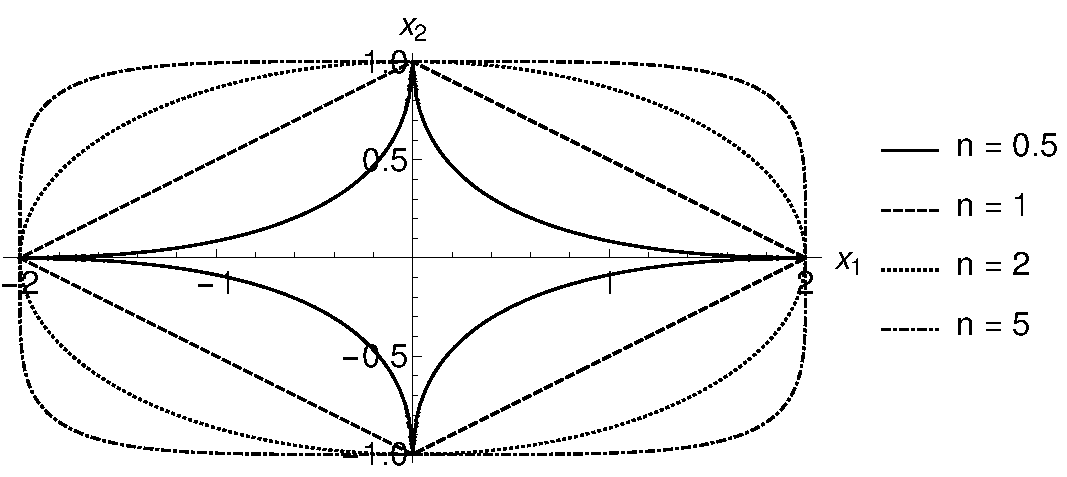
\includegraphics[width=0.85\textwidth]{pics/SuperEllipse.pdf}
    }
    \caption{Cуперэллипсы при различных параметрах $n$}\label{fig:SuperEllipse}
\end{figure}

Воспользовавшись метрической функцией $\rho_n$ (\ref{eq:metricFunction}), построим семейство полиномиальных функций нелокального влияния, определённых в ограниченной области \cite{PolyInfluence},
\begin{gather}
	\label{eq:polynomialInfluence}
	\varphi_{p,q}^{P}(\boldsymbol{x}, \boldsymbol{x}') =
	\begin{cases}
		A(1 - \rho_n(\boldsymbol{x}, \boldsymbol{x}')^p)^q, \quad &\rho_n(\boldsymbol{x}, \boldsymbol{x}') \leqslant 1, \\
		0, &\rho_n(\boldsymbol{x}, \boldsymbol{x}') > 1,
	\end{cases}
\end{gather}
где $p > 0$ и $q > 0$ --- параметры управляющие плотностью распределения функции. На Рис.~\ref{fig:PolynomialInfluencePortrait} продемонстрировано, что увеличение параметра $p$ делает распределение функции более равномерным и в пределе распределение стремится к константе обратно пропорциональной площади заключённой в область $S'(\boldsymbol{x})$, а увеличение параметра $q$ концентрирует распределение в центре области и в пределе распределение стремится к дельта-функции Дирака; множитель $A$ является нормировочным и в общем случае он равен следующему значению
\begin{gather*}
	A = \dfrac{np}
	{
		4 r_1 r_2 
		\operatorname{B}\left( \dfrac{1}{n}, \dfrac{1}{n} \right) 
		\operatorname{B}\left( \dfrac{2}{p}, q+1 \right)
	}.
\end{gather*}
Отдельно отметим, что при стремлении параметра $n$ к бесконечности, нормировочный множитель принимает значение
\begin{gather*}
	A = \dfrac{p}{8 r_2 r_2 \operatorname{B}\left( \dfrac{2}{p}, q+1 \right)},
\end{gather*}
а метрическая функция $\rho_n$ (\ref{eq:metricFunction}) вырождается в следующую
\begin{gather}
	\label{eq:metricFunctionInfinity}
	\rho_{\infty} (\boldsymbol{x}, \boldsymbol{x}') = 
	\max \left( 
		\left| \dfrac{x_1 - x_1'}{r_1} \right|,
		\left| \dfrac{x_2 - x_2'}{r_2} \right|
	\right).
\end{gather}
Далее при использовании данного семейства функций, в случае когда длины полуосей $r_1$ и $r_2$ равны, будем обозначать их одним символом $r$ и называть его радиусом нелокальности.

\begin{figure}[ht]
    \begin{minipage}[b][][b]{0.49\linewidth}\centering
        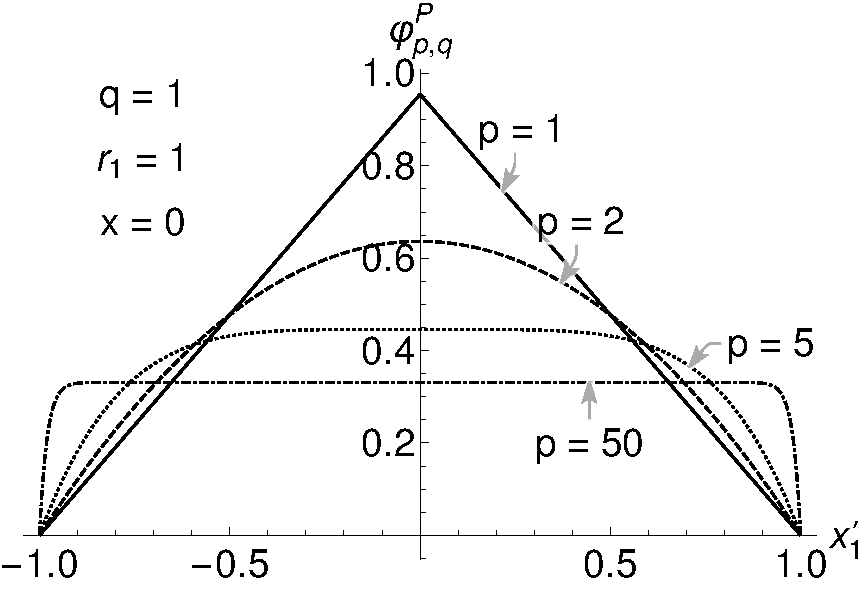
\includegraphics[width=\linewidth]{pics/PolynomialInfluenceP.pdf} \\ а)
    \end{minipage}
    \hfill
    \begin{minipage}[b][][b]{0.49\linewidth}\centering
        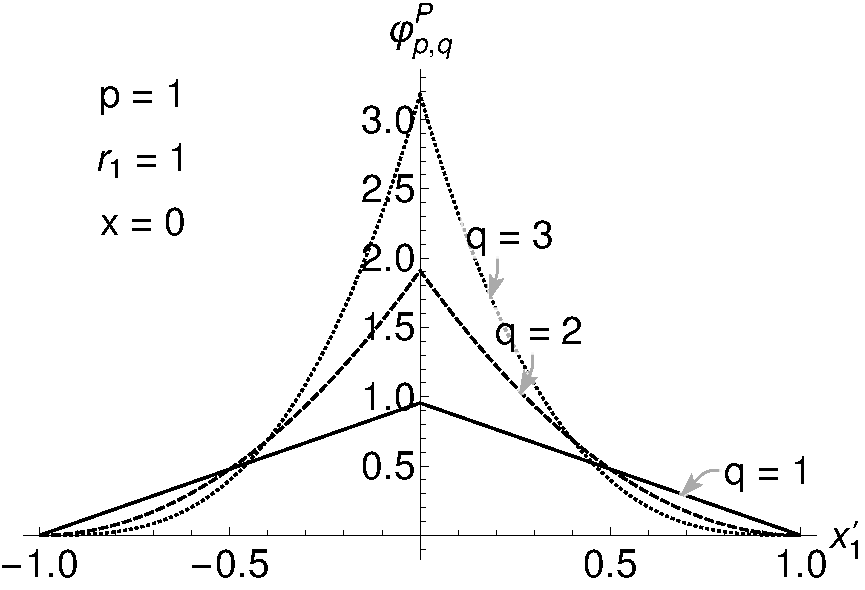
\includegraphics[width=\linewidth]{pics/PolynomialInfluenceQ.pdf} \\ б)
    \end{minipage}
    \caption{Портреты полиномиальных функций влияния в сечении вдоль оси $x'_1$ при вариации (а) параметра $p$ и (б) параметра $q$}
    \label{fig:PolynomialInfluencePortrait}
\end{figure}

Аналогично можем определить семейство экспоненциальных функций, для которых область влияния бесконечная
\begin{gather}
	\label{eq:exponentiallInfluence}
	\varphi_{p,q}^{E} (\boldsymbol{x}, \boldsymbol{x}') =
	A \exp \left(-q\rho_n(\boldsymbol{x}, \boldsymbol{x}')^p \right).
\end{gather}
Здесь параметры $p > 0$ и $q > 0$ имеют тот же смысл, что и у полиномиального семейства функций (\ref{eq:polynomialInfluence}). Это продемонстрировано на Рис.~\ref{fig:ExponentialInfluencePortrait}, однако, вместе с вариацией этих параметров следует также подбирать и параметры $r_1$ и $r_2$ подходящие под рассматриваемую расчётную область $S'(\boldsymbol{x})$, чтобы соблюсти нормировку. Нормировочный множитель $A$ в общем случае равен
\begin{gather}
	\label{eq:normExp}
	A = 
	\dfrac
	{
		4^{\frac{1}{n}} n p q^{\frac{2}{p}}
	}
	{
		8 r_1 r_2 \operatorname{B} \left( \dfrac{1}{2}, \dfrac{1}{n} \right) \operatorname{\Gamma} \left( \dfrac{2}{p} \right)
	}
\end{gather}
и при стремлении $n$ к бесконечности он принимает значение
\begin{gather*}
	A = \dfrac{p q^{\frac{2}{p}}}{8 r_1 r_2 \Gamma \left( \dfrac{2}{p} \right)}.
\end{gather*}
Обратим внимание, что при $q = 0.5$, $p = 2$ и $n = 2$ получаем функцию нормального распределения Гаусса, для которой параметры $r_1$ и $r_2$ можно определить по правилу <<3 сигма>> \cite{TeorVer}. Здесь, как и в случае с полиномиальным семейством функций, в случае равенства $r_1$ и $r_2$, будем обозначать их одним символом $r$, но называть его будем дисперсионным параметром нелокальности.

\begin{figure}[ht]
    \begin{minipage}[b][][b]{0.49\linewidth}\centering
        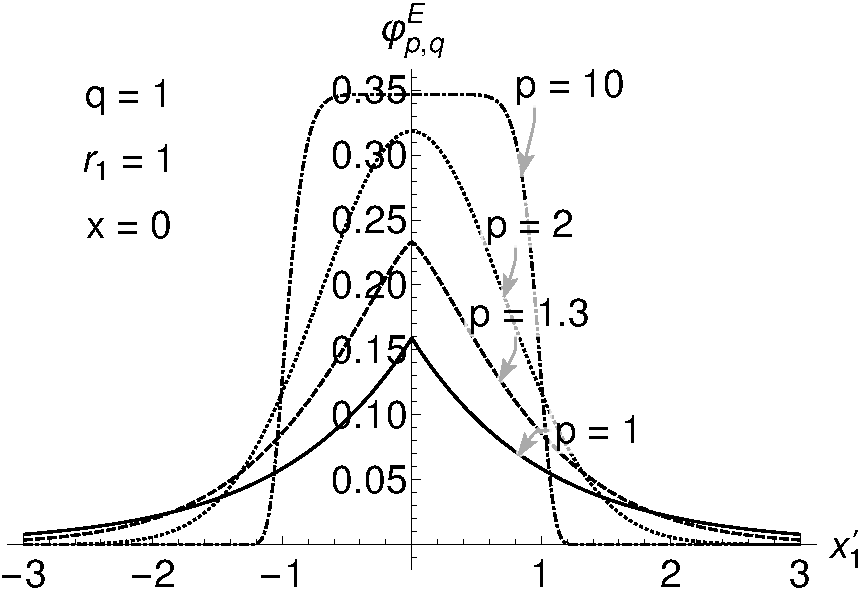
\includegraphics[width=\linewidth]{pics/ExponentialInfluenceP.pdf} \\ а)
    \end{minipage}
    \hfill
    \begin{minipage}[b][][b]{0.49\linewidth}\centering
        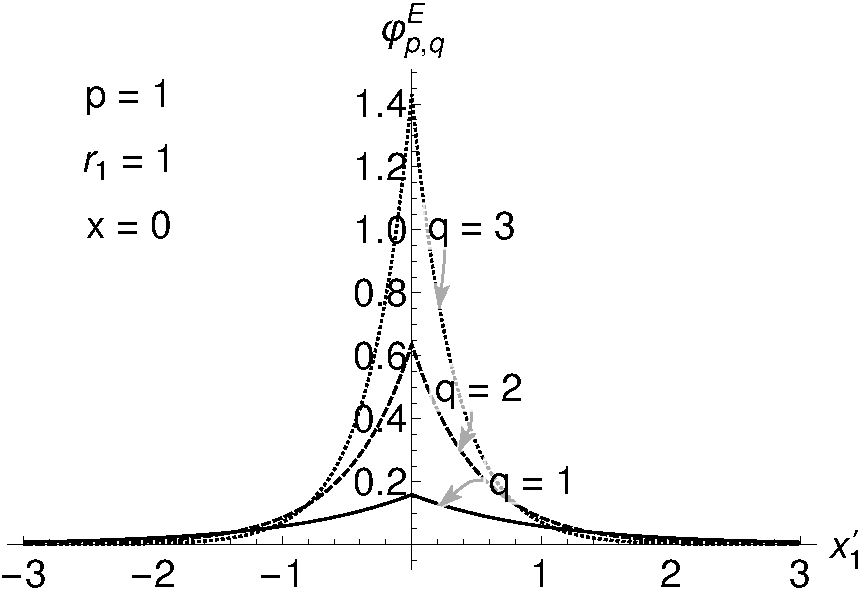
\includegraphics[width=\linewidth]{pics/ExponentialInfluenceQ.pdf} \\ б)
    \end{minipage}
    \caption{Портреты экспоненциальных функций влияния в сечении вдоль оси $x'_1$ при вариации (а) параметра $p$ и (б) параметра $q$}
    \label{fig:ExponentialInfluencePortrait}
\end{figure}

Для экспоненциального семейства функций возникает потребность в определении параметров $r_1$ и $r_2$. Для их определения необходимо провести нормировку области $S'(\boldsymbol{x})$ вдоль каждой из осей таким образом, чтобы исключить параметры $r_1$ и $r_2$ из метрической функции $\rho_n$ (\ref{eq:metricFunction}) и нормировочного множителя $A$ (\ref{eq:normExp}). Далее на получившейся безразмерной области $\widetilde{S}' (\widetilde{\boldsymbol{x}})$ можем ввести аналог полярной системы координат, с обобщением на параметр $n$, где координату радиуса $\rho$ и угла $\theta$ можно вычислить по следующим формулам
\begin{gather*}
	\begin{cases}
		\rho = (|\widetilde{x}_1|^n + |\widetilde{x}_2|^n)^{\frac{1}{n}}, \\
		\theta = \operatorname{arctg} \left( \dfrac{\widetilde{x}_2}{\widetilde{x}_1} \right).
	\end{cases}
\end{gather*}
Тогда обратная зависимость координат принимает вид
\begin{gather*}
	\begin{cases}
		\widetilde{x}_1 = \dfrac{\rho}{\left( 1 + \operatorname{tg}^n (\theta) \right)^{\frac{1}{n}}}, \\
		\widetilde{x}_2 = \dfrac{\rho \operatorname{tg} (\theta)}{\left( 1 + \operatorname{tg}^n (\theta) \right)^{\frac{1}{n}}},
	\end{cases}
\end{gather*}
на основе которой можем вычислить якобиан необходимый для интегрирования внутри области $\widetilde{S}' (\widetilde{\boldsymbol{x}})$
\begin{gather*}
	J_n = \det \left(
	\begin{tabular}{cc}
		$\dfrac{\partial \widetilde{x}_1}{\partial \rho}$ & $\dfrac{\partial \widetilde{x}_1}{\partial \theta}$ \\
		$\dfrac{\partial \widetilde{x}_2}{\partial \rho}$ & $\dfrac{\partial \widetilde{x}_2}{\partial \theta}$
	\end{tabular}
	\right) =
	\dfrac{\rho}{\cos^2 \theta \left( 1 + \operatorname{tg}^n (\theta) \right)^{\frac{2}{n}}}.
\end{gather*}
Для определения длины полуоси области $\widetilde{S}' (\widetilde{\boldsymbol{x}})$ в новой системе координат необходимо проинтегрировать функцию $\varphi_{p,q}^E$~(\ref{eq:exponentiallInfluence}) по этой области с переменным значением верхнего предела интегрирования для радиуса $\rho$ и присвоить этот интеграл величине квантиля $0 < Q < 1$. Величина квантиля $Q$ определяет насколько точно будет соблюдена нормировка функции
\begin{gather*}
	\int\limits_0^{2\pi}
		\int\limits_0^{R}
			A \exp \left(-q\rho^p \right) J_n
		d \rho
	d \varphi = Q.
\end{gather*}
После интегрирования, приходим к уравнению
\begin{gather}
	\label{eq:quantil}
	1 - \dfrac{
		\Gamma \left( \dfrac{2}{p}, q R^p \right)
		}{
		\Gamma \left( \dfrac{2}{p} \right)
		} = Q,
\end{gather}
из которого путём численного решения можем найти длину $R$ при заданных параметрах $p$, $q$ и квантиля $Q$. Отметим, что данное уравнение не зависит от параметра $n$, что упрощает анализ при выборе функций влияния. Кроме того в практических расчётах значение параметра $Q$ следует выбирать достато близким к $1$. Так, например, для функции нормального распределения, при условии $Q = 0.99$ получим значение $R = 3.03485$, что соответствует известному правилу <<3 сигма>> \cite{TeorVer}. После нахождения параметра $R$, значения параметров $r_1$ и $r_2$ можно найти просто поделив соответствующую длину полуоси области $S' (\boldsymbol{x})$ на величину $R$.

Отметим, что параметр $q$ в экспоненциальном семействе функций (\ref{eq:exponentiallInfluence}) является избыточным, так как его вариация напрямую связана с параметрами $r_1$ и $r_2$. При подборе параметров $r_1$ и $r_2$ по вышеизложенному алгоритму для различных $q$, распределения функций будут одинаковыми. Однако этот параметр введён намеренно, так как он упрощает управление распределением функций и с некоторыми оговорками будет использован в дальнейших исследованиях при сравнении с полиномиальным семейством функций.
\chapter{Численная схема решения на основе метода конечных элементов}\label{ch:NumericalMethods}

\section{Общие сведения о методе конечных элементов}\label{sec:NumericalMethods/GeneralAboutFEM}

В качестве численного метода решения для уравнений (\ref{eq:StationaryHeatEquation}) и (\ref{eq:EquilibriumEquation}) выберем метод конечных элементов с использованием изопараметрических конечных элементов \cite{Zienkiewicz, Bathe}. Для этого на области $S$ введём сетку конечно-элементной модели $S_h$, которая включает в себя множества номеров узлов и связей между ними, образующих непосредственно сами элементы. Каждый элемент $e \in S_h$ содержит в себе множества узлов $\{ x_i \}_{i \in I^{e}}$ и базисных функций $\{ N_i^{e} \}_{i \in I^{e}}$ таких, что
\begin{gather*}
	N_i^{e}(\boldsymbol{x}_j) = \delta_{ij}, \quad i,j \in I^{e}, \\
	N_i^{e} (\boldsymbol{x}) = 0, \quad \boldsymbol{x} \notin S^{e}, \\
	\sum\limits_{i \in I^{e}} N_i^{e}(\boldsymbol{x}) = 1, \quad \boldsymbol{x} \in S^{e},
\end{gather*}
где $I^{e}$ --- множество индексов узлов элемента $e$;
$\delta_{ij}$ --- дельта Кронекера;
$\boldsymbol{x}_j$~---~значения глобальных координат в узлах сетки;
$S^{e}$ --- область \mbox{элемента $e$.}

Для каждого конечного элемента $e$ введём локальную систему координат $O \xi_{1}^{e} \xi_{2}^{e}$. Отображение из локальной системы координат $O \xi_{1}^{e} \xi_{2}^{e}$ в глобальную $O \text{x}_1 \text{x}_2$ будем строить следующим образом
\begin{gather*}
	\boldsymbol{x}(\boldsymbol{\xi}^{e}) = N_i^{e} \left( \boldsymbol{\xi}^{e} \right) \boldsymbol{x}_i,
	\quad
	i \in I^{e}, \ e \in S_h.
\end{gather*}
Тогда матрицу Якоби перехода из локальной системы координат в глобальную можем представить в виде
\begin{gather*}
	\widehat{\text{\textbf{J}}}^{e} =
	\left( \dfrac{\partial \boldsymbol{\xi}^{e}}{\partial \boldsymbol{x}} \right) =
	\left( \dfrac{\partial \boldsymbol{x}}{\partial \boldsymbol{\xi}^{e}} \right)^{-1} \approx
	\left( \boldsymbol{x}_i \dfrac{\partial N_i^{e}}{\partial \boldsymbol{\xi}^{e}} \right)^{-1},
\end{gather*}
а вычисление производных функций форм относительно глобальных координат примет следующий вид
\begin{gather*}
	\dfrac{\partial N_i^{e}}{\partial x_k} =
	\dfrac{\partial N_i^{e}}{\partial \xi_j^{e}}
	\dfrac{\partial \xi_j^{e}}{\partial x_k}.
\end{gather*}

Аппроксимированную границу $\Gamma_h \subset S_h$ представим в виде набора одномерных элементов, располагающихся на гранях двумерных элементов. При интегрировании внешних воздействий на границах области также возникает необходимость в аппроксимации якобиана, формулу которого можно определить в следующем виде
\begin{gather*}
	J^{e} = \sqrt{
		\sum\limits_{j=1}^{2} 
		\left( 
			x_{ji} \dfrac{\partial N_i^{e}}{\partial \xi^{e}}
		\right)^2
	},
	\quad
	i \in I^{e}, \
	e \in \Gamma_h.
\end{gather*}

\section{Аппроксимация уравнений}\label{sec:NumericalMethods/EquationApproximation}

Спроецируем уравнения (\ref{eq:StationaryHeatEquation}) и (\ref{eq:EquilibriumEquation}) на функцию $N_n^{e}$, где $n \in I^{e}, e \in S_h$
\begin{gather*}
	\int\limits_S N_n^{e} \left( \nabla \cdot \boldsymbol{q} - q_V \right) dS = 0,
	\\
	\int\limits_S N_n^{e} (\nabla \cdot \widehat{\boldsymbol{\sigma}} - \boldsymbol{b}) dS = \boldsymbol{0}.
\end{gather*}
Проинтегрируем по частям первое слагаемое каждого уравнения, тогда пользуясь формулой Грина получаем следующие равенства
\begin{gather*}
	\int\limits_S \nabla N_n^{e} \cdot \boldsymbol{q} dS -
	\int\limits_{\partial S} \boldsymbol{n} \cdot \boldsymbol{q} d\Gamma =
	\int\limits_S N_n^{e} q_V dS, \\
	\int\limits_S \nabla N_n^{e} \cdot \widehat{\boldsymbol{\sigma}} dS -
	\int\limits_{\partial S} \boldsymbol{n} \cdot \widehat{\boldsymbol{\sigma}} d\Gamma =
	\int\limits_S N_n^{e} \boldsymbol{b} dS.
\end{gather*}
Подставим определения граничных условий в уравнения теплопроводности (\ref{eq:ThermalBoundaries}) и равновесия (\ref{eq:StressBoundaries}). Интегралы по границе $\partial S$ разбиваем на суммы интегралов
\begin{gather*}
	\int\limits_S \nabla N_n^{e} \cdot \boldsymbol{q} dS +
	\int\limits_{\Gamma_3} \alpha N_n^{e} T d\Gamma =
	\int\limits_S N_n^{e} q_V dS +
	\int\limits_{\Gamma_2} N_n^{e} f d\Gamma +
	\int\limits_{\Gamma_3} \alpha N_n^{e} T_a d\Gamma, \\
	\int\limits_S \nabla N_n^{e} \cdot \widehat{\boldsymbol{\sigma}} dS =	
	\int\limits_S N_n^{e} \boldsymbol{b} dS +
	\int\limits_{\Gamma_5} N_n^{e} \boldsymbol{p} d\Gamma.
\end{gather*}
Воспользовавшись определениями вектора плотности теплового потока (\ref{eq:BiotFourier}) и тензора напряжений (\ref{eq:DuamelNeumann}), а также определением оператора (\ref{eq:IntegroDiffOperator}), приходим к следующим равенствам относящимся к уравнению теплопроводности
\begin{multline}
	\label{eq:ThermalIntegrate}
	\int\limits_S \nabla N_n^{e} \cdot 
	\left(
		-p_1 \widehat{\boldsymbol{\lambda}} \cdot \nabla T dS
		-
		p_2 	\int\limits_{S'(\boldsymbol{x}) \cap S} 
	\varphi(\boldsymbol{x}, \boldsymbol{x}') \widehat{\boldsymbol{\lambda}} \cdot \nabla T
	dS'(\boldsymbol{x})
	\right) dS 
	+ \\ +
	\int\limits_{\Gamma_3} \alpha N_n^{e} T d\Gamma 
	=
	\int\limits_S N_n^{e} q_V dS +
	\int\limits_{\Gamma_2} N_n^{e} f d\Gamma + 
	\int\limits_{\Gamma_3} \alpha N_n^{e} T_a d\Gamma,
\end{multline}
и уравнению равновесия
\begin{multline}
	\label{eq:StressIntegrate}
	\int\limits_S \nabla N_n^{e} \cdot 
	\Bigg( 	
		p_1 \widehat{\text{\textbf{C}}} \cdot \cdot \left( \widehat{\boldsymbol{\varepsilon}} - \widehat{\boldsymbol{\alpha}}^T \Delta T \right) dS
	+ \\ +
	p_2 \int\limits_{S'(\boldsymbol{x}) \cap S} 
	\varphi(\boldsymbol{x}, \boldsymbol{x}') 
	\widehat{\text{\textbf{C}}} \cdot \cdot \left( \widehat{\boldsymbol{\varepsilon}} - \widehat{\boldsymbol{\alpha}}^T \Delta T \right) dS'(\boldsymbol{x})
	\Bigg) dS
	= \\ =
	\int\limits_S N_n^{e} \boldsymbol{b} dS +
	\int\limits_{\Gamma_5} N_n^{e} \boldsymbol{p} d\Gamma.
\end{multline}

Аппроксимируем температуру $T$ и вектор перемещения $\boldsymbol{u}$ на элементе
\begin{gather*}
	T (\boldsymbol{x}) = T_m N_m^e (\boldsymbol{x}),
	\quad
	\boldsymbol{u} (\boldsymbol{x}) = \boldsymbol{u}_m N_m^e (\boldsymbol{x}),
	\quad
	\boldsymbol{x} \in S^e,
\end{gather*}
где $T_m$ и $\boldsymbol{u}_m$ --- искомые значения температуры и вектора перемещения в узле $m \in I^e$. Тогда аппроксимация градиента температуры и тензора деформации $\widehat{\boldsymbol{\varepsilon}}$ примут следующий вид
\begin{gather}
	\label{eq:ApproxTemperatureGradient}
	\nabla T = T_m N^e_{m,k} \boldsymbol{e}_k,
	\\
	\label{eq:ApproxStrain}
	\widehat{\boldsymbol{\varepsilon}} = 
	\dfrac{1}{2} \left( \boldsymbol{u}_m \nabla N_m^e + (\boldsymbol{u}_m \nabla N_m^e)^T \right) =
	\dfrac{1}{2} ( u_{mk} N_{m,l}^e + u_{ml} N_{m,k}^e) \boldsymbol{e}_k \otimes \boldsymbol{e}_l.
\end{gather}
Подставим аппроксимированные значения (\ref{eq:ApproxTemperatureGradient}) и (\ref{eq:ApproxStrain}) в уравнения (\ref{eq:ThermalIntegrate}) и (\ref{eq:StressIntegrate}) соответственно и перейдём к индексной форме записи. Разделив локальные и нелокальные слагаемые получим системы уравнений для уравнения теплопроводности
\begin{multline}
	\label{eq:ThermalIntegrateIndices}
	-p_1 T_m
	\int\limits_S
	\lambda_{ij} N_{n, i}^{e} N_{m, j}^{e} dS
	-
	p_2 T_{m'}
	\int\limits_S
	N_{n, i}^{e}
	\int\limits_{S'(\boldsymbol{x}') \cap S}
	\varphi( \boldsymbol{x}, \boldsymbol{x}' )
	\lambda_{ij}
	N_{m', j}^{e'} dS'(\boldsymbol{x}) dS
	+\\+
	T_m \int\limits_{\Gamma_3} \alpha N_n^{e} N_m^{e} d\Gamma
	=
	\int\limits_S N_n^{e} q_V dS +
	\int\limits_{\Gamma_2} N_n^{e} f d\Gamma +
	\int\limits_{\Gamma_3} \alpha N_n^{e} T_a(\boldsymbol{x}) d\Gamma,
\end{multline}
и уравнения равновесия
\begin{multline}
	\label{eq:StressIntegrateIndices}
	p_1 \int\limits_S N_{n,i}^{e} C_{ijkl} \varepsilon_{kl} dS
	+
	p_2 \int\limits_S N_{n, i}^{e} \int\limits_{S'(\boldsymbol{x}) \cap S}
	\varphi(\boldsymbol{x}, \boldsymbol{x}') C_{ijkl} \varepsilon_{kl} dS'(\boldsymbol{x}) dS
	= \\ =
	p_1 \int\limits_S N_{n,i}^{e} C_{ijkl} \alpha_{kl} \Delta T dS +
	p_2 \int\limits_S N_{n,i}^{e}
	\int\limits_{S'(\boldsymbol{x}) \cap S} 
	\varphi(\boldsymbol{x}, \boldsymbol{x}')
	C_{ijkl} \alpha_{kl} \Delta T dS'(\boldsymbol{x}) dS 
	+ \\ +
	\int\limits_S N_n^{e} b_j dS +
	\int\limits_{\Gamma_5} N_n^{e} p_j d\Gamma,
\end{multline}
где $i,j,k,l = \overline{1, 2}$; $m, n \in I^e$; $m' \in I^{e'}$; $e \in S_h$; $e' \in S'_h$; $S'_h$ --- аппроксимированная зона нелокального влияния, детали аппроксимации которой рассмотрим далее в следующей главе.

Введём понятия вектора $\boldsymbol{E}_n$ --- единичный вектор размерности $M$, где $M$~--- количество узлов в сетке $S_h$. Переобозначим слагаемые уравнения теплопроводности (\ref{eq:ThermalIntegrateIndices}) при помощи символов
\begin{gather*}
	\widehat{\textbf{K}}^L_T = 
	\int\limits_S
	\lambda_{ij} N_{n, i}^{e} N_{m, j}^{e}
	\boldsymbol{E}_n \otimes \boldsymbol{E}_m dS,
\end{gather*}
\begin{gather*}
	\widehat{\textbf{K}}^{NL}_T =
	\int\limits_S
	N_{n, i}^{e}
	\int\limits_{S'(\boldsymbol{x}') \cap S}
	\varphi( \boldsymbol{x}, \boldsymbol{x}' )
	\lambda_{ij}
	N_{m', j}^{e'} \boldsymbol{E}_n \otimes \boldsymbol{E}_{m'} dS'(\boldsymbol{x}) dS, \\
	\widehat{\textbf{K}}^{\alpha}_T = \int\limits_{\Gamma_3} \alpha N_n^{e} N_m^{e} \boldsymbol{E}_n \otimes \boldsymbol{E}_{m} d\Gamma, 
	\quad
	\textbf{Q} = \int\limits_S N_n^{e} q_V \boldsymbol{E}_n dS, \\
	\textbf{F} = \int\limits_{\Gamma_2} N_n^{e} f \boldsymbol{E}_n d\Gamma,
	\quad
	\textbf{T}^{\alpha} = \int\limits_{\Gamma_3} \alpha N_n^{e} T_a(\boldsymbol{x}) \boldsymbol{E}_n d\Gamma.
\end{gather*}
Аналогичную процедуру сделаем и для уравнения равновесия (\ref{eq:StressIntegrateIndices})
\begin{gather*}
	\widehat{\textbf{K}}^L_E = \int\limits_S N_{n,i}^{e} C_{ijkl} \varepsilon_{kl} \boldsymbol{E}_n \otimes \boldsymbol{E}_{m} dS, \\
	\widehat{\textbf{K}}^{NL}_E = \int\limits_S N_{n, i}^{e} \int\limits_{S'(\boldsymbol{x}) \cap S}
	\varphi(\boldsymbol{x}, \boldsymbol{x}') C_{ijkl} \varepsilon_{kl} dS'(\boldsymbol{x}) \boldsymbol{E}_n \otimes \boldsymbol{E}_{m'} dS,
	\\
	\widehat{\textbf{E}}^L = \int\limits_S N_{n,i}^{e} C_{ijkl} \alpha_{kl} \Delta T \boldsymbol{E}_n dS,
	\\
	\widehat{\textbf{E}}^{NL} = \int\limits_S N_{n,i}^{e}
	\int\limits_{S'(\boldsymbol{x}) \cap S} 
	\varphi(\boldsymbol{x}, \boldsymbol{x}')
	C_{ijkl} \alpha_{kl} \Delta T \boldsymbol{E}_n dS'(\boldsymbol{x}) dS,
	\\
	\widehat{\textbf{B}} = \int\limits_S N_n^{e} b_j \boldsymbol{E}_n dS,
	\quad 
	\widehat{\textbf{P}} = \int\limits_{\Gamma_5} N_n^{e} p_j \boldsymbol{E}_n d\Gamma.
\end{gather*}
Тогда после интегрирования, о котором пойдёт речь в следующем разделе, итоговые системы можно записать в матрично-векторном виде
\begin{gather}
	\label{eq:ThermalSLAE}
	\left( p_1 \widehat{\textbf{K}}^L_T + p_2 \widehat{\textbf{K}}^{NL}_T + \widehat{\textbf{K}}^{\alpha}_T \right) \cdot \textbf{T} = \textbf{Q} + \textbf{F} + \textbf{T}^{\alpha}, \\
	\label{eq:StressSLAE}
	\left( p_1 \widehat{\textbf{K}}^L_E + p_2 \widehat{\textbf{K}}^{NL}_E \right) \cdot \widehat{\textbf{U}} = p_1 \widehat{\textbf{E}}^L + p_2 \widehat{\textbf{E}}^{NL} + \widehat{\textbf{B}} + \widehat{\textbf{P}}.
\end{gather}
Здесь $\widehat{\textbf{K}}^L_T$ и $\widehat{\textbf{K}}^{NL}_T$~---~матрицы локальной и нелокальной теплопроводности;
$\widehat{\textbf{K}}^{\alpha}_T$~---~матрица теплообмена;
$\textbf{T}$ --- вектор искомых узловых значений температуры;
$\textbf{Q}$ и $\textbf{F}$ --- векторы дискретизированных внутренних и внешних источников и стоков теплоты;
$\textbf{T}^{\alpha}$ --- вектор дискретизированного теплообмена;
$\widehat{\textbf{K}}^L_E$ и $\widehat{\textbf{K}}^{NL}_E$~--- матрицы локальной и нелокальной жёсткости;
$\widehat{\textbf{U}}$~---~вектор искомых узловых перемещений;
$\widehat{\textbf{B}}$ и $\widehat{\textbf{P}}$ --- векторы дискретизированных плотностей объёмных и поверхностных сил;
$\widehat{\textbf{E}}^L$ и $\widehat{\textbf{E}}^{NL}$ --- векторы локального и нелокального температурного линейного расширения.
В силу того, что матрицы $\widehat{\textbf{K}}^L_E$ и $\widehat{\textbf{K}}^{NL}_E$ имеют блочную структуру, с размером блока $2 \times 2$, для удобства дальнейшего изложения будем представлять их в виде аналогов (по количеству индексов) тензоров четвёртого ранга, где первые два индекса обозначают строку и столбец с указанием блока, а вторые --- строку и столбец внутри блока.
Аналогично представим векторы \mbox{$\widehat{\textbf{U}}$, $\widehat{\textbf{B}}$, $\widehat{\textbf{P}}$, $\widehat{\textbf{E}}^L$ и $\widehat{\textbf{E}}^{NL}$} в виде тензоров второго ранга, где первый индекс соответствует номеру узла, а второй --- номеру координатной компоненты.

\section{Ассемблирование систем уравнений}\label{sec:NumericalMethods/SLAEAssembling}

Рассмотрим более подробно вопрос ассемблирования систем уравнений (\ref{eq:ThermalSLAE}) и (\ref{eq:StressSLAE}), которые получены после интегрирования систем (\ref{eq:ThermalIntegrateIndices}) и (\ref{eq:StressIntegrateIndices}). Для удобства расмотрим каждое слагаемое отдельно. Но прежде, чем это сделать введём определения блоков матрицы теплопроводности $\widetilde{\textbf{K}}_{nm}^{e_1 e_2}$ и жёсткости $\widehat{\textbf{K}}_{nm}^{e_1 e_2}$, стоящих в $n$-ой строке и $m$-ом столбце соответствующих матриц
\begin{gather}
	\label{eq:ThermalBlock}
	\widetilde{\textbf{K}}_{nm}^{e_1 e_2} (\boldsymbol{x}, \boldsymbol{y}) =
	\lambda_{ij} N_{n,i}^{e_1} (\boldsymbol{x}) N_{m,j}^{e_1} (\boldsymbol{y})
	\boldsymbol{E}_n \otimes \boldsymbol{E}_m, \\
	\label{eq:StressBlock}
	\widehat{\textbf{K}}_{nm}^{e_1 e_2} (\boldsymbol{x}, \boldsymbol{y}) = 
	C_{ijkl} N_{n,k}^{e_1} (\boldsymbol{x}) N_{m,l}^{e_2} (\boldsymbol{y}) \boldsymbol{E}_n \otimes \boldsymbol{E}_m \otimes \boldsymbol{e}_i \otimes \boldsymbol{e}_j,
\end{gather}
где $i,j,k,l = \overline{1,2}$; $n,m = \overline{1,M}$. Далее для общности записи будем использовать блок $\textbf{K}_{nm}^{e_1 e_2}$, который будет играть роль блока матрицы теплопроводности или жёсткости в зависимости от контекста.

Рассмотрим матричные слагаемые с множителем $p_1$, которые достаточно легко могут быть аппроксимированы классической конечно-элементной процедурой \cite{Zienkiewicz, Bathe}. После её применения ассемблированную матрицу запишем следующим образом
\begin{gather}
	\label{eq:LocalMatrix}
	\widehat{\textbf{K}}^L_{\mathcal{F}} =
	\sum\limits_{e \in S_h}
	\sum\limits_{n,m \in I^e}
	\sum\limits_{q \in Q^e}
	w_q \textbf{K}^{ee}_{nm} (\boldsymbol{x}_q, \boldsymbol{x}_q) J_q^e,
\end{gather}
где $w_q$ --- весовой множитель в квадратурном узле $q$;
$J_q^e$ --- аппроксимированный якобиан в квадратурном узле $q$ на элементе $e$;
$\boldsymbol{x}_q$ --- коордианата квадратурного узла под номером $q$;
$Q^e$ --- набор номеров квадратурных узлов на элементе $e$.

Аппроксимацию интегральных слагаемых, стоящих у множителей $p_2$ уравнений (\ref{eq:ThermalIntegrateIndices}) и (\ref{eq:StressIntegrateIndices}), следует начать с аппроксимации зоны нелокального влияния $S_h'$, для которой необходимо вначале аппроксимировать внешние интегралы, где приходим к промежуточным выражениям следующего вида
\begin{gather*}
	\widehat{\textbf{K}}^{NL}_T =
	\sum\limits_{e \in S_h}
	\sum\limits_{n \in I^e}
	\sum\limits_{q \in Q^e}
	w_q N_{n,i}^e (\boldsymbol{x}_q) J_q^e
	\int\limits_{S'(\boldsymbol{x}') \cap S}
	\varphi( \boldsymbol{x}, \boldsymbol{x}' )
	\lambda_{ij}
	N_{m', j}^{e'} dS'(\boldsymbol{x})
	\boldsymbol{E}_n \otimes \boldsymbol{E}_{m'}, \\
	\widehat{\textbf{K}}^{NL}_E =
	\sum\limits_{e \in S_h}
	\sum\limits_{n \in I^e}
	\sum\limits_{q \in Q^e}
	w_q N_{n,i}^e (\boldsymbol{x}_q) J_q^e
	\int\limits_{S'(\boldsymbol{x}') \cap S}
	\varphi(\boldsymbol{x}, \boldsymbol{x}') C_{ijkl} \varepsilon_{kl} dS'(\boldsymbol{x})
	\boldsymbol{E}_n \otimes \boldsymbol{E}_{m'}.
\end{gather*}
Далее в каждом квадратурном узле $\boldsymbol{x}_q$ необходимо аппроксимировать зону нелокального влияния $S_h^q$ \cite{Pisano1}, которую можно представить в виде множества элементов, квадратурные узлы которых хотя бы частично попали под область $S'(\boldsymbol{x}_q)$. На Рис.~\ref{fig:ApproxSQ} крестом указан узел относительно которого проводится аппроксимация, область нелокального влияния ограничена окружностью, точками отмечены квадратурные узлы элементов, а серым цветом выделены элементы, которые были учтены в аппроксимированной области нелокального влияния $S_h^q$. Такой способ аппроксимации будем называть квадратурной аппроксимацией. Тогда ассемблирование матрицы соответствующей нелокальному слагаемому запишем следующим образом
\begin{gather}
	\label{eq:ApproxNonloc}
	\widehat{\textbf{K}}^{NL}_{\mathcal{F}} =
	\sum\limits_{e \in S_h}
	\sum\limits_{n \in I^e}
	\sum\limits_{q \in Q^e}
	w_q J_q^e
	\sum\limits_{e' \in S_h^q}
	\sum\limits_{m' \in I^{e'}}
	\sum\limits_{q' \in Q^{e'}}
	w_{q'} \varphi(\boldsymbol{x}_q, \boldsymbol{x}_{q'}) 
	\textbf{K}_{nm'}^{e e'}(\boldsymbol{x}_q, \boldsymbol{x}_{q'}) J_{q'}^{e'}.
\end{gather}

\begin{figure}[ht]
    \centerfloat{
        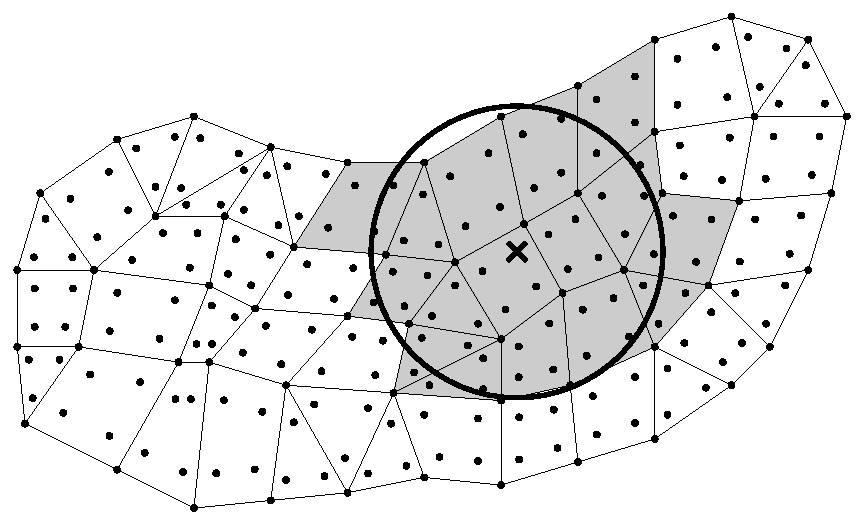
\includegraphics[width=0.7\textwidth]{pics/ApproxSQ.pdf}
    }
    \caption{Квадратурная аппроксимация области нелокального влияния}\label{fig:ApproxSQ}
\end{figure}

Ассемблирование остальных слагаемых уравнения теплопроводности (\ref{eq:ThermalSLAE}) происходит без каких-либо особенностей, поэтому просто выпишем их без подробного разъяснения деталей
\begin{gather}
	\label{eq:HeatTransferMatrix}
	\widehat{\textbf{K}}^{\alpha}_T =
	\sum\limits_{e \in \Gamma_h}
	\sum\limits_{n,m \in I^{e}}
	\sum\limits_{q \in Q^e}
	w_q \alpha N_n^e (\boldsymbol{x}_q) N_m^e (\boldsymbol{x}_q) J_q^e \boldsymbol{E}_n \otimes \boldsymbol{E}_m,
	\\
	\label{eq:HeatTransferVector}
	\textbf{T}^{\alpha} =
	\sum\limits_{e \in \Gamma_h}
	\sum\limits_{n \in I^{e}}
	\sum\limits_{q \in Q^e}
	w_q \alpha N_n^e (\boldsymbol{x}_q) T_{\alpha} (\boldsymbol{x}_q) J_q^e \boldsymbol{E}_n,
	\\
	\label{eq:InnerFlux}
	\textbf{Q} =
	\sum\limits_{e \in S_h}
	\sum\limits_{n \in I^e}
	\sum\limits_{q \in Q^e}
	w_q q_V (\boldsymbol{x}_q) J_q^e \boldsymbol{E}_n,
	\\
	\label{eq:OuterFlux}
	\textbf{F} =
	\sum\limits_{e \in \Gamma_h}
	\sum\limits_{n \in I^e}
	\sum\limits_{q \in Q^e}
	w_q f (\boldsymbol{x}_q) J_q^e \boldsymbol{E}_n.
\end{gather}
Аналогично запишем ассемблирование остальных слагаемых и для уравнения равновесия (\ref{eq:StressSLAE})
\begin{gather}
	\label{eq:InnerPressure}
	\widehat{\textbf{B}} =
	\sum\limits_{e \in S_h}
	\sum\limits_{n \in I^e}
	\sum\limits_{q \in Q^e}
	w_q \boldsymbol{b} (\boldsymbol{x}_q) J_q^e \boldsymbol{E}_n,
	\\
	\label{eq:OuterPressure}
	\widehat{\textbf{P}} = 
	\sum\limits_{e \in \Gamma_h}
	\sum\limits_{n \in I^e}
	\sum\limits_{q \in Q^e}
	w_q \boldsymbol{p} (\boldsymbol{x}_q) J_q^e \boldsymbol{E}_n,
	\\
	\label{eq:LocalThermalExpansion}
	\widehat{\textbf{E}}^L = 
	\sum\limits_{e \in S_h}
	\sum\limits_{n \in I^e}
	\sum\limits_{q \in Q^e}
	w_q \nabla N_n^e (\boldsymbol{x}_q) \widehat{\mathbf{C}} \cdot \cdot \widehat{\boldsymbol{\alpha}} \Delta T (\boldsymbol{x}_q) J_q^e \boldsymbol{E}_n,
\end{gather}
\begin{multline}
	\label{eq:NonLocalThermalExpansion}
	\widehat{\textbf{E}}^{NL} = 
	\sum\limits_{e \in S_h}
	\sum\limits_{n \in I^e}
	\sum\limits_{q \in Q^e}
	w_q \nabla N_n^e (\boldsymbol{x}_q) J_q^e 
	\times \\ \times
	\sum\limits_{e' \in S_h^q}
	\sum\limits_{q' \in Q^{e'}}
	w_{q'} \varphi (\boldsymbol{x}_q, \boldsymbol{x}_{q'}) \widehat{\mathbf{C}} \cdot \cdot \widehat{\boldsymbol{\alpha}} \Delta T (\boldsymbol{x}_{q'}) J_{q'}^{e'} \boldsymbol{E}_n.
\end{multline}
Отметим, что при ассемблировании $\widehat{\textbf{E}}^{NL}$ был использован метод квадратурной аппроксимации области нелокального влияния $S'(\boldsymbol{x})$, который ранее применялся к матрицам нелокальной телопроводности и жёсткости (\ref{eq:ApproxNonloc}).

\section{Вычисление производных величин}\label{sec:NumericalMethods/FluxStressCalculating}

После решения СЛАУ (\ref{eq:ThermalSLAE}) и (\ref{eq:StressSLAE}) на основе полученных сеточных функций температуры $\textbf{T}$ и перемещения $\widehat{\textbf{U}}$ можем найти их производные величины, такие как вектор плотности теплового потока $\boldsymbol{q}$ и тензор напряжений $\widehat{\boldsymbol{\sigma}}$ соответственно. Для этого вычислим градиенты сеточных функций в квадратурных узлах пользуясь формулами (\ref{eq:ApproxTemperatureGradient}) и (\ref{eq:ApproxStrain}). Далее аппроксимируем интегралы (\ref{eq:BiotFourier}) и (\ref{eq:DuamelNeumann}), для этого снова воспользуемся процедурой квадратурной аппроксимации области нелокального влияния, после чего получаем формулы для вычисления вектора плотности теплового потока
\begin{gather}
	\label{eq:ApproxFlux}
	\boldsymbol{q}_q = 
	\left(	
	-p_1 \lambda T_m N^e_{m,k} (\boldsymbol{x}_q)
	-p_2 \sum\limits_{e' \in S_h^q} \sum\limits_{q' \in Q^{e'}} w_{q'} \lambda T_{m'} N^e_{m',k} (\boldsymbol{x}_{q'}) J^{e'}_{q'}
	\right) \boldsymbol{e}_k
\end{gather}
и тензора напряжений
\begin{multline}
	\label{eq:ApproxStress}
	\widehat{\boldsymbol{\sigma}}_q =
	\Biggr(
	p_1 C_{ijkl} \left(\varepsilon_{kl} (\boldsymbol{x}_q) - \alpha_{kl} \Delta T_q \right)
	+\\+
	p_2 \sum\limits_{e' \in S_h^q} \sum\limits_{q' \in Q^{e'}} w_{q'} C_{ijkl} \left(\varepsilon_{kl} (\boldsymbol{x}_{q'}) - \alpha_{kl} \Delta T_{q'} \right) J^{e'}_{q'}
	\Biggr) \boldsymbol{e}_k \otimes \boldsymbol{e}_l,
\end{multline}
где $\boldsymbol{q}_q$, $\widehat{\boldsymbol{\sigma}}_q$ и $\Delta T_q$ --- значения вектора плотности теплового потока, тензора напряжений и разницы температур в квадратурном узле $q$ соответственно.

Для дальнейшего анализа полученных решений переинтерполируем их из квадратурных узлов в регулярные узлы сетки. Для этого при рассмотрении конкретного узла сетки определим ближайшие квадратурные узлы каждого из элементов, в состав которых входит этот узел, после чего вычислим среднюю величину с учётом площадей элементов. Другими словами, вначале для каждого элемента необходимо решить задачу минимизации с поиском нужного индекса $q^e$
\begin{gather*}
	\min_{e \in E^n} \rho(\boldsymbol{x}_n, \boldsymbol{x}_q) \rightarrow q^e,
	\quad
	n \in S_h
\end{gather*}
где $E^n$ --- множество элементов, которым принадлежит узел $n$. После чего проводим процедуру осреднения с весами, где в качестве весовых множителей используем площади элементов
\begin{gather*}
	|S^n| = \sum\limits_{e \in E^n} |S^e|,
	\quad
	\boldsymbol{q}_n = \sum\limits_{e \in E^n} \dfrac{\boldsymbol{q}_{q^e} |S^e|}{|S^n|},
	\quad
	\widehat{\boldsymbol{\sigma}}_n = \sum\limits_{e \in E^n} \dfrac{\widehat{\boldsymbol{\sigma}}_{q^e} |S^e|}{|S^n|},
\end{gather*}
где $\boldsymbol{q}_n$ и $\widehat{\boldsymbol{\sigma}}_n$ --- значения плотности теплового потока и напряжений в регулярных узлах сетки соответственно.
\chapter{Реализация программного комплекса}\label{ch:ProgramComplex}

\section{Общая структура программного комплекса}\label{sec:ProgramComplex/GeneralStructure}

В рамках диссертационной работы был реализован конечно-элементный программный комплекс NonLocFEM \cite{NonLocFEM}. Основная задача комплекса --- эффективное решение термомеханических задач в нелокальных постановках на современных вычислительных системах с использованием технологий параллельных вычислений OpenMP \cite{OpenMP} и MPI \cite{MPI}. Все описанные далее методы и алгоритмы реализованы в рамках данного комплекса, а именно: аппроксимация области нелокального влияния; параллельные алгоритмы ассемблирования конечно-элементных матриц; алгоритмы балансировки данных между процессами и потоками исполнения; интегрирование с использованием нестандартных базисов конечных элементов; решатели СЛАУ с использованием специально разработанных предобуславливателей; а также многие другие алгоритмы и методы, на которых не будем заострять слишком много внимания.

Глобальная структура программного комплекса включает в себя математическое ядро и обработчик конфигурационных файлов. Математическое ядро, в свою очередь, также состоит из нескольких взаимосвязанных библиотек, где в качестве основных можно выделить следующие: metamath, parallel, mesh и solvers. В них находятся необходимые примитивы и алгоритмы для конечно-элементных расчётов. Обработчик конфигурационных файлов работает со структурами, представленными в формате JSON \cite{JSONShema} и на их основе формирует запросы для математического ядра, которое проводит необходимые расчёты и возвращает результаты в форматах, которые можно прочитать популярными программами для визуализации данных, например Paraview \cite{Paraview}. Помимо собственных разработок в зависимости комплекса входят две сторонние библиотеки: библиотека линейной алгебры Eigen~\cite{EigenLib} и библиотека для работы со структурами в формате JSON N.~Lohmann~\cite{NlohmannJson}. Схема взаимосвязи модулей программы представлена на Рис.~\ref{pic:NonLocFEMSchema}, где зависимый модуль указывает стрелкой на модуль от которого он зависит.

\begin{figure}[ht]
    \centerfloat{
        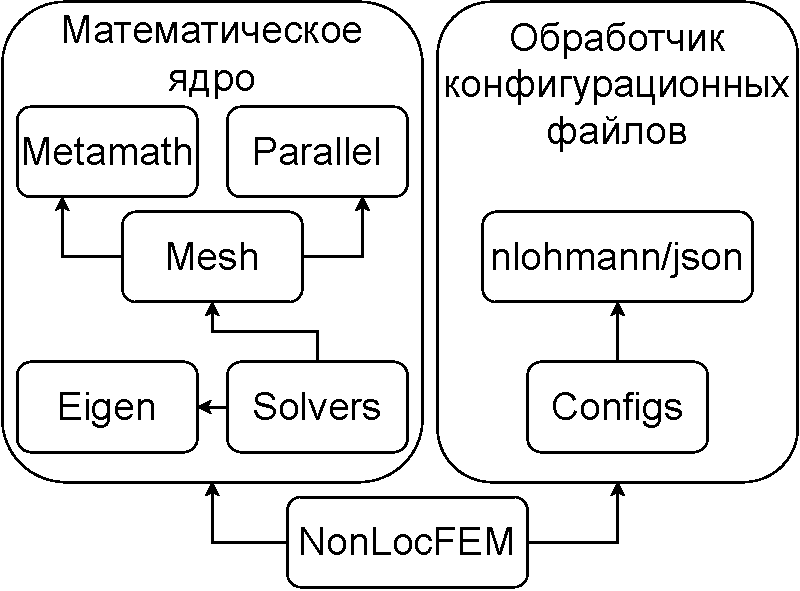
\includegraphics[width=0.7\textwidth]{pics/NonLocFEMSchema.pdf}
    }
    \caption{Структура программы NonLocFEM}\label{pic:NonLocFEMSchema}
\end{figure}

Программный комплекс NonLocFEM реализован на языке программирования C++ \cite{CppReference}. Выбор в пользу этого языка был обоснован его популярностью, богатой стандартной библиотекой, а главное производительностью итоговых программ. Помимо этого, язык предоставляет широкий спектр возможностей в реализации своих идей, особенно если говорить про актуальный на сегодняшний день стандарт языка C++23, возможности которого повсеместно использованы в программном комплексе. Язык C++ мультипарадигменный, поэтому в нём существует возможность совмещать объектно-ориентированные и функциональные подходы к программированию. Объектно-ориентированный подход выражен в виде возможности создания достаточно сложных иерархий классов, в которых могут быть использованы виртуальные методы. Это в свою очередь подразумевает позднее связывание кода программы, то есть во время работы программы могут быть использованы объекты с разной логикой обработки тех или иных данных, имея при этом общий интерфейс. Функциональная парадигма в контексте языка программирования C++ выражена в виде метапрограммирования шаблонов \cite{Alexandresku, Vandevoorde}, где часть вычислений можно вынести на этап компиляции программы, на основе результатов которых генерируется конечный исполняющий файл. Комбинирование двух парадигм открывает возможность совместить такие, порой несовместимые, аспекты программы, как гибкость исходного кода с его производительностью. А учитывая специфику вычислительных программ, в разработке программного комплекса NonLocFEM был сделан достаточно большой уклон в сторону функционых подходов метапрограммирования.

Особенно много приёмов метапрограммирования было использовано в библиотеке metamath, за счёт чего она и получила такое название. В этой библиотеке реализованы различные математические примитивы и функции, а также представлена адаптированная версия библиотеки символьного дифференцирования на этапе компиляции symdiff, основную концепцию которой можно найти в монографии Краснова~М.М.~\cite{KrasnovMeta}. Библиотека symdiff содержит в себе базовые примитивы: константа, переменная; базовые математические операции, такие как  сложение, вычитание, умножение, деление; ряд математических функций, включающих в себя экспоненту, логарифм, тригонометрические функции и многие другие. Благодаря этим примитивам можно строить выражения любой сложности, каждое из которых образует уникальный тип данных. Все эти типы данных объединяет общий интерфейс, предоставляющий возможность вычислить значение этого выражения в точке и посчитать его производную по заданной переменной, при этом вычисление производной порождает новый тип данных, который регистрируется на этапе компиляции программы и соотвествует выражению, являющейся производной исходного выражения. При этом были предприняты меры по оптимизации конечных выражений, сокращающих количество операций, которые необходимы при вычислении значения в точке.

На основе библиотеки symdiff, в рамках библиотеки metamath, была построена библиотека конечных элементов finite\_elements, в которой symdiff использована при описании базисных функций форм элементов и вычислении их производных компилятором. Такой подход значительно упрощает процесс добавления новых элементов, а также сокращает время отладки программы, так как большая часть ошибок, как правило, происходит именно при ручном дифференцировании базисов элементов. Помимо этого такой подход ещё сокращает исходный код программы, так как для добавления нового конечного элемента прикладному программисту необходимо всего лишь описать базис нового элемента в терминах библиотеки symdiff и записать координаты его узлов в локальной системе координат элемента. Для некоторых семейств элементов такой процесс можно автоматизировать, например, для семейства лагранжевых элементов, где базисы элементов построены по определённому алгоритму. Таким образом, можно указать порядок элемента, после чего компилятор сгенерирует необходимый базис в виде набора выражений, которые в дальнейшем могут быть им же и продифференцированы. Помимо дифференцирования базисов, в этой библиотеке также представлен функционал, связанный с процедурой интегрирования. Интегрирование, в отличие от дифференцирования, здесь реализовано численно. Библиотека содержит в себе наборы квадратур разного порядка, при помощи которых выполняется процедура интегрирования. Все элементы и квадратуры, описанные в рамках данной библиотеки, имеют единый интерфейс, поэтому дальнейшие конечно-элементные алгоритмы могут быть записаны в обобщённой форме.

Библиотека mesh предназначена для работы с конечно-элементными сетками. Основным классом данной библиотеки является класс хранилище, объекты которого могут читать файлы с сетками и представлять их в виде, с которым взаимодествуют алгоритмы программы, в том числе и алгоритмы модуля solvers. Схема хранения подразумевает, что элементы образованы путём перечисления номеров узлов, которые им принадлежат, а также ссылкой на объект библиотеки finite\_elements, в котором определены функции формы и квадратурные узлы в локальной системе координат элемента. Также в схеме хранения участвуют координаты узлов сетки и именованные группы элементов, образующих подобласти для определения границ, на которых далее можно задать разные граничные условия. Также было принято решение о том, что в случае использования распределённых вычислений при помощи библиотеки MPI, сетка представлена целиком на каждом отдельном процессе выполнения программы. Такое решение связано с желанием не усложнять схему хранения, ведь для задач в нелокальных постановках, как правило, используются достаточно грубые сетки, содержащие малое количество элементов.

Помимо класса хранилища, в библиотеке mesh также реализованы алгоритмы для работы с конечно-элеметными сетками. Здесь реализованы алгоритмы вычисления квадратурных узлов в глобальной системе координат, вычисления в них якобианов и производных функций форм относительно глобальных переменных. Здесь реализован шаблонный параллельный алгоритм обхода по сетке, на базе которого построены алгоритмы балансировки данных, алгоритм перенумерации узлов Катхилла --- Макки, алгоритм аппроксимации области нелокального влияния и алгоритмы формирования и заполнения портрета конечно-элеметных матриц из модуля solvers. Также в библиотеке mesh реализован функционал сохранения результатов расчётов.

В библиотеке solvers находятся обобщённые алгоритмы ассемблирования матриц и правых частей, и решатели СЛАУ.

Продолжая обзор библиотек программы следует поговорить о библиотеке parallel. Во многом эта библиотека является <<обёрткой>> над библиотеками параллельного программирования OMP и MPI. Она служит двум основным принципам: во-первых, осовременить и обобщить интерфейсы давно устовшихся функций из ранее упомянутых библиотек, которые в современном C++ выглядят весьма громоздко, а во-вторых, собрать все параллельные вызовы в одном месте, что позволяет легко отключать параллелилизм без дополнительных сложностей связанных с компиляцией программы. Кроме того эта библиотека содержит в себе алгоритмы балансировок данных и удобные примитивы для работы с параллельным кодом.

Для связи структур описанных в формате JSON с математическим ядром была разработана библиотека configs. Она содержит в себе примитивы, которые вычисляются на основе JSON и интерпретируются конечной программой в терминах представленных в математическом ядре программы. В случае несоответствия структуры описанной в JSON с ожидаемой библиотека генерирует сообщения об ошибках с указанием места в конфигурационном файле, где возникла эта ошибка.

Для переносимости кода были использованы такие инструменты, как пакетный менеджер Conan \cite{Conan} и система автоматизации сборки \mbox{CMake \cite{CMake}.} Данные инструменты являются кроссплатформенными и распространяются бесплатно, что позволяет легко переносить проект с компьютера на компьютер, а также обеспечивает гибкость в выборе версий сторонних библиотек и настройке компиляции \mbox{проекта.}

\section{Параллельный алгоритм ассемблирования матриц}\label{sec:ProgramComplex/ParallelAlgorithm}

Задачи в нелокальных постановках обладают достаточно большой вычислительной сложностью. Матрицы, получаемые после конечно-элементной аппроксимации, значительно более плотные по сравнению с их классическими аналогами, а также требуют огромных вычислительных ресурсов для их ассемблирования \cite{AMCSM2019}. Поэтому возникает спрос на использование всех возможностей современных компьютеров, а именно параллельные вычисления на машинах с общей и распределённой памятью. Но для того, чтобы полностью задействовать все вычислительные ресурсы, необходимо разработать алгоритм пригодный для распараллеливания.

Для начала упростим аппроксимацию области нелокального влияния $S'(\boldsymbol{x})$, так как рассматриваемый ранее способ квадратурной аппроксимации, описанный формулой (\ref{eq:ApproxNonloc}) и представленный на Рис.~\ref{fig:ApproxSQ}, крайне неудобен для практической реализации. Поэтому возникает идея упростить его и проводить аппроксимацию не относительно квадратурных узлов сетки, а относительно центров элементов. На Рис.~\ref{fig:ApproxSE} крестом обозначен центр элемента относительно которого проводится аппроксимация, область нелокального влияния ограничена окружностью, точками обозначены центры элементов, а серым цветом выделены элементы образующие аппроксимированную область нелокального влияния $S_h^e$. Такой способ аппроксимации будем называть элеметной аппроксимацией. Тогда в алгоритме ассемблирования нелокальной матрицы (\ref{eq:ApproxNonloc}) сможем поменять местами знаки суммирования, после чего сможем преобразовать его к следующему виду
\begin{gather}
	\label{eq:ApproxNonlocByElem}
	\widehat{\textbf{K}}^{NL}_{\mathcal{F}} =
	\sum\limits_{e \in S_h}
	\sum\limits_{n \in I^e}
	\sum\limits_{e' \in S_h^e}
	\sum\limits_{m \in I^{e'}}
	\sum\limits_{q \in Q^e}
	w_q J_q^e
	\sum\limits_{q' \in Q^{e'}}
	w_{q'} \varphi(\boldsymbol{x}_q, \boldsymbol{x}_{q'}) 
	\textbf{K}_{nm}^{e e'}(\boldsymbol{x}_q, \boldsymbol{x}_{q'}) J_{q'}^{e'}.
\end{gather}
Также можем упростить и алгоритм вычисления нелокального температурного линейного расширения (\ref{eq:NonLocalThermalExpansion}) 
\begin{gather}
	\label{eq:NonLocalThermalExpansionByElem}
	\widehat{\textbf{E}}^{NL} = 
	\sum\limits_{e \in S_h}
	\sum\limits_{n \in I^e}
	\sum\limits_{e' \in S_h^e}
	\sum\limits_{q \in Q^e}
	w_q \nabla N_n^e (\boldsymbol{x}_q) J_q^e
	\sum\limits_{q' \in Q^{e'}}
	w_{q'} \varphi (\boldsymbol{x}_q, \boldsymbol{x}_{q'}) \widehat{\mathbf{C}} \cdot \cdot \widehat{\boldsymbol{\alpha}} \Delta T (\boldsymbol{x}_{q'}) J_{q'}^{e'} \boldsymbol{E}_n.
\end{gather}

\begin{figure}[ht]
    \centerfloat{
        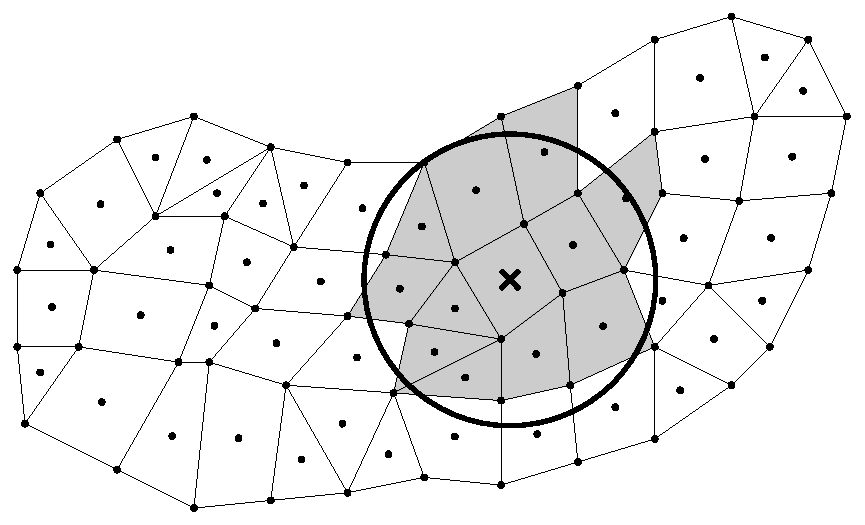
\includegraphics[width=0.7\textwidth]{pics/ApproxSE.pdf}
    }
    \caption{Элементная аппроксимация области нелокального влияния}\label{fig:ApproxSE}
\end{figure}

Такой подход позволяет отделить алгоритм обхода по сетке, ответственного за формирование портрета матрицы, от алгоритма интегрирования, однако, он обладает дефектом, который заключается в том, что не все квадратурные узлы, попадающие в область $S'(\boldsymbol{x}_q)$, центр которой находится в некотором квадратурном узле под номером $q$, попадают под покрытие аппроксимированной области нелокального влияния $S_h^e$. Это может приводить к нарушениям баланса, что в свою очередь приводит к менее точному решению и даже осциляциям. Для решения данной проблемы, радиус поиска соседних элементов нужно брать больше радиуса нелокальности $r$, например, на величину максимального расстояния между центрами двух смежных элементов, где под смежными элементами подразумеваем элементы обладающие хотя бы одним общим узлом. Таким образом, все необходимые квадратурные узлы будут учтены в расчёте.

После разделения алгоритма обхода сетки и алгоритма интегрирования, можем изменить первый таким образом, чтобы сделать его пригодным для параллельных вычислений. Главной проблемой алгоритма (\ref{eq:ApproxNonlocByElem}) остаётся зависимость номера узла сетки от номера текущего элемента из-за чего при использовании параллельных вычислений существует вероятность возникновения гонки данных, что, в зависимости от подхода к распараллеливанию, может приводить к неправильному решению задачи, или частым барьерным синхронизациям, которые в свою очередь снижают эффективность использования параллельных вычислений. Поэтому возникает идея изменить порядок суммирования таким образом, чтобы такой зависимости не было. Для этого определим для каждого узла сетки $n \in S_h$ множество элементов $E^n$, которым он принадлежит и изменим порядок суммирования так, чтобы под первым знаком суммы были номера узлов, а под вторым номера элементов которым он принадлежит
\begin{gather}
	\label{eq:ApproxNonlocParallel}
	\widehat{\textbf{K}}^{NL}_{\mathcal{F}} =
	\sum\limits_{n \in S_h}
	\sum\limits_{e \in E^n}
	\sum\limits_{e' \in S_h^e}
	\sum\limits_{m \in I^{e'}}
	\sum\limits_{q \in Q^e}
	w_q J_q^e
	\sum\limits_{q' \in Q^{e'}}
	w_{q'} \varphi(\boldsymbol{x}_q, \boldsymbol{x}_{q'}) 
	\textbf{K}_{nm}^{e e'}(\boldsymbol{x}_q, \boldsymbol{x}_{q'}) J_{q'}^{e'}.
\end{gather}
Такой алгоритм сборки матрицы является построчным, соответственно каждую строку матрицы можно собирать независимо в своём исполняемом потоке, а также распределить вычисление строк между вычислительными узлами.

Полученный алгоритм (\ref{eq:ApproxNonlocParallel}) пригоден для параллельных вычислений на машинах с общей и распределённой памятью, однако, возникает проблема балансировки данных и объёма вычислений. При решении этих проблем стоит начинать с проблемы балансировки данных, так как из-за неё есть вероятность возникновения ситуации, когда задача не может быть решена, в силу того, что на одном из вычислительных узлов может не хватить оперативной памяти, в то время как при балансировке данных такой проблемы можно было бы избежать.

При балансировке данных будем исходить из гипотезы, что на каждом вычислительном узле $p \in P$ установлено одинаковое количество оперативной памяти и данные нужно распределить равномерно между всеми вычислительными узлами $P$. Для этого необходимо найти общее число элементов матрицы $M$, затем найти среднее $M_m = M / |P|$ и распределить строки матрицы между вычислительными узлами таким образом, чтобы в каждой группе строк количество элементов матрицы было приблизительно равным $M_p \approx M_m$. На практике удобнее всего брать группы последовательных строк. Причём при балансировке нет необходимости формировать полный портрет матрицы, это также можно делать построчно, что гораздо эффективнее и легко реализовать. Также при балансировке необходимо учесть симметрию полученной матрицы, так как из-за достаточно больших объёмов выгодно хранить лишь её половину.

После балансировки данных между вычислительными узлами, можем также провести балансировку объёмов вычислений между вычислительными потоками. Для этого необходимо проделать ту же процедуру, что и при балансировке данных, но осреднять не по количеству элементов матрицы, а по количеству вызовов функции интегрирования. В некоторых ситуациях такая балансировка может быть полезна и между вычислительными узлами, например, когда сборка матрицы занимает гораздо больше времени, чем решение итоговой СЛАУ.

Вместе с параллельным алгоритмом ассемблирования нелокальных матриц (\ref{eq:ApproxNonlocParallel}), можем также выписать параллельный алгоритм ассемблирования локальных матриц (\ref{eq:LocalMatrix})
\begin{gather*}
	\widehat{\textbf{K}}^L_{\mathcal{F}} =
	\sum\limits_{n \in S_h}
	\sum\limits_{e \in E^n}
	\sum\limits_{m \in I^e}
	\sum\limits_{q \in Q^e}
	w_q \textbf{K}^{ee}_{nm} (\boldsymbol{x}_q, \boldsymbol{x}_q) J_q^e,
\end{gather*}
Аналогично можно поступить и с ассемблированием матрицы теплообмена (\ref{eq:HeatTransferMatrix}), а также векторами в правой части (\ref{eq:HeatTransferVector}) --- (\ref{eq:OuterFlux}) уравнения теплопроводности (\ref{eq:ThermalSLAE})
\begin{gather*}
	\textbf{Q} =
	\sum\limits_{n \in S_h}
	\sum\limits_{e \in E^n}
	\sum\limits_{q \in Q^e}
	w_q q_V (\boldsymbol{x}_q) J_q^e \boldsymbol{E}_n,
\end{gather*}
\begin{gather*}
	\textbf{F} =
	\sum\limits_{n \in \Gamma_h}
	\sum\limits_{e \in E^n}
	\sum\limits_{q \in Q^e}
	w_q f (\boldsymbol{x}_q) J_q^e \boldsymbol{E}_n,
\end{gather*}
\begin{gather*}
	\widehat{\textbf{K}}^{\alpha}_T =
	\sum\limits_{n \in \Gamma_h}
	\sum\limits_{e \in E^n}
	\sum\limits_{m \in I^{e}}
	\sum\limits_{q \in Q^e}
	w_q \alpha N_n^e (\boldsymbol{x}_q) N_m^e (\boldsymbol{x}_q) J_q^e \boldsymbol{E}_n \otimes \boldsymbol{E}_m,
\end{gather*}
\begin{gather*}
	\textbf{T}^{\alpha} =
	\sum\limits_{n \in \Gamma_h}
	\sum\limits_{e \in E^n}
	\sum\limits_{q \in Q^e}
	w_q \alpha N_n^e (\boldsymbol{x}_q) T_{\alpha} (\boldsymbol{x}_q) J_q^e \boldsymbol{E}_n.
\end{gather*}
Проделаем те же выкладки и для векторов правой части (\ref{eq:InnerPressure}) --- (\ref{eq:LocalThermalExpansion}) и (\ref{eq:NonLocalThermalExpansionByElem}) уравнения равновесия (\ref{eq:StressSLAE})
\begin{gather*}
	\widehat{\textbf{B}} =
	\sum\limits_{n \in S_h}
	\sum\limits_{e \in E^n}
	\sum\limits_{q \in Q^e}
	w_q \boldsymbol{b} (\boldsymbol{x}_q) J_q^e \boldsymbol{E}_n,
\end{gather*}
\begin{gather*}
	\widehat{\textbf{P}} = 
	\sum\limits_{e \in \Gamma_h}
	\sum\limits_{n \in I^e}
	\sum\limits_{q \in Q^e}
	w_q \boldsymbol{p} (\boldsymbol{x}_q) J_q^e \boldsymbol{E}_n,
\end{gather*}
\begin{gather*}
	\widehat{\textbf{E}}^L = 
	\sum\limits_{n \in S_h}
	\sum\limits_{e \in E^n}
	\sum\limits_{q \in Q^e}
	w_q \nabla N_n^e (\boldsymbol{x}_q) \cdot \widehat{\mathbf{C}} \cdot \cdot \widehat{\boldsymbol{\alpha}} \Delta T (\boldsymbol{x}_q) J_q^e \boldsymbol{E}_n,
\end{gather*}
\begin{gather*}
	\widehat{\textbf{E}}^{NL} = 
	\sum\limits_{n \in S_h}
	\sum\limits_{e \in E^n}
	\sum\limits_{e' \in S_h^e}
	\sum\limits_{q \in Q^e}
	w_q \nabla N_n^e (\boldsymbol{x}_q) J_q^e \cdot
	\sum\limits_{q' \in Q^{e'}}
	w_{q'} \varphi (\boldsymbol{x}_q, \boldsymbol{x}_{q'}) \widehat{\mathbf{C}} \cdot \cdot \widehat{\boldsymbol{\alpha}} \Delta T (\boldsymbol{x}_{q'}) J_{q'}^{e'} \boldsymbol{E}_n,
\end{gather*}
Отметим, что при ассемблировании векторов на каждом вычислительном узле можем также ограничиться только теми строками, которые были получены при балансировке.

\section{Алгоритм аппроксимации области нелокального влияния}\label{sec:ProgramComplex/SearchMeighbours}

При аппроксимации области нелокального влияния необходимо использовать метод поиска ближайших соседей, однако, важно выбрать оптимальный для рассматриваемых задач алгоритм. Наивный алгоритм линейного поиска имеет квадратичную сложность $O (N^2)$, в связи с чем на достаточно подробных сетках время поиска может быть весьма существенным. Поэтому построим алгоритм поиска в основе которого лежит k-d дерево \cite{kdtree}.

Суть метода на основе k-d дерева заключается в разделении пространства занимаемого телом на равномерные ячейки, после разбиения на которые необходимо составить списки узлов соответствующие ячейкам, в которых они оказались. Размер ячеек следует брать равным радиусу поиска, тогда при поиске ближайших соседей поиск можно ограничить до ячейки в которой находится этот узел и смежных ей ячейкам. В качестве алгоритма поиска внутри ячеек можно использовать обычный линейный поиск, тогда сложность такого алгоритма можно оценить как $O(N \log N)$, что на подробных сетках заметно быстрее линейного поиска. Пример разбиения представлен на Рис. \ref{fig:SearchNeighbours}, где крестом указан рассматриваемый узел, тёмно-серым цветом выделена ячейка, которой принадлежит этот узел, а светло-серым смежные ей ячейки, область нелокального влияния ограничена окружностью.

\begin{figure}[ht]
    \centerfloat{
        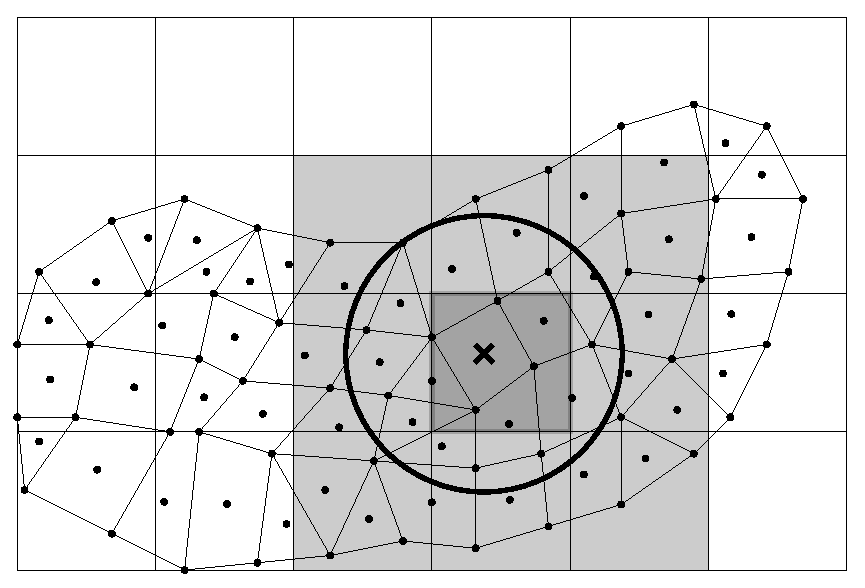
\includegraphics[width=0.7\textwidth]{pics/SearchNeighbours.pdf}
    }
    \caption{K-d дерево для поиска ближайших соседей}\label{fig:SearchNeighbours}
\end{figure}

\section{Оптимизация базисных функций конечных элементов}\label{sec:ProgramComplex/BasisOptimization}

Помимо эффективных алгоритмов сборки матрицы жёсткости, также возникает потребность в эффективном решении итоговых СЛАУ. Прямые методы, применённые к разреженным матрицам, как правило требуют значительных затрат оперативной памяти, поэтому возникает спрос на использование итерационных методов решения \cite{Demmel}. Однако итерационные методы могут иметь слишком медленную сходимость, которая в первую очередь обусловлена самой системой. Таким образом возникает идея уменьшить число обусловленности системы и как правило для этого используют разного рода предобуславливатели и адаптируют сетку таким образом, чтобы элементы были ближе к своим исходным формам \cite{MeshOptimization1, MeshOptimization2}. Также для ускорения сходимости можно подобрать начальные данные, чтобы они были как можно точнее к искомому решению. Но в случае, когда для вычислений используют элементы высшего порядка, появляется дополнительная возможность оптимизировать базис элемента под конкретную задачу.

Обычно использование элементов высшего порядка может быть связано с желанием более точно аппроксимировать искомые величины или производные от этих величин, такие как тепловые потоки или деформации \cite{HighOrderElements1, HighOrderElements2}. Также они могут понадобиться для решения специфических задач, где могут встречаться производные высшего порядка. В задачах не обладающих такой спецификой большой популярностью обладают квадратичные серендиповые элементы, так как они позволяют достаточно точно аппроксимировать градиенты искомых функций и при этом, как показано на Рис.~\ref{fig:QuadraticSerendipity}, не имеют внутренних узлов, что заметно упрощает расчёты.

\begin{figure}[ht]
    \centerfloat{
        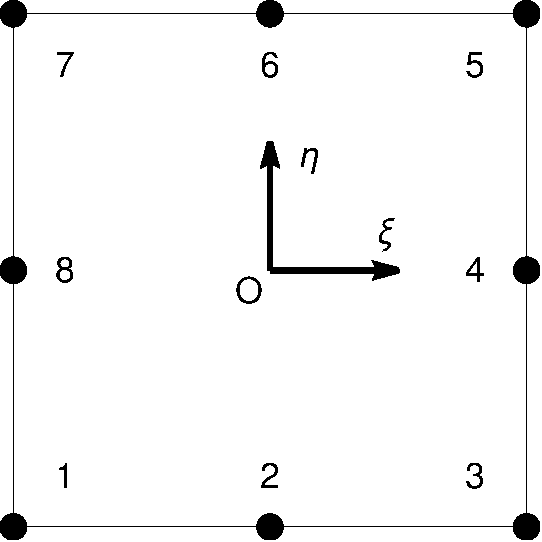
\includegraphics[width=0.5\textwidth]{pics/QuadraticSerendipity.pdf}
    }
    \caption{Квадратичный серендиповый элемент в локальной системе координат $\text{O}\xi\eta$}\label{fig:QuadraticSerendipity}
\end{figure}

Набор базисных функций для квадратичного серендипового элемента, которые предложил O.~Zienkiewicz \cite{Zienkiewicz}, не единственный и к тому же обладает рядом дефектов, которые повышают число обусловленности итоговой системы уравнений. Поэтому рассмотрим семейство базисных функций с дополнительным параметром $s$ \cite{QuadraticSerensipity}
\begin{gather*}
    N_i = \dfrac{1}{16} (1 + \xi_i \xi) (1 + \eta_i \eta) ((9s - 1) (1 - \xi_i \xi - \eta_i \eta) + (9s + 3) \xi_i \xi \eta_i \eta), \\ 
    i = 1, 3, 5, 7; \xi_i, \eta_i = \pm 1, \\
    N_i = \dfrac{1}{16} (1 - \xi^2) (1 + \eta_i \eta) ((5 - 9s) + (9s + 3)\eta_i \eta),
    \quad
    i = 2, 6; \ \eta_i = \pm 1, \\
    N_i = \dfrac{1}{16} (1 - \eta^2) (1 + \xi_i \xi) ((5 - 9s) + (9s + 3)\xi_i \xi),
    \quad
    i = 4, 8; \ \xi_i = \pm 1.
\end{gather*}
Выбор параметра $s$ был основан на следующих предположениях
\begin{gather*}
    \int\limits_{-1}^{1} \int\limits_{-1}^{1} N_i (\xi, \eta) d\xi d\eta = s,
    \quad
    i = 1, 3, 5, 7, \\
    \int\limits_{-1}^{1} \int\limits_{-1}^{1} N_i (\xi, \eta) d\xi d\eta = 1 - s,
    \quad
    i = 2, 4, 6, 8.
\end{gather*}
Таким образом, классический базис можно получить при $s = -1 / 3$.

Теперь можем перейти к задаче минимизации числа обусловленности матриц теплопроводности $\widehat{\textbf{K}}_T$ и жёсткости $\widehat{\textbf{K}}_E$, которые для удобства дальнейшего изложения будем обозначать одной буквой $\widehat{\textbf{K}}$. Для этого введём понятие числа обусловленности, как квадратный корень отношения максимального по модулю собственного числа $\lambda_{\max}$ к минимальному по модулю собственному числу $\lambda_{\min}$ матрицы $\widehat{\textbf{K}}$
\begin{gather}
	\label{eq:CondValue}
	\operatorname{cond} \widehat{\textbf{K}} = \sqrt{\dfrac{|\lambda_{\max}|}{|\lambda_{\min}|}}.
\end{gather}

Воспользуемся гипотезой, что минимальное по модулю собственное число $\lambda_{min}$ слабо зависит от параметров модели и дополнительного параметра базиса. Так как след матрицы равен сумме её собственных значений, а сама матрица симметричная и положительно определённая, то задача минимизации числа обусловленности эквивалентна задаче минимизации следа матрицы
\begin{gather*}
    \min\limits_s \operatorname{tr} \widehat{\mathbf{K}} =
    \min\limits_s \sum\limits_{e \in S_h} \int\limits_{S^e} \sum\limits_{i = 0}^k \sum\limits_{j = 0}^2 c_{j} N^e_{i,j} d S^e,
\end{gather*}
где $k$ --- количество функций форм элемента, $c_{j}$ --- некоторые постоянные коэффициенты, зависящие от свойств материала. Но, как легко заметить, результат задачи оптимизации не зависит от количества элементов и их геометрических свойств (считаем, что сетка состоит из однородных элементов), поэтому можем упростить задачу и рассмотреть лишь один элемент в локальной системе координат. Таким образом, для квадратичного серендипового элемента задача оптимизации сводится к поиску минимума квадратичной параболы
\begin{gather}
	\label{eq:ParamSOptimal}
	\min\limits_s \int\limits_{-1}^{1} \int\limits_{-1}^{1} \sum\limits_{i = 0}^8 \sum\limits_{j = 0}^2 c_{j} N_{i, j}^2(\xi, \eta) d\xi d\eta =
	\min\limits_s C (27 s^2 -12 s + 19) \
	\rightarrow \ s = \dfrac{2}{9},
\end{gather}
где $C$ --- некоторая константа. Исходя из полученной оценки, ожидаемый минимум числа обусловленности, а также наибольшая скорость сходимости итерационных методов решения СЛАУ должна быть в окрестности точки $s = 2/9$.
\chapter{Анализ результатов расчётов}\label{ch:ResultsAnalysis} 

\section{Стратегия исследования и обезразмеривание}\label{sec:ResultsAnalysis/Strategy}

В дальнейших расчётах, для изучения качественных различий между классической (локальной) и нелокальной моделями, проведём процедуру обезразмеривания основных расчётых параметров уравнений теплопроводности (\ref{eq:StationaryHeatEquation}) и равновесия (\ref{eq:EquilibriumEquation}), где безразмерные параметры будем обозначать теми же символами, но с чертой над ними
\begin{gather*}
	\overline{\boldsymbol{x}} = \dfrac{\boldsymbol{x}}{L},
	\quad
	\overline{T} = \dfrac{T}{T_0},
	\quad
	\overline{\boldsymbol{\lambda}} = \dfrac{\widehat{\boldsymbol{\lambda}}}{\lambda_0},
	\quad
	\overline{E} = \dfrac{E}{\sigma_0},
	\quad
	\overline{\alpha}^T = \alpha^T T_0.
\end{gather*}
Здесь $L$ --- характерный размер области; $T_0$ --- нормализующий множитель для температуры; $\lambda_0$ --- нормализующий множитель для тензора теплопроводности; $\sigma_0$~---~нормализующий множитель для напряжений. Также чертой сверху будем обозначать безразмерные величины, которые образуются посредством комбинации приведённых выше безразмерных параметров. В расчётах, если не оговорено иначе, примем безразмерный тензор теплопроводности $\overline{\boldsymbol{\lambda}} = \widehat{\textbf{I}}_2$, безразмерный модуль Юнга $\overline{E} = 400$, коэффициент Пуассона $\nu = 0.3$ и безразмерный температурный коэффициент линейного расширения $\overline{\alpha}^T = 2.5 \cdot 10^{-3}$.

Стратегия исследования модели подразумевает вариацию основных параметров при фиксации всех остальных. Весовой параметр $p_1$ и радиус нелокальности $\overline{r}$ будем варьировать линейно, причём для параметра $p_1$ будут рассмотрены четыре сценария: отсутствие нелокальных эффектов ($p_1 = 1$); локальное слагаемое преобладает над нелокальным ($p_1 = 0.75$); локальное и нелокальное слагаемые имеют одинаковый вес ($p_1 = 0.5$); и нелокальное слагаемое преобладает над локальным ($p_1 = 0.25$). Полностью нелокальную постановку ($p_1 = 0$) рассматривать не будем, так как это приводит к некорректно поставленным краевым задачам, что требует дополнительных рассуждений при их решении.

Все дальнейшие расчёты будем проводить с использованием квадратичных серендиповых элементов, где характерный размер элемента будет указан отдельно для каждой решаемой задачи. Также, по возможности, для наглядности все расчётные параметры модели будут указаны прямо на рисунках с решениями. С целью уменьшения дублирования полученных выводов, некоторые промежуточные результаты будут учтены при решении последующих задач.

\section{Основные особенности решений}\label{sec:ResultsAnalysis/KeyFeatures}

Рассмотрим изучение нелокальных моделей теплопроводности и упругости с решения серии задач на единичном квадрате $S = \left\{ \overline{\boldsymbol{x}} \ | \ -0.5 \leqslant \overline{x}_1, \overline{x}_2 \leqslant 0.5 \right\}$. Решения будем искать на равномерной сетке $S_h$ с характерным размером элементов $h = 0.004$. Поставим граничные и интегральное условия для уравнения теплопроводности
\begin{gather*}
	\boldsymbol{n} \cdot \overline{\boldsymbol{q}} |_{\overline{x}_1 = -0.5} = 1,
	\quad
	\boldsymbol{n} \cdot \overline{\boldsymbol{q}} |_{\overline{x}_1 = 0.5} = -1,
	\quad
	\int\limits_S T dS = 0,
\end{gather*}
а также сформулируем граничные и геометрические условия для уравнения равновесия
\begin{gather*}
	n_j \overline{\sigma}_{j1} |_{\overline{x}_1 = -0.5} = -1,
	\quad
	n_j \overline{\sigma}_{j1} |_{\overline{x}_1 = 0.5} = 1,
	\quad
	\overline{u}_1 |_{\overline{x}_1 = 0} = 0,
	\quad
	\overline{u}_2 |_{\overline{x}_2 = 0} = 0.
\end{gather*}

Для определения относительного отклонения будем рассматривать нормированную разность нелокального и локального решений в сечениях вдоль оси нагружения, где в качестве нормировочного множителя будет выступать максимальное по модулю значение локального решения
\begin{gather*}
	\widetilde{T} = \dfrac{\overline{T}^{NL} - \overline{T}^L}{\max\limits_{\boldsymbol{x} \in S} \left| \overline{T}^L \right|},
	\quad
	\widetilde{u}_1 = \dfrac{\overline{u}^{NL}_1 - \overline{u}^L_1}{\max\limits_{\boldsymbol{x} \in S} \left| \overline{u}^L_1 \right|}.
\end{gather*}
Сравнительный анализ для уравнения теплопроводности и равновесия будем проводить одновременно, так как наблюдаемые в решениях явления весьма похожи.

Начнём изучение решений с вариации весового параметра модели $p_1$. Как показано на Рис.~\ref{fig:VariationP1}, увеличение вклада нелокального влияния увеличивает отклонение решений относительно классического. Причём при параметре $p_1 = 0.25$ наблюдаем осциляции решения вблизи границ области, где также наблюдаем кромочный эффект, характеризующийся резкими изменениями решения.

\begin{figure}[ht]
    \begin{minipage}[b][][b]{0.49\linewidth}\centering
        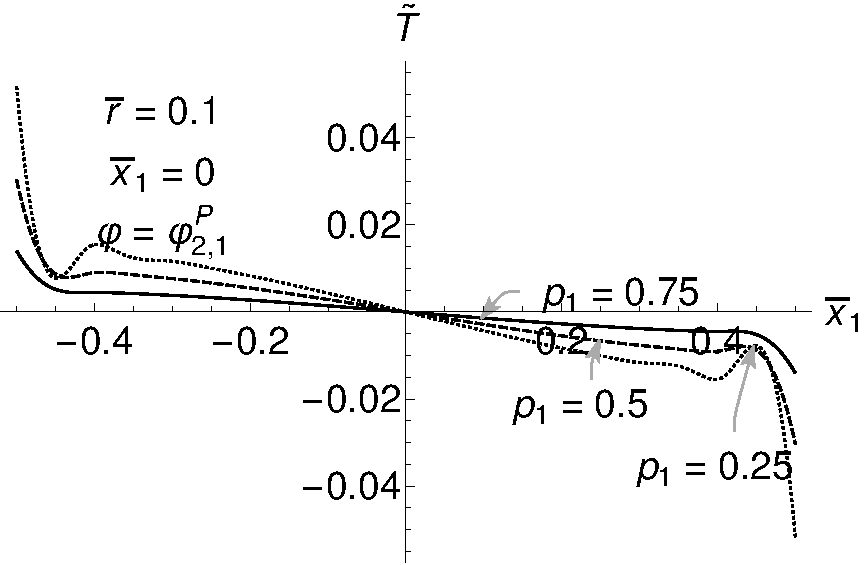
\includegraphics[width=\linewidth]{pics/TVarP1.pdf} \\ а)
    \end{minipage}
    \hfill
    \begin{minipage}[b][][b]{0.49\linewidth}\centering
        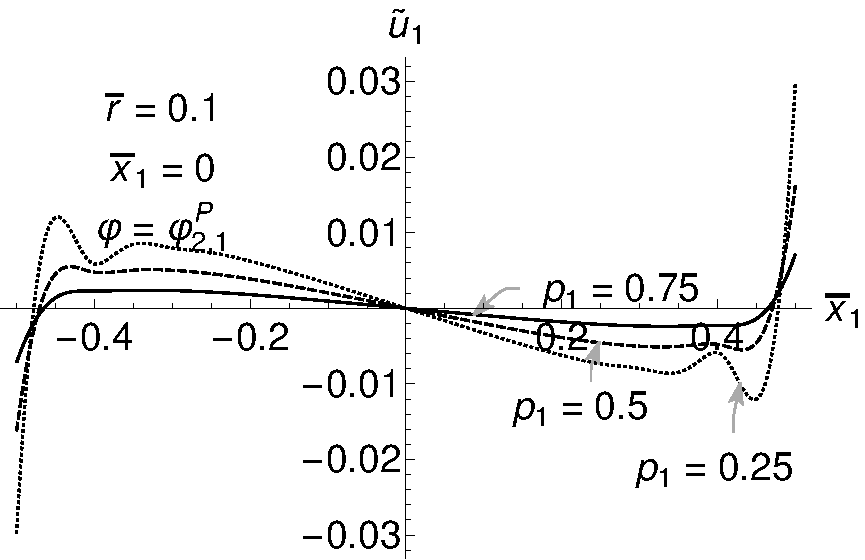
\includegraphics[width=\linewidth]{pics/U1VarP1.pdf} \\ б)
    \end{minipage}
    \caption{Решения при вариации весового параметра параметра $p_1$}
    \label{fig:VariationP1}
\end{figure}

Вариация радиуса нелокальности, представленная на Рис.~\ref{fig:VariationR}, также увеличивает отклонения, но вместе с тем и ширину кромочного эффекта пропорционально радиусу.

\begin{figure}[ht]
    \begin{minipage}[b][][b]{0.49\linewidth}\centering
        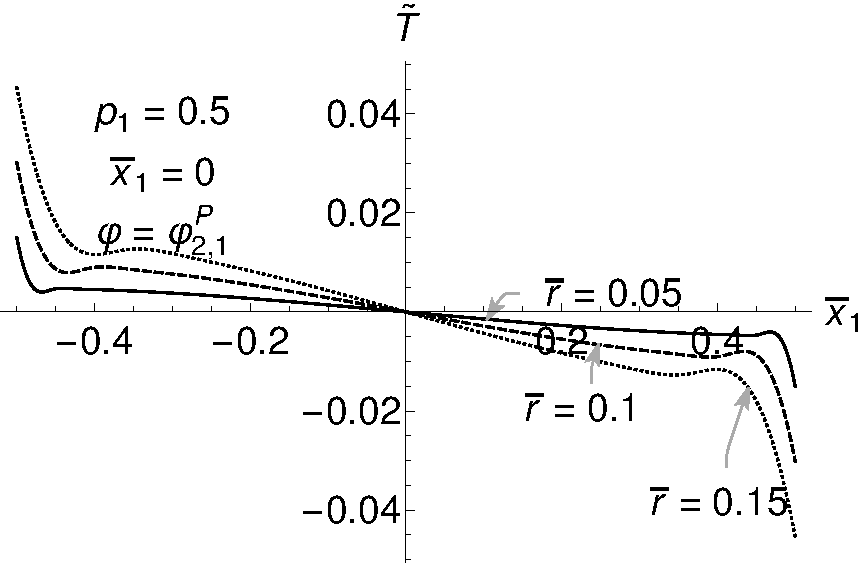
\includegraphics[width=\linewidth]{pics/TVarR.pdf} \\ а)
    \end{minipage}
    \hfill
    \begin{minipage}[b][][b]{0.49\linewidth}\centering
        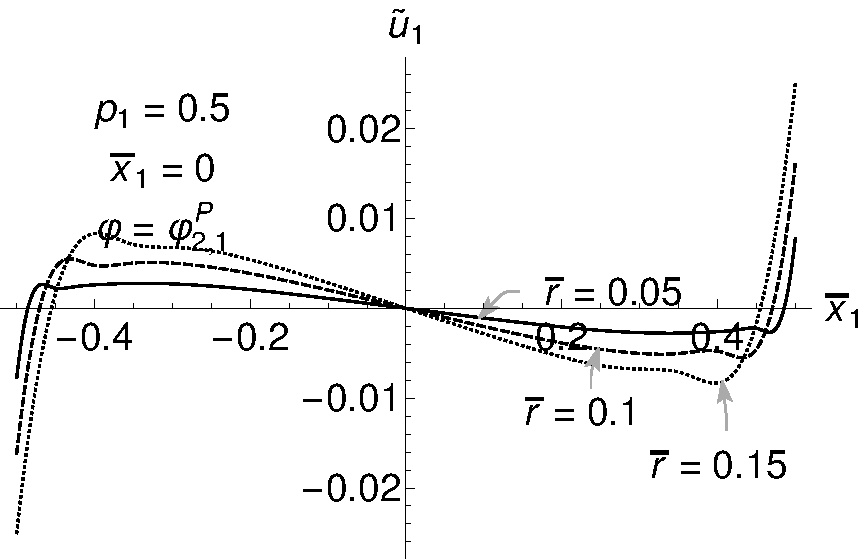
\includegraphics[width=\linewidth]{pics/U1VarR.pdf} \\ б)
    \end{minipage}
    \caption{Решения при вариации радиуса нелокальности $\overline{r}$}
    \label{fig:VariationR}
\end{figure}

Заметим, что в двумерном случае, отклонения также зависят и от рассматриваемого сечения. На Рис.~\ref{fig:VariationX2} представлены распределения температуры и перемещения в различных сечения и при приближении к свободным от условий границам отклонения возрастают, так как на них решение также подвержено кромочному эффекту. Наибольшие отклонения решений находятся в углах области, где кромочные эффекты двух границ складываются, и отклонения достигают 0.06 для уравнения теплопроводности и 0.15 для уравнения равновесия относительно классического решения при параметрах модели $p_1 = 0.5$ и $\overline{r} = 0.1$.

\begin{figure}[ht]
    \begin{minipage}[b][][b]{0.49\linewidth}\centering
        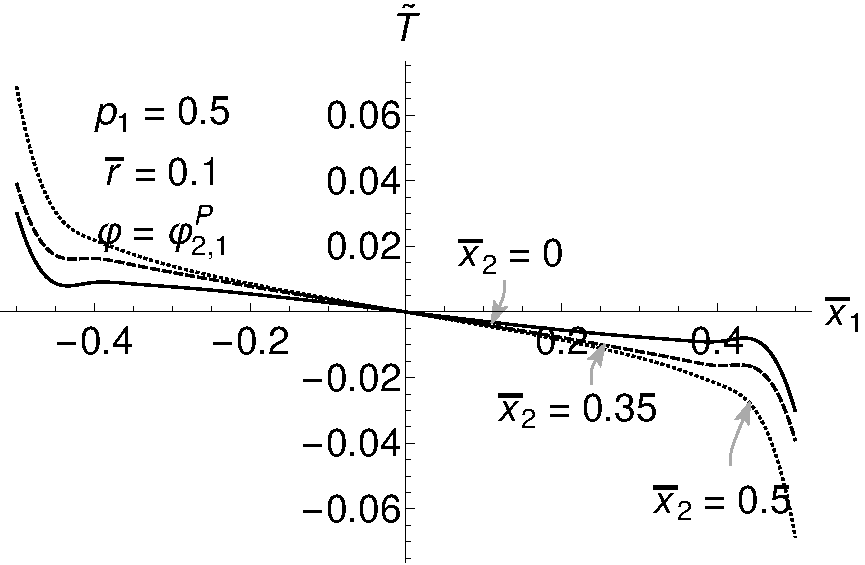
\includegraphics[width=\linewidth]{pics/TVarX2.pdf} \\ а)
    \end{minipage}
    \hfill
    \begin{minipage}[b][][b]{0.49\linewidth}\centering
        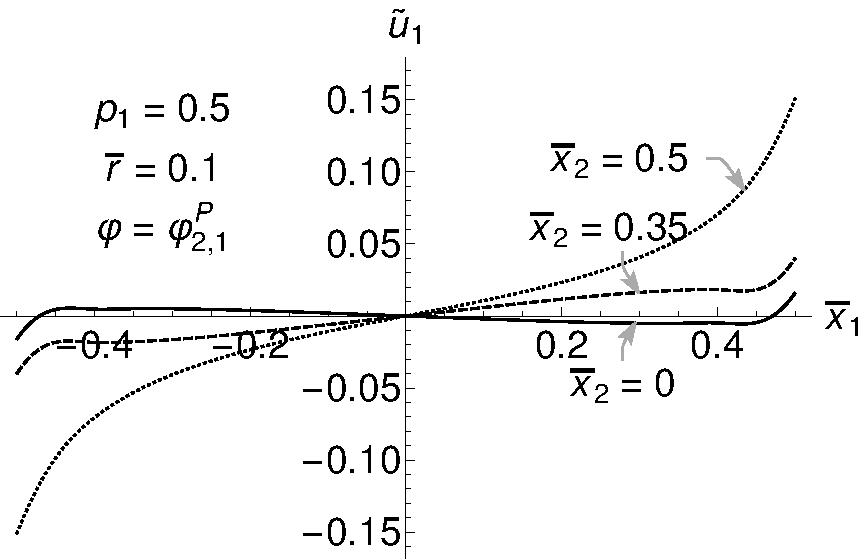
\includegraphics[width=\linewidth]{pics/U1VarX2.pdf} \\ б)
    \end{minipage}
    \caption{Нормированная разница решений в разных сечениях}
    \label{fig:VariationX2}
\end{figure}

Помимо уже рассмотренного, решения в нелокальной постановке также обладают и другими интересными особенностями. Например, в отличие от классического решения, компонента теплового потока $\overline{q}_2$ не равна нулю вблизи границ, где задан ненулевой тепловой поток, причём, как показано на Рис.~\ref{fig:Flux2}, решения обладают симметрией и также зависят от основных параметров модели. В отличие от температуры, увеличение радиуса нелокальности $\overline{r}$ не влияет на величину отклонений, но увеличивает размах кромочного эффекта, который здесь характеризуется увеличением площади областей, окружённых линиями уровней. Внутри области и на свободных от условий границах компонента плотности теплового потока $\overline{q}_2$ равна нулю.

\begin{figure}[ht]
    \begin{minipage}[b][][b]{0.49\linewidth}\centering
        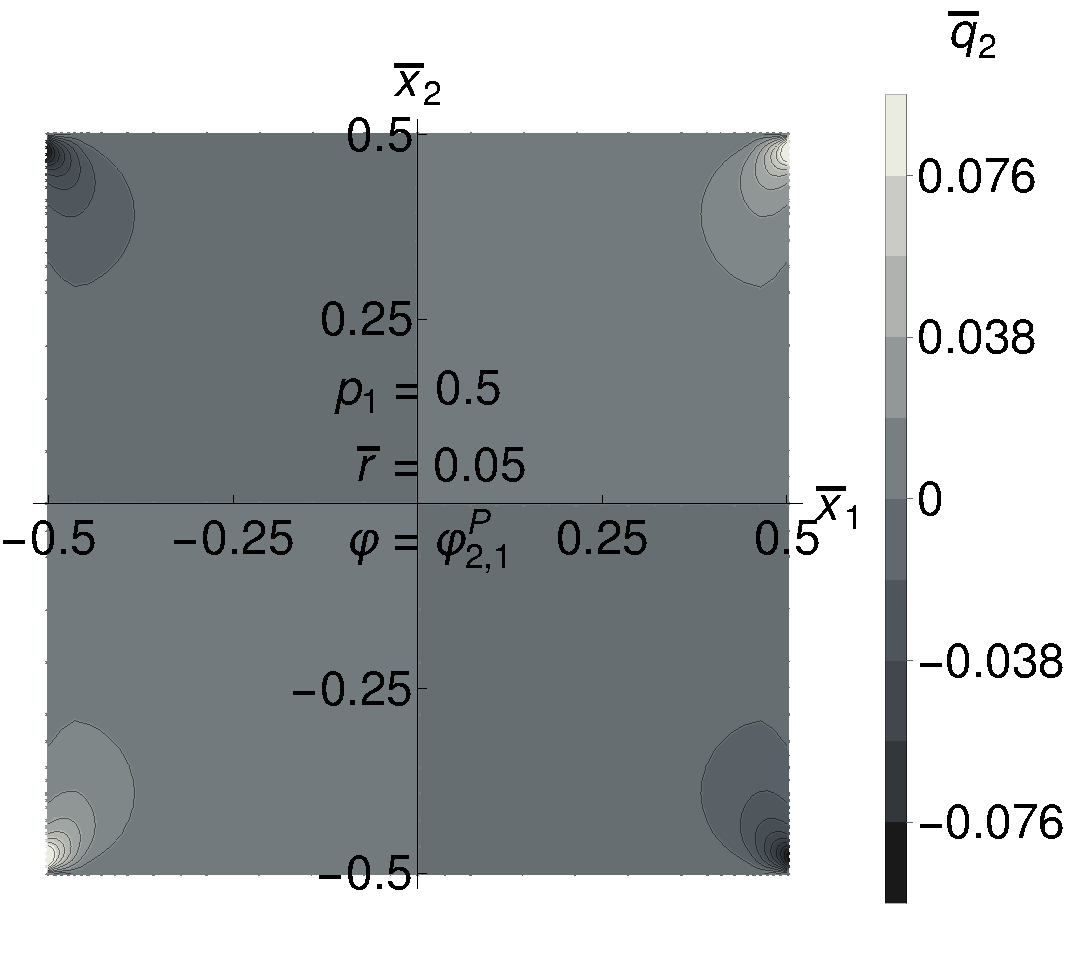
\includegraphics[width=\linewidth]{pics/Flux2R005.pdf} \\ а)
    \end{minipage}
    \hfill
    \begin{minipage}[b][][b]{0.49\linewidth}\centering
        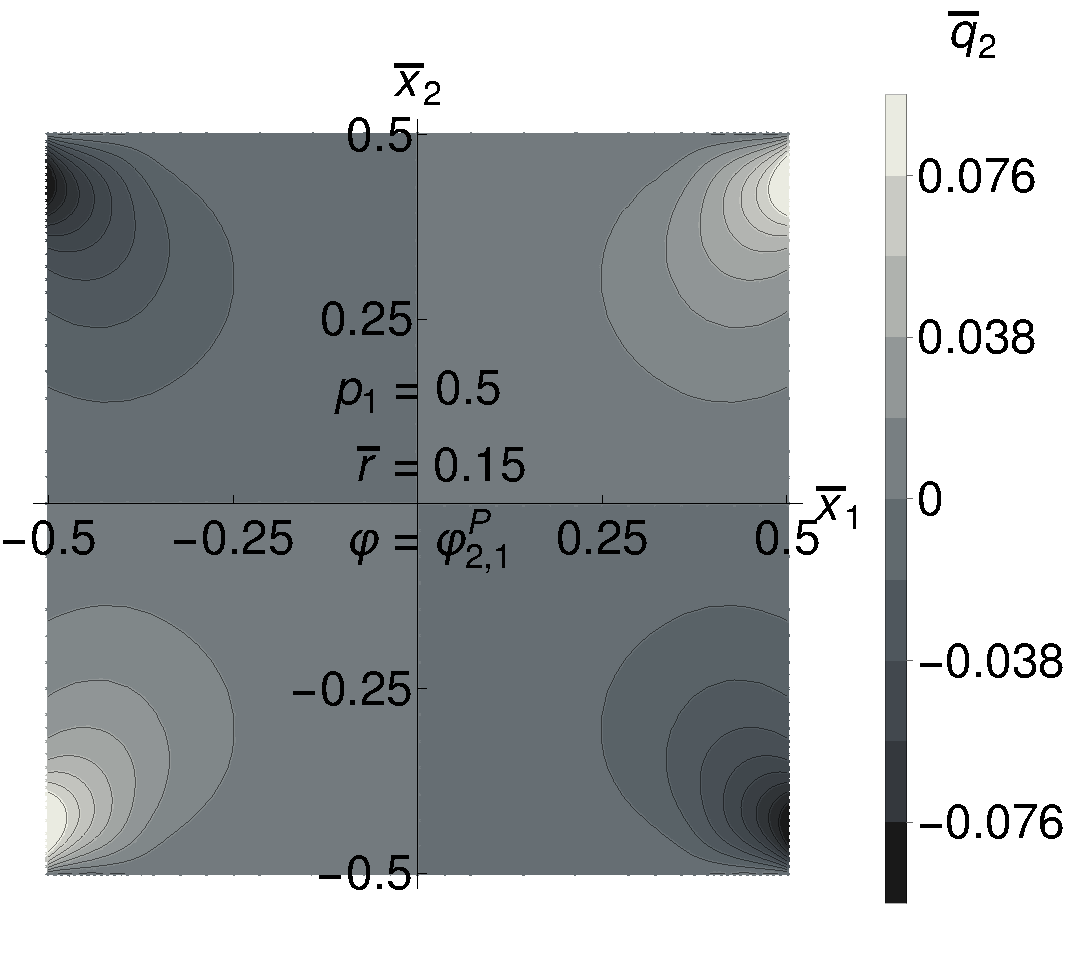
\includegraphics[width=\linewidth]{pics/Flux2R015.pdf} \\ б)
    \end{minipage}
    \caption{Распределение компоненты $\overline{q}_2$ при вариации $\overline{r}$}
    \label{fig:Flux2}
\end{figure}

Для уравнения равновесия в нелокальной постановке ненулевой становится компонента тензора напряжений $\overline{\sigma}_{12}$, а заодно и компонента тензора деформаций $\varepsilon_{12}$. Её распределение имеет более сложную, но при этом также симметричную форму и представлено на Рис.~\ref{fig:Sigma12}. Здесь, как и в случае с компонентой плотности теплового потока $\overline{q}_2$, вариация радиуса практически не оказывает влияния на максимальные значения напряжения и также увеличивает размах линий уровня. Отметим ещё, что на всех границах, включая те, где заданы нагружения, а также в центре области, значения $\overline{\sigma}_{12}$ равны нулю.

\begin{figure}[ht]
    \begin{minipage}[b][][b]{0.49\linewidth}\centering
        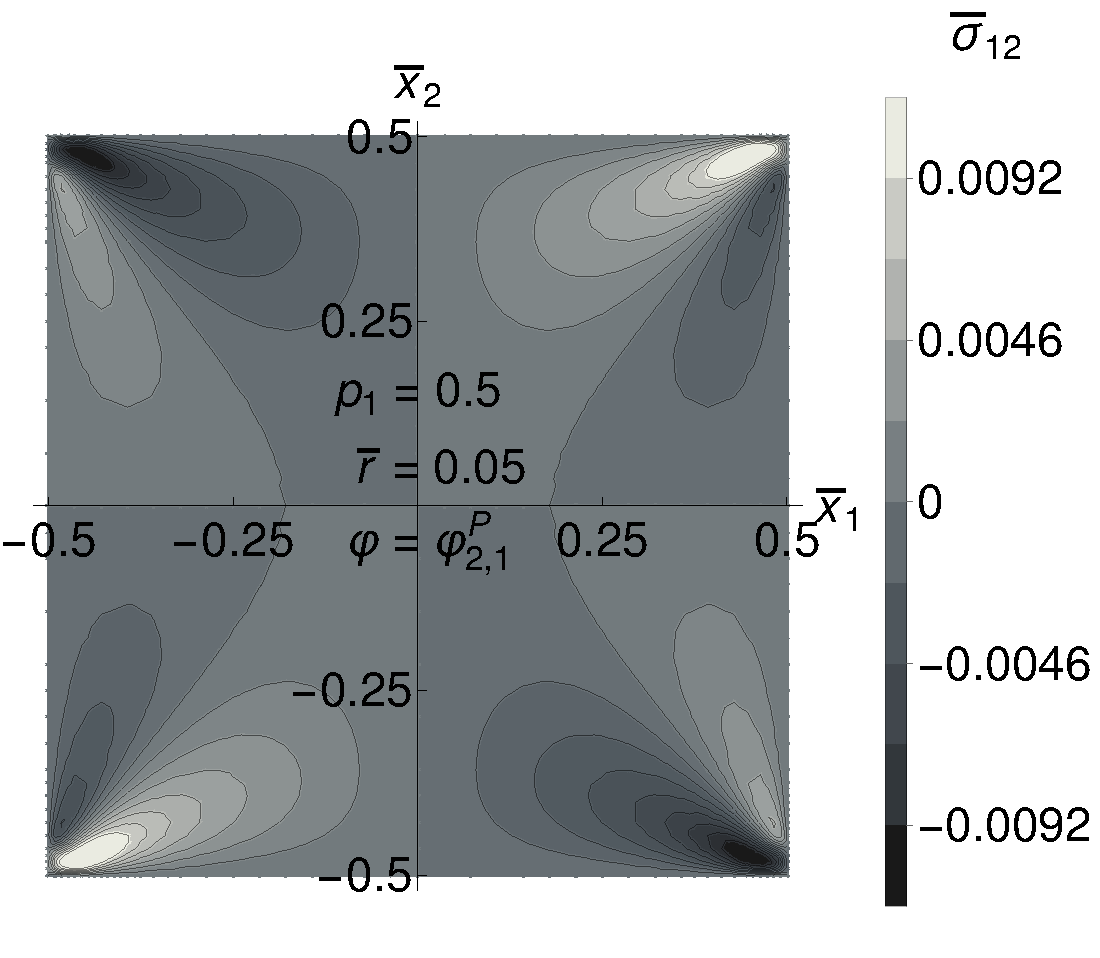
\includegraphics[width=\linewidth]{pics/Sigma12R005.pdf} \\ а)
    \end{minipage}
    \hfill
    \begin{minipage}[b][][b]{0.49\linewidth}\centering
        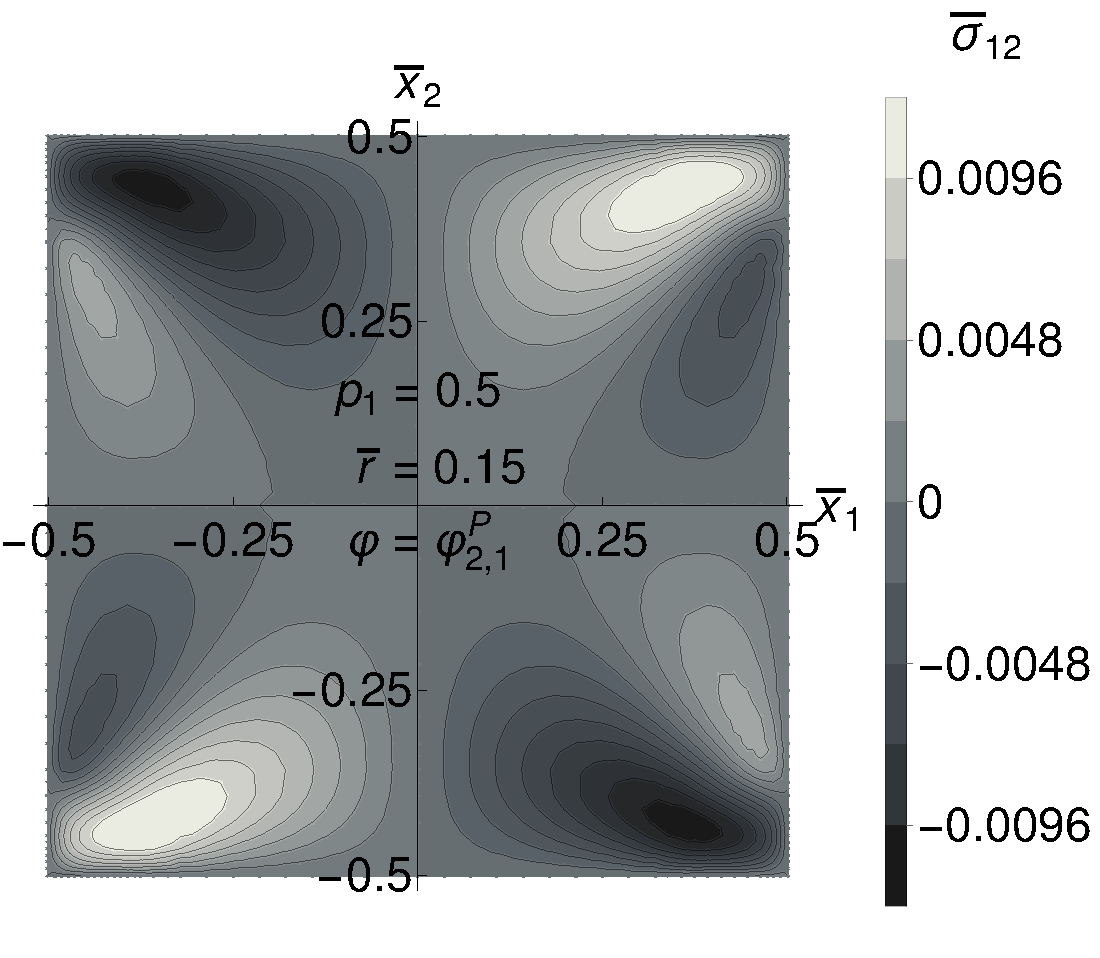
\includegraphics[width=\linewidth]{pics/Sigma12R015.pdf} \\ б)
    \end{minipage}
    \caption{Распределение компоненты $\overline{\sigma}_{12}$ при вариации $\overline{r}$}
    \label{fig:Sigma12}
\end{figure}

\section{Исследование функций нелокального влияния}\label{sec:ResultsAnalysis/KeyFeatures}

Изучим теперь влияние выбора функции нелокального влияния $\varphi$. Ранее уже были определены два параметрических семейства функций: полиномиальные $\varphi^P_{p,q}$ (\ref{eq:polynomialInfluence}) и экспоненциальные $\varphi^E_{p,q}$ (\ref{eq:exponentiallInfluence}). На их примере покажем как вариация основных параметров влияет на результаты решений. Не теряя общности исследования ограничимся решением только уравнения теплопроводности, но при этом будем сравнивать семейства функций между собой одновременно, так как их параметры, обозначенные одинаковыми символами, имеют одинаковый смысл. Рассматриваемую область и постановку задачи оставим той же, что уже была рассмотрена в предыдущем разделе.

Начнём исследование с вариации параметра $p$. Данный параметр отвечает за равномерность распределения функции влияния по заданной области $S'(\boldsymbol{x})$. Как показано на Рис.~\ref{fig:InfluenceVariationP}, отклонения решения растут вместе с параметром $p$ и достигают своего максимума, когда функция влияния вырождается в константу при $p \rightarrow \infty$. Здесь в качестве области нелокального влияния $S'(\overline{\boldsymbol{x}})$ был выбран круг с радиусом 0.1, поэтому для экспоненциального семейста функций был подобран и дисперсионный параметр нелокальности $\overline{r}$ при заданном квантиле $Q = 0.99$. Добавим ещё одно замечание, что для того, чтобы поведение экспоненциального семейства совпадало с полиномиальным, то есть увеличение параметра $p$ приводило к строгому увеличению отклонений, необходимо, чтобы параметр $p \geqslant n$.

\begin{figure}[ht]
    \begin{minipage}[b][][b]{0.49\linewidth}\centering
        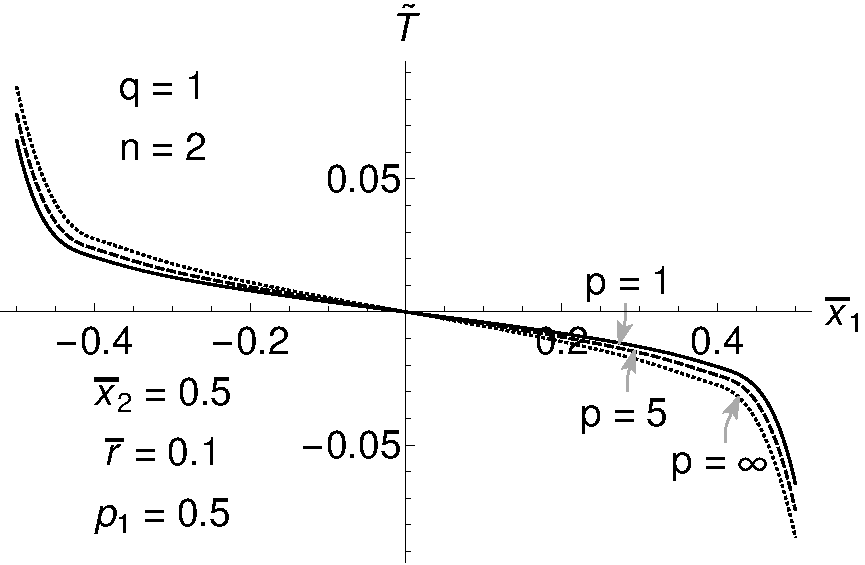
\includegraphics[width=\linewidth]{pics/TPolyInfluenceVariationP.pdf} \\ а)
    \end{minipage}
    \hfill
    \begin{minipage}[b][][b]{0.49\linewidth}\centering
        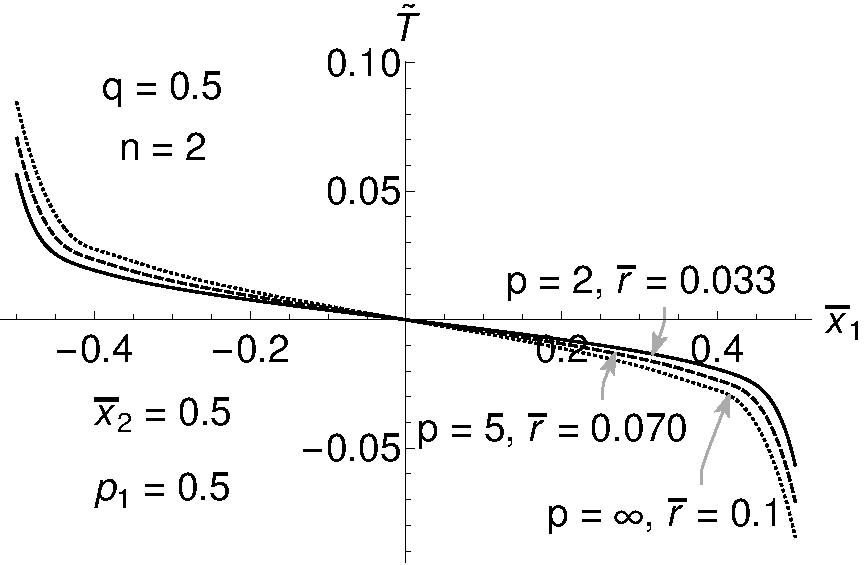
\includegraphics[width=\linewidth]{pics/TExpInfluenceVariationP.pdf} \\ б)
    \end{minipage}
    \caption{Вариация параметра $p$}
    \label{fig:InfluenceVariationP}
\end{figure}

Увеличение параметра $q$ концентрирует распределение функции нелокального влияния $\varphi$ в центре области $S'(\boldsymbol{x})$. Соответственно, при его увеличении отклонения решений относительно классического уменьшаются, что продемонстрировано на Рис.~\ref{fig:InfluenceVariationQ}. Здесь важно отметить, что для экспоненциальных функций дисперсионный параметр нелокальности $\overline{r}$ был выбран на основе функции с наименьшим значением параметра $q$, то есть для всех функций он совпадает. Сделано это по причине того, что данные параметры связаны между собой и если при изменении параметра $q$ подобрать подходящий под установленный квантиль $Q$ величину $\overline{r}$, распределения функций для всех $q$ будут совпадать.

\begin{figure}[ht]
    \begin{minipage}[b][][b]{0.49\linewidth}\centering
        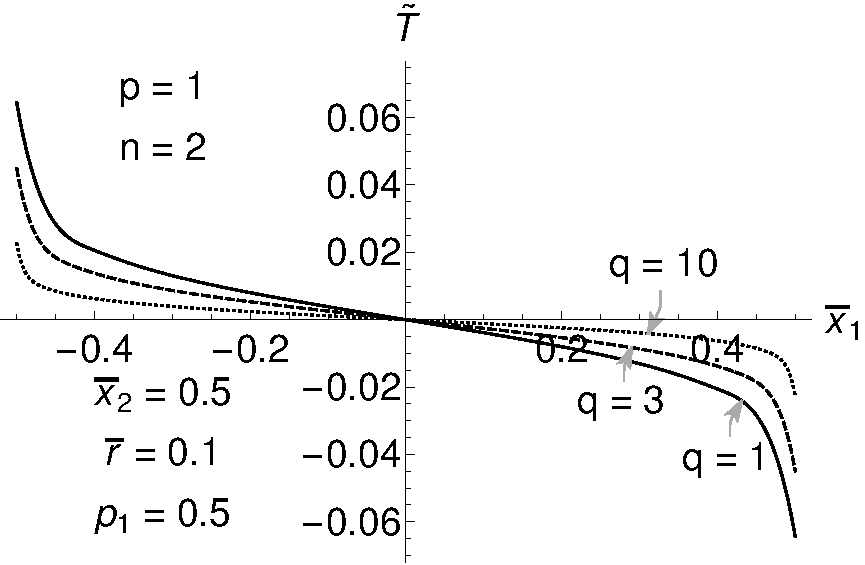
\includegraphics[width=\linewidth]{pics/TPolyInfluenceVariationQ.pdf} \\ а)
    \end{minipage}
    \hfill
    \begin{minipage}[b][][b]{0.49\linewidth}\centering
        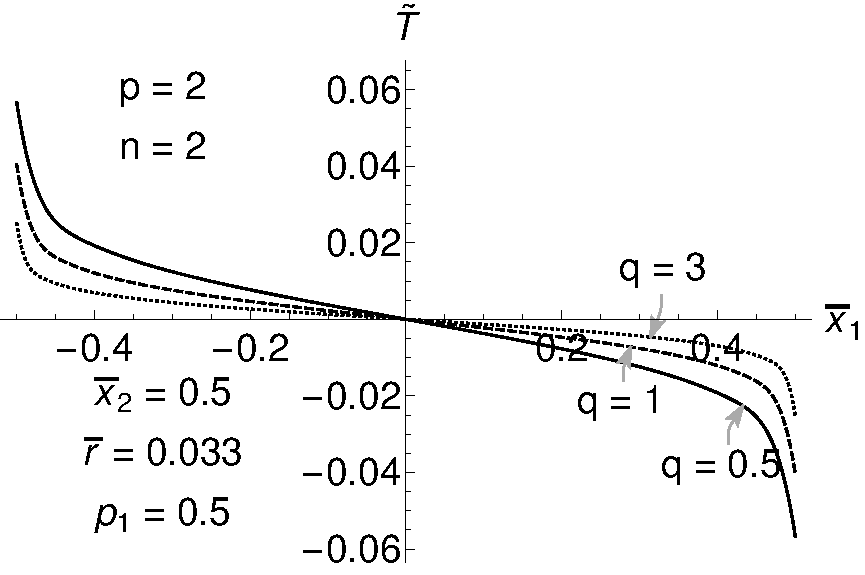
\includegraphics[width=\linewidth]{pics/TExpInfluenceVariationQ.pdf} \\ б)
    \end{minipage}
    \caption{Вариация параметра $q$}
    \label{fig:InfluenceVariationQ}
\end{figure}

Параметр $n$ является геометрическим, поэтому его изменение влияет на форму области $S'(\boldsymbol{x})$. Вместе с его увеличением увеличивается и покрываемая областью нелокального влияния площадь и, как показано на Рис.~\ref{fig:InfluenceVariationN}, отклонение решений. В силу независимости величины дисперсионного параметра $\overline{r}$ от параметра $n$ в уравнении (\ref{eq:quantil}), параметр $\overline{r}$ подбирался по правилу <<3 сигма>> на основе длины главной полуоси области $S'(\boldsymbol{x})$. Для экспоненциальных функций при заданных параметрах $p$ и $q$ влияние параметра $n$ становится несущественным, когда он больше $2$.

\begin{figure}[ht]
    \begin{minipage}[b][][b]{0.49\linewidth}\centering
        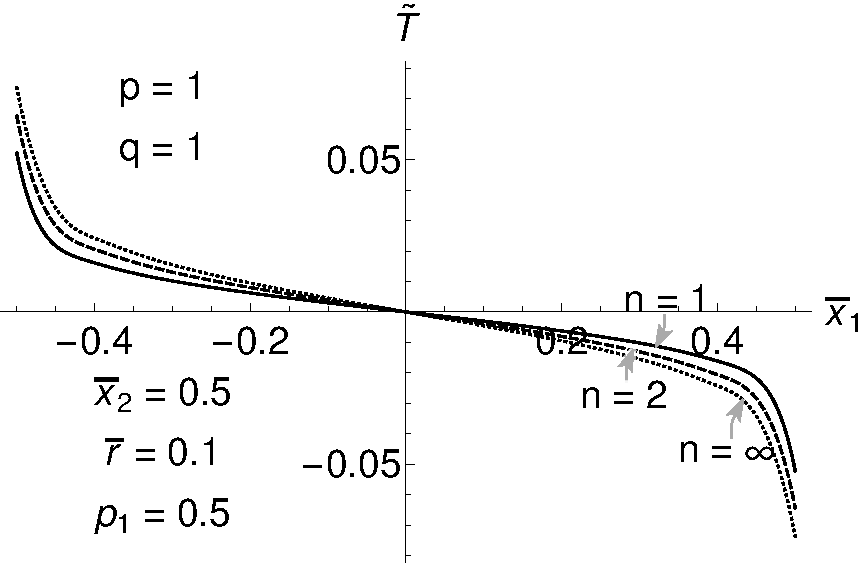
\includegraphics[width=\linewidth]{pics/TPolyInfluenceVariationN.pdf} \\ а)
    \end{minipage}
    \hfill
    \begin{minipage}[b][][b]{0.49\linewidth}\centering
        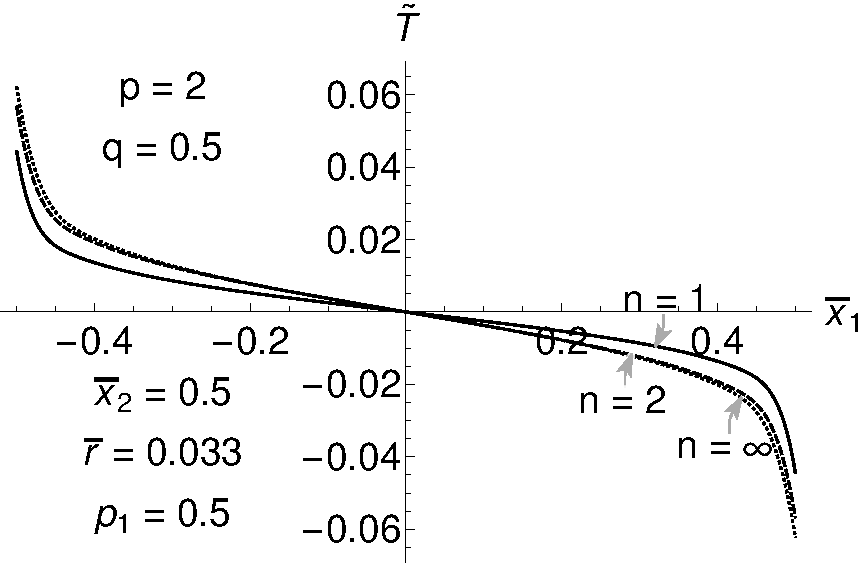
\includegraphics[width=\linewidth]{pics/TExpInfluenceVariationN.pdf} \\ б)
    \end{minipage}
    \caption{Вариация параметра $n$}
    \label{fig:InfluenceVariationN}
\end{figure}

Подведём некоторый промежуточный итог касательно выбора функции нелокального влияния $\varphi$. Было продемонстрировано, что её выбор может повлиять на степень отклонения решения, но качественных различий между решениями при различных параметрах функций нет. Также выбор семейства функций не оказывает существенного влияния на итоговые результаты. В связи с этими обстоятельствами, дальнейшие расчёты были проведены только с использованием квадратичных парабол $\varphi_{2,1}^P$ при $n = 2$, в силу того, что расчёты с использованием этой функции требуют наименьшего количества вычислительных ресурсов и этапы ассемблирования матрицы, вычисления тепловых потоков и напряжений происходят гораздо быстрее. Конечно, ещё меньше вычислительных операций требует функция $\varphi \equiv \text{const}$, но такая функция является предельной и не обладает свойством монотонного убывания из-за чего её использование формально является некорректным.

\section{Принципы Сен-Венана и стабильности теплового потока}\label{sec:ResultsAnalysis/SaintVenant}

Изучение свойств нелокальной теплопроводности и упругости следует начинать с простых задач, на примере которых можно исследовать основные принципы и положения присущие классическим моделям. К таким положениям можно отнести принцип стабильности теплового потока \cite{ThermalStability} и принцип Сен-Венана \cite{SaintVenant}, согласно которым любые интегрально эквивалентные возмущения поля являются локальными и вызывают одинаковые распределения поля вдали от точек приложения возмущения. В частности, для уравнения теплопроводности (\ref{eq:StationaryHeatEquation}) таким полем является поле плотности теплового потока $\boldsymbol{q}$, а для уравнения равновесия (\ref{eq:EquilibriumEquation}) --- поле \mbox{напряжений $\widehat{\boldsymbol{\sigma}}$.}

Для проверки этого высказывания проведём серию расчётов на прямоугольной области $S = \left\{ \boldsymbol{x} | -5 \leqslant x_1 \leqslant 5, -0.5 \leqslant x_2 \leqslant 0.5 \right\}$, с введённой на ней равномерной сеткой $S_h$ состоящей из $1500 \times 150$ элементов. Сформулируем граничные и интегральное условия для уравнения теплопроводности
\begin{gather*}
	\boldsymbol{n} \cdot \overline{\boldsymbol{q}} |_{\overline{x}_1 = -5} = f(\overline{x}_2),
	\quad
	\boldsymbol{n} \cdot \overline{\boldsymbol{q}} |_{\overline{x}_1 = 5} = -f(\overline{x}_2),
	\quad
	\iint\limits_S T dS = 0,
\end{gather*}
а также сформулируем граничные и геометрические условия для уравнения равновесия
\begin{gather*}
	n_j \overline{\sigma}_{j1} |_{\overline{x}_1 = -5} = -f(\overline{x}_2),
	\quad
	n_j \overline{\sigma}_{j1} |_{\overline{x}_1 = 5} = f(\overline{x}_2),
	\quad
	\overline{u}_1 |_{\overline{x}_1 = 0} = 0,
	\quad
	\overline{u}_2 |_{\overline{x}_2 = 0} = 0,
\end{gather*}
где $f$ --- функция задающая возмущение поля. Будем рассматривать три интегрально эквивалентных варианта возмущения
\begin{gather*}
	f_1 (x) = 1,
	\quad
	f_2 (x) = 2 - 4 |x|,
	\quad
	f_3 (x) = 4 |x|,
\end{gather*}
приложение которых, в виде теплового потока и давления заданных на левой и правой границах области $S$, изображено на Рис.~\ref{fig:SaintVenantLoads}.

\begin{figure}[ht]
    \begin{minipage}[b][][b]{0.49\linewidth}\centering
        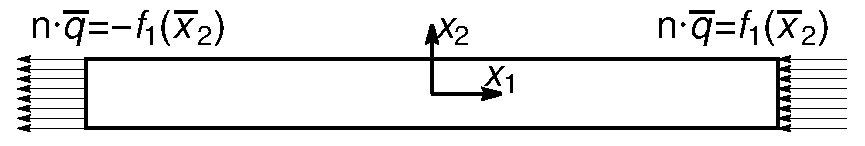
\includegraphics[width=\linewidth]{pics/RectangleFluxF1.pdf} \\ а)
        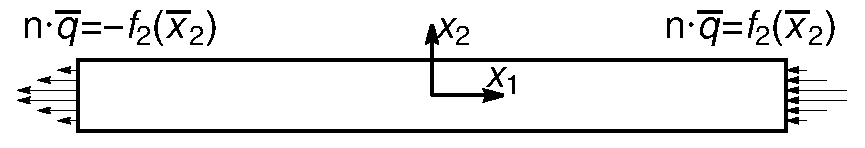
\includegraphics[width=\linewidth]{pics/RectangleFluxF2.pdf} \\ в)
        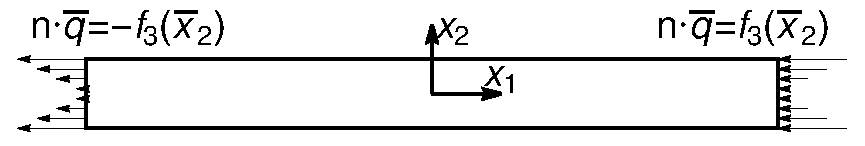
\includegraphics[width=\linewidth]{pics/RectangleFluxF3.pdf} \\ д)
    \end{minipage}
    \hfill
    \begin{minipage}[b][][b]{0.49\linewidth}\centering
        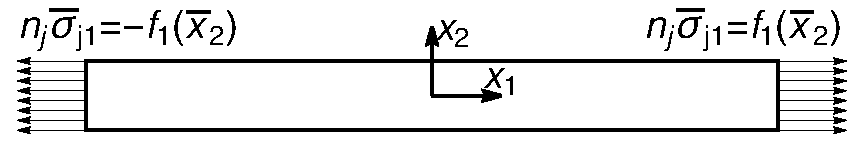
\includegraphics[width=\linewidth]{pics/RectangleStressF1.pdf} \\ б)
        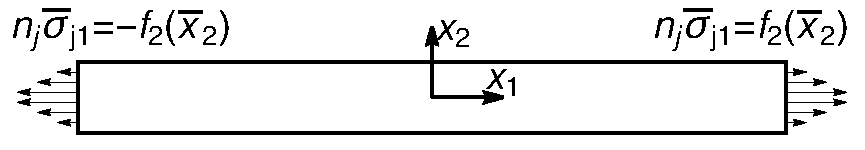
\includegraphics[width=\linewidth]{pics/RectangleStressF2.pdf} \\ г)
        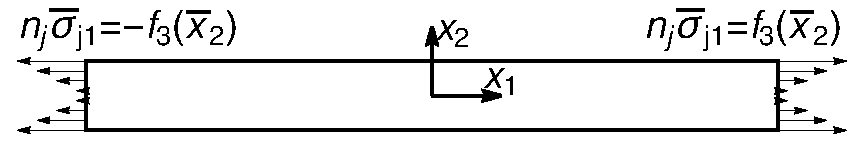
\includegraphics[width=\linewidth]{pics/RectangleStressF3.pdf} \\ е)
    \end{minipage}
    \caption{Тепловые (а, в, д) и механические (б, г, е) нагружения, прикладываемые к пластине на левой и правой границах}
    \label{fig:SaintVenantLoads}
\end{figure}

Вначале рассмотрим распределение компоненты теплового потока $\overline{q}_1$ в локальной и нелокальной постановках. Для этого на Рис.~\ref{fig:FluxStability} рассмотрим сечения $\overline{x}_2 = 0$ и $\overline{x}_2 = 0.5$, где можем увидеть, что несмотря на различные тепловые потоки подведённые к левой и правой границам, при удалении от точек приложения потоки сливаются в единую поверхность, которая в локальном случае является плоскостью $\overline{q}_1 = 1$, а в нелокальном представляет более сложную поверхность.

\begin{figure}[ht]
    \begin{minipage}[b][][b]{0.49\linewidth}\centering
        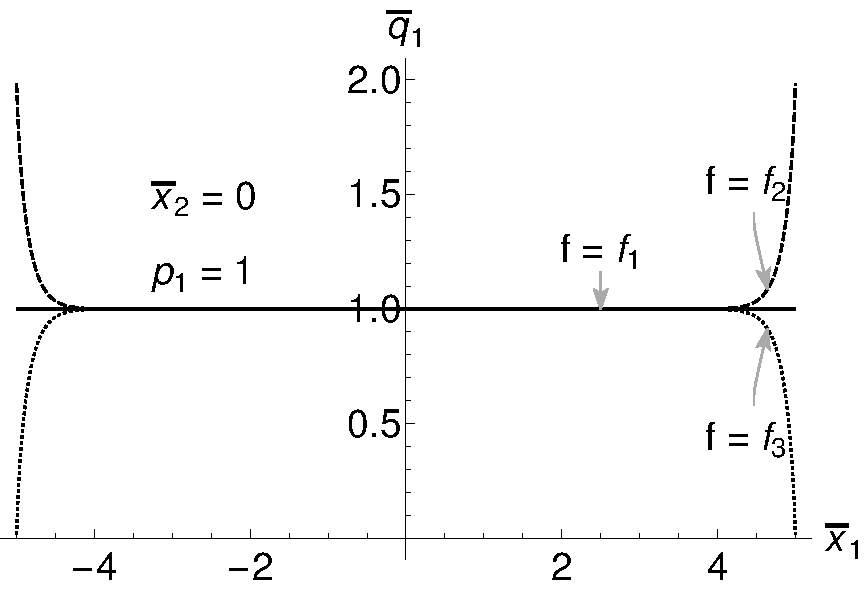
\includegraphics[width=\linewidth]{pics/FluxStabilityX0P1.pdf} \\ а)
        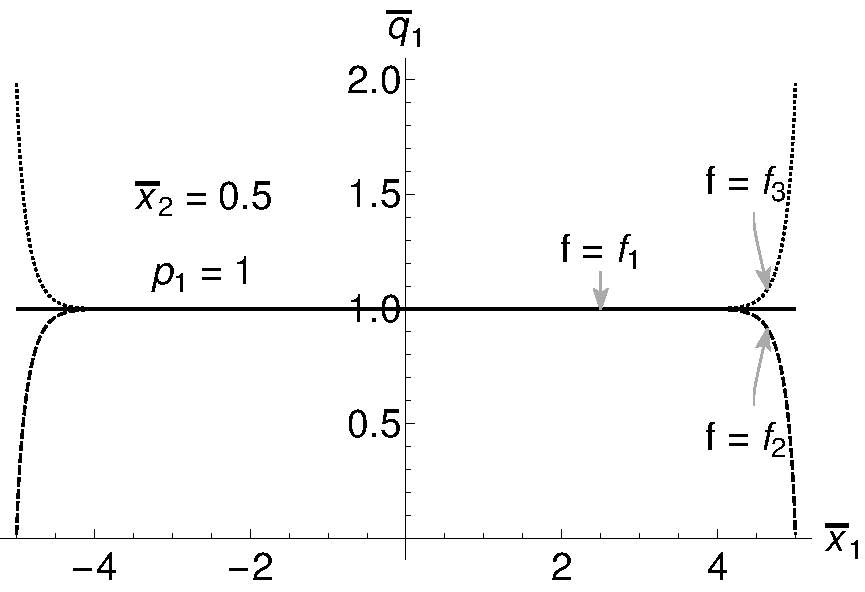
\includegraphics[width=\linewidth]{pics/FluxStabilityX05P1.pdf} \\ в)
    \end{minipage}
    \hfill
    \begin{minipage}[b][][b]{0.49\linewidth}\centering
        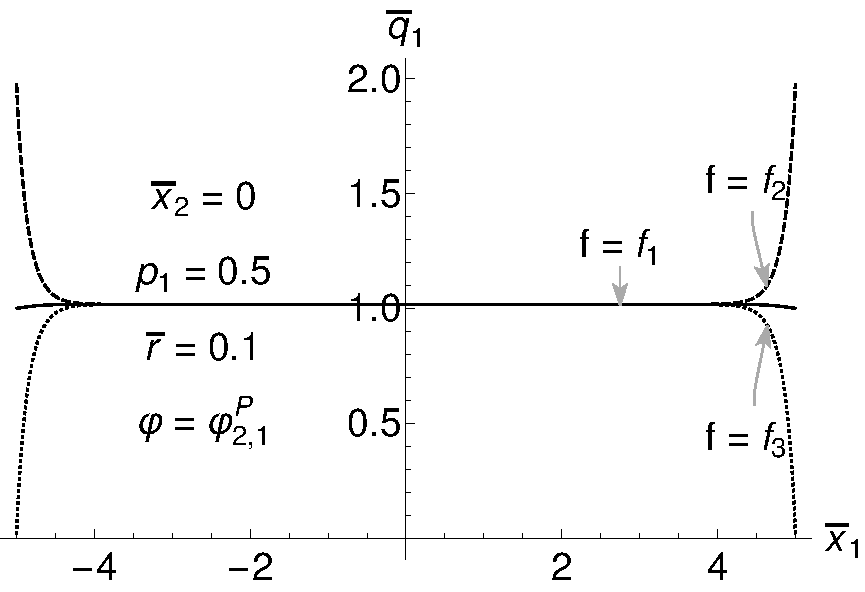
\includegraphics[width=\linewidth]{pics/FluxStabilityX0P05.pdf} \\ б)
        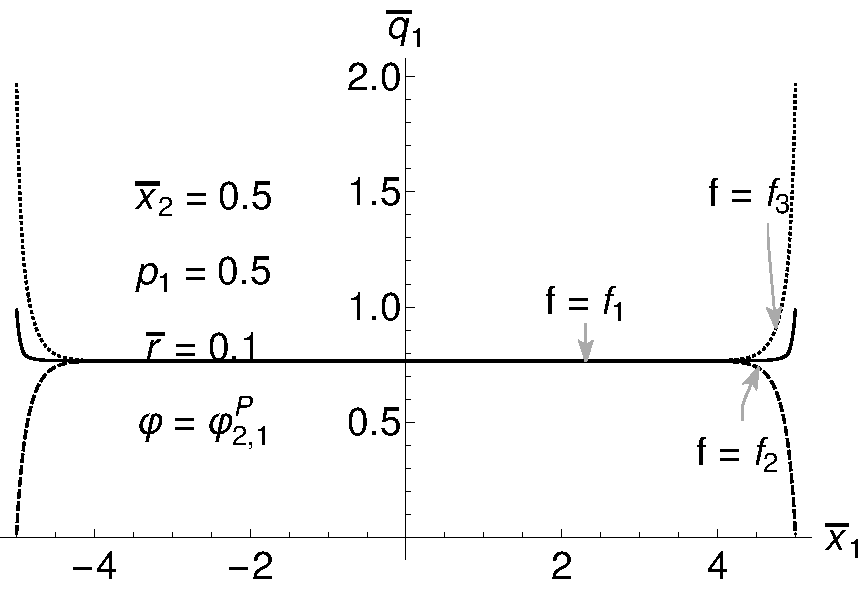
\includegraphics[width=\linewidth]{pics/FluxStabilityX05P05.pdf} \\ г)
    \end{minipage}
    \caption{Распределение компоненты плотности теплового потока $\overline{q}_1$ в сечениях (а, б) $\overline{x}_2 = 0$ и (в, г) $\overline{x}_2 = 0.5$ в (а, в) локальном и (б, г) нелокальном случаях}
    \label{fig:FluxStability}
\end{figure}

Теперь рассмотрим распределение компоненты тензора напряжений $\overline{\sigma}_{11}$. Здесь аналогично ранее рассмотренной компоненте плотности теплового потока $\overline{q}_1$ решения сливаются в общую поверхность, которая, как и в предыдущем случае, в локальной постановке является плоскостью $\overline{\sigma}_{11} = 1$, а в нелокальной представляет некоторую поверхность. На Рис.~\ref{fig:SaintVenant} представлены распределения компоненты тензора напряжений $\overline{\sigma}_{11}$ в сечениях $\overline{x}_2 = 0$ и $\overline{x}_2 = 0.5$ в локальной и нелокальной постановках.

\begin{figure}[ht]
    \begin{minipage}[b][][b]{0.49\linewidth}\centering
        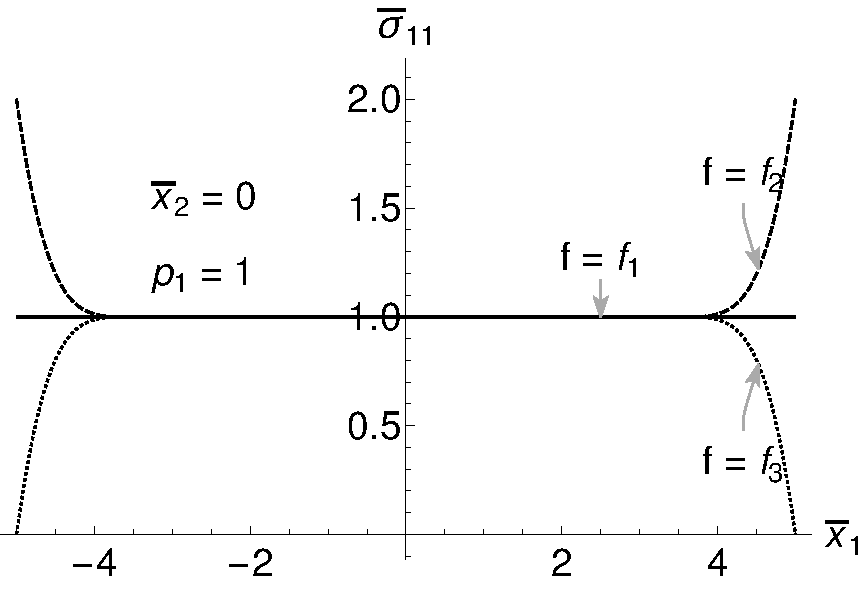
\includegraphics[width=\linewidth]{pics/SaintVenantX0P1.pdf} \\ а)
        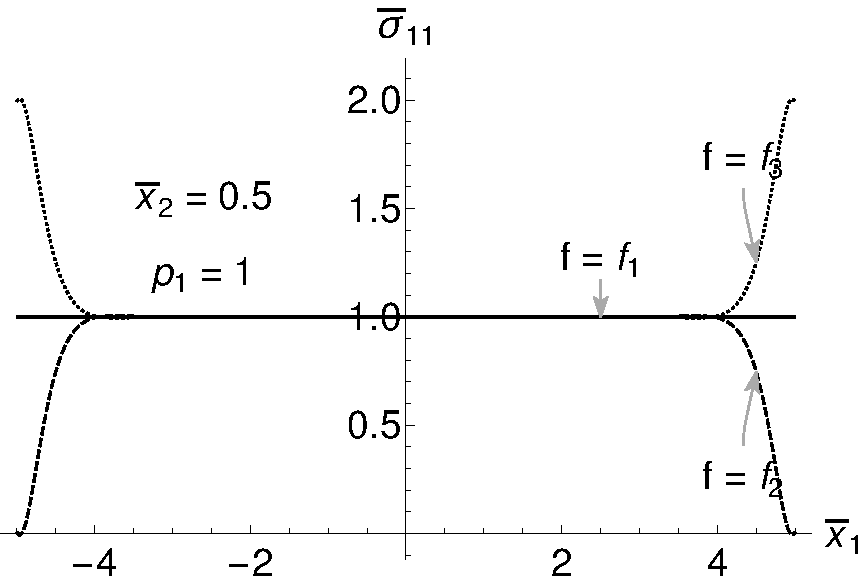
\includegraphics[width=\linewidth]{pics/SaintVenantX05P1.pdf} \\ в)
    \end{minipage}
    \hfill
    \begin{minipage}[b][][b]{0.49\linewidth}\centering
        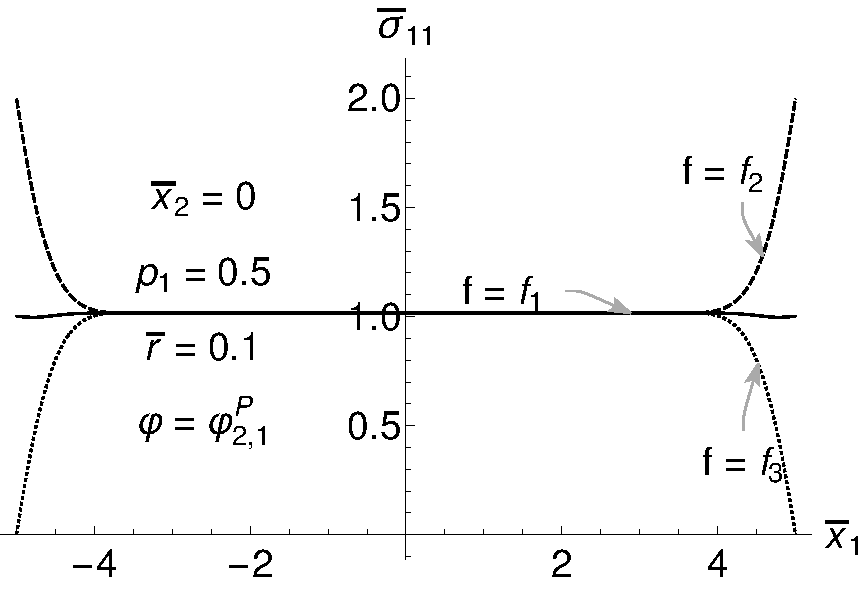
\includegraphics[width=\linewidth]{pics/SaintVenantX0P05.pdf} \\ б)
        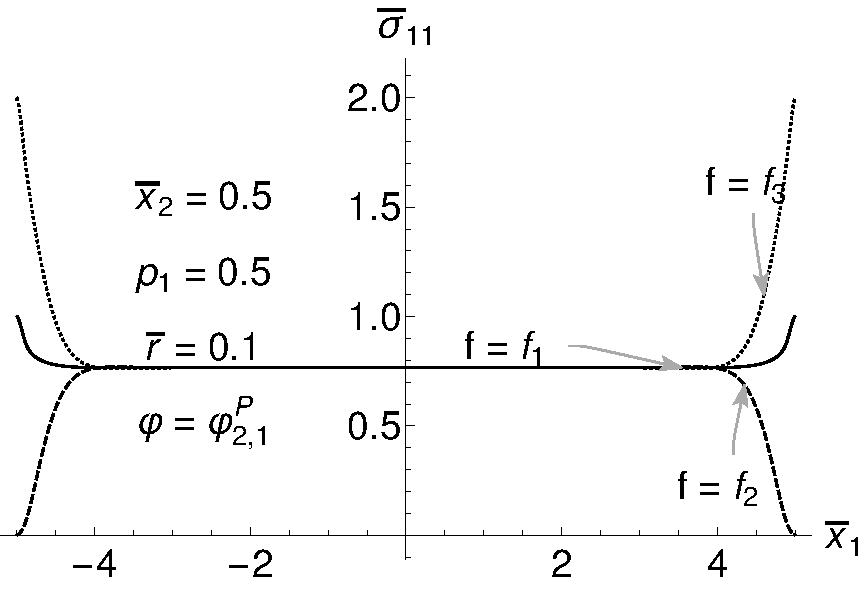
\includegraphics[width=\linewidth]{pics/SaintVenantX05P05.pdf} \\ г)
    \end{minipage}
    \caption{Распределение компоненты тензора напряжений $\overline{\sigma}_{11}$ в сечениях (а, б) $\overline{x}_2 = 0$ и (в, г) $\overline{x}_2 = 0.5$ в (а, в) локальном и (б, г) нелокальном случаях}
    \label{fig:SaintVenant}
\end{figure}

Рис.~\ref{fig:FluxStability} и \ref{fig:SaintVenant} имеют похожие кривые, однако, стабилизация теплового потока происходит заметно быстрее стабилизации напряжений. Для иллюстрации на Рис.~\ref{fig:StabilityLog10} представим логарифмическую разницу решений полученных при нагружениях с использованием функций $f_1$ и $f_2$, где для обобщения обозначений по оси ординат решения будем обозначать символами  $\mathcal{S}_1$ и $\mathcal{S}_2$ соответственно. В полученных распределениях локальные и нелокальные решения имеют одинаковый характер сходимости, но в центре области расхождения между ними начинают возрастать, причём в случае тепловых потоков разница достигает около двух порядков, однако, учитывая порядок величин, такое расхождение можно связать с погрешностями вычислений. Также стоит отметить, что стабилизация теплового потока происходит монотонно, в то время как стабилизация напряжений имеет осцилирующий характер. Это можно понять по изломам графика, то есть в этих точках происходит пересечение кривых.

\begin{figure}[ht]
    \begin{minipage}[b][][b]{0.49\linewidth}\centering
        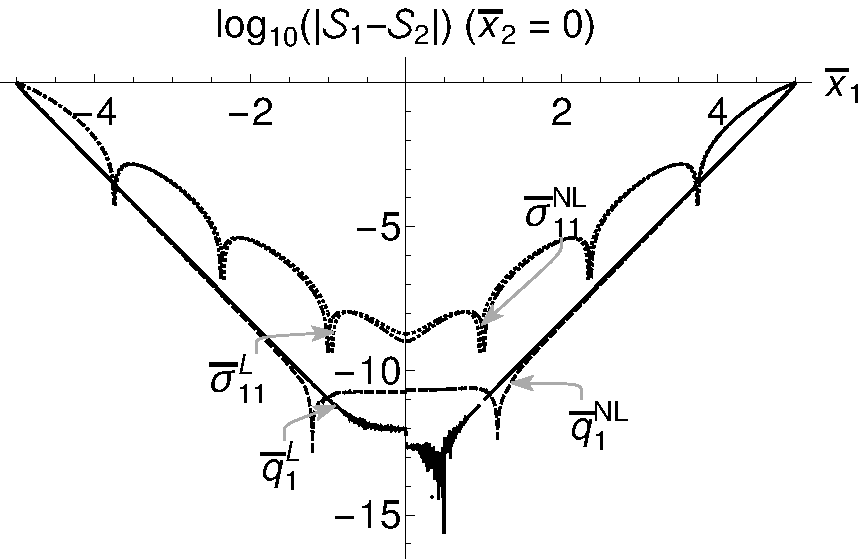
\includegraphics[width=\linewidth]{pics/StabilityLogX0.pdf} \\ а)
    \end{minipage}
    \hfill
    \begin{minipage}[b][][b]{0.49\linewidth}\centering
        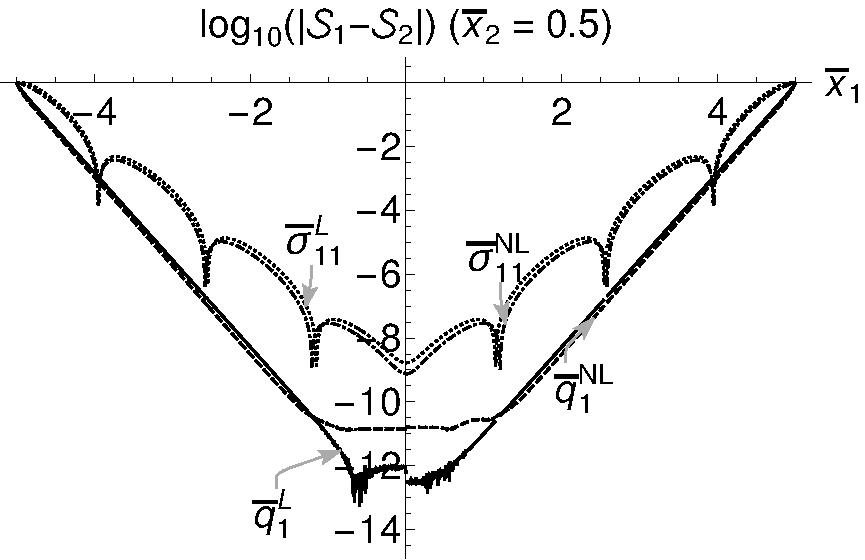
\includegraphics[width=\linewidth]{pics/StabilityLogX05.pdf} \\ б)
    \end{minipage}
    \caption{Логарифмическая разность решений при различных нагружениях в сечениях (a) $\overline{x}_2 = 0$ и (б) $\overline{x}_2 = 0.5$}
    \label{fig:StabilityLog10}
\end{figure}

Теперь рассмотрим сечение вдоль оси $\text{O}\overline{x}_2$. В этом сечении решения обладают кромочным эффектом, который проявляется в снижении уровня рассматриваемой величины на свободных границах области и компенсирующим это снижение повышении этой величины в центре. Вариация радиуса нелокального влияния $\overline{r}$ увеличивает размах кромочного эффекта, а вариация весового параметра $p_1$ влияет на величину отклонения. При этом заметим, что при фиксированном радиусе нелокальности $\overline{r}$ все решения, при различных значениях параметра $p_1$, пересекаются в общих точках. В силу того, что графики компоненты теплового потока $\overline{q}_1$ и компоненты напряжений $\overline{\sigma}_{11}$ в этом сечении не отличаются, изобразим их на общем Рис.~\ref{fig:SaintVenantVariation}, указав по оси ординат обобщающий их символ $\mathcal{S}$.

\begin{figure}[ht]
    \begin{minipage}[b][][b]{0.49\linewidth}\centering
        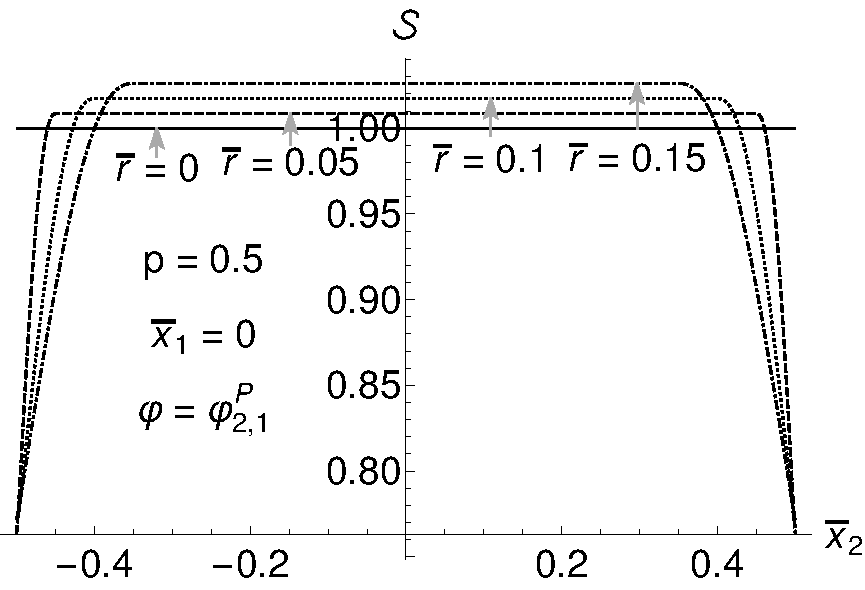
\includegraphics[width=\linewidth]{pics/HeatFluxStabilityVariationR.pdf} \\ а)
    \end{minipage}
    \hfill
    \begin{minipage}[b][][b]{0.49\linewidth}\centering
        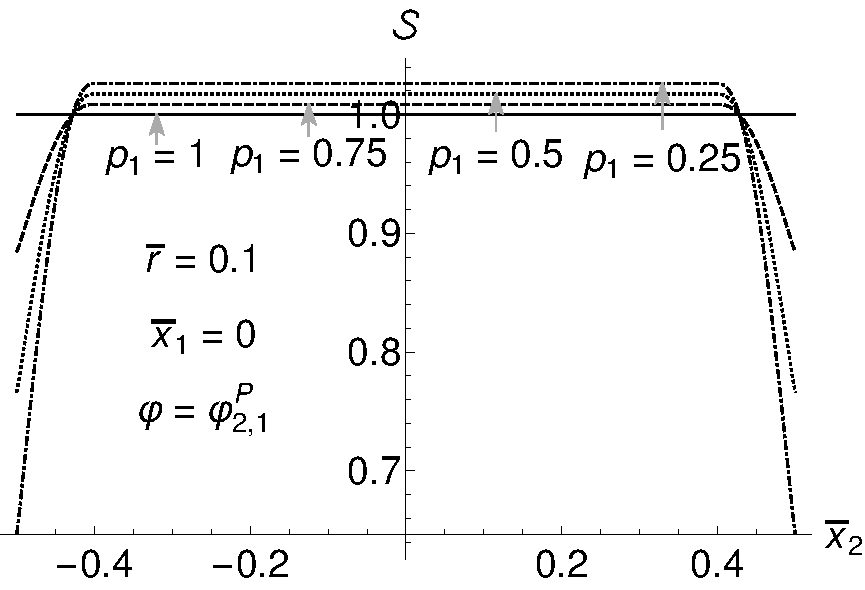
\includegraphics[width=\linewidth]{pics/HeatFluxStabilityVariationP1.pdf} \\ б)
    \end{minipage}
    \caption{Распределение компоненты теплового потока $\overline{q}_1$ и компоненты тензора напряжений $\overline{\sigma}_{11}$ в сечении $\overline{x}_1 = 0$ при вариации (а) $\overline{r}$ и (б) $p_1$}
    \label{fig:SaintVenantVariation}
\end{figure}

Во всех сечениях равнодействующие компоненты теплового потока $\overline{q}_1$ и напряжения $\overline{\sigma}_{11}$ сохраняются и равны приложенным нагружениям:
\begin{gather*}
	\int\limits_{-0.5}^{0.5} \overline{q}_1 d\overline{x}_2 = 
	\int\limits_{-0.5}^{0.5} f_i (\overline{x}_2) d\overline{x}_2,
	\quad
	\int\limits_{-0.5}^{0.5} \overline{\sigma}_{11} d\overline{x}_2 = 
	\int\limits_{-0.5}^{0.5} f_i (\overline{x}_2) d\overline{x}_2,
	\quad	
	i = \overline{1,3}.
\end{gather*}
Это свидетельствует о выполнении принципов стабильности теплового потока и Сен-Венана, а также сохранении балансных соотношений.

\section{Растяжение пластины со ступенчатым переходом}\label{sec:ResultsAnalysis/TShape}

Большой интерес представляет поведение модели на областях с сингулярными точками, где решения стремятся к бесконечности при дроблении сетки. К таким областям относятся области со ступенчатыми переходами, часто возникающими в различных конструкциях и деталях. Для изучения особенностей будет достаточно одного перехода, поэтому рассмотрим простейшую Т-образную область $S$ заключённую в единичный квадрат $\overline{S} = \left\{ \boldsymbol{x} \ | \ 0 \leqslant x_1, x_2 \leqslant 1 \right\}$. Приложим следующие граничные и геометрические условия
\begin{gather*}
	n_j \overline{\sigma}_{j2} |_{\overline{x}_2 = 0} = -1,
	\quad
	\overline{u}_2 |_{\overline{x}_2 = 1} = 0,
	\quad
	\overline{u}_1 |_{\overline{x}_1 = 0.5} = 0.
\end{gather*}
Область с происллюстрированными граничными условиями и интересующими сечениями AB, CD, EF и GH представлена на Рис.~\ref{fig:TArea}. Решение будем искать на равномерной сетке $S_h$ с характерным размером элементов $h = 1/300$.

\begin{figure}[ht]
    \centerfloat{
        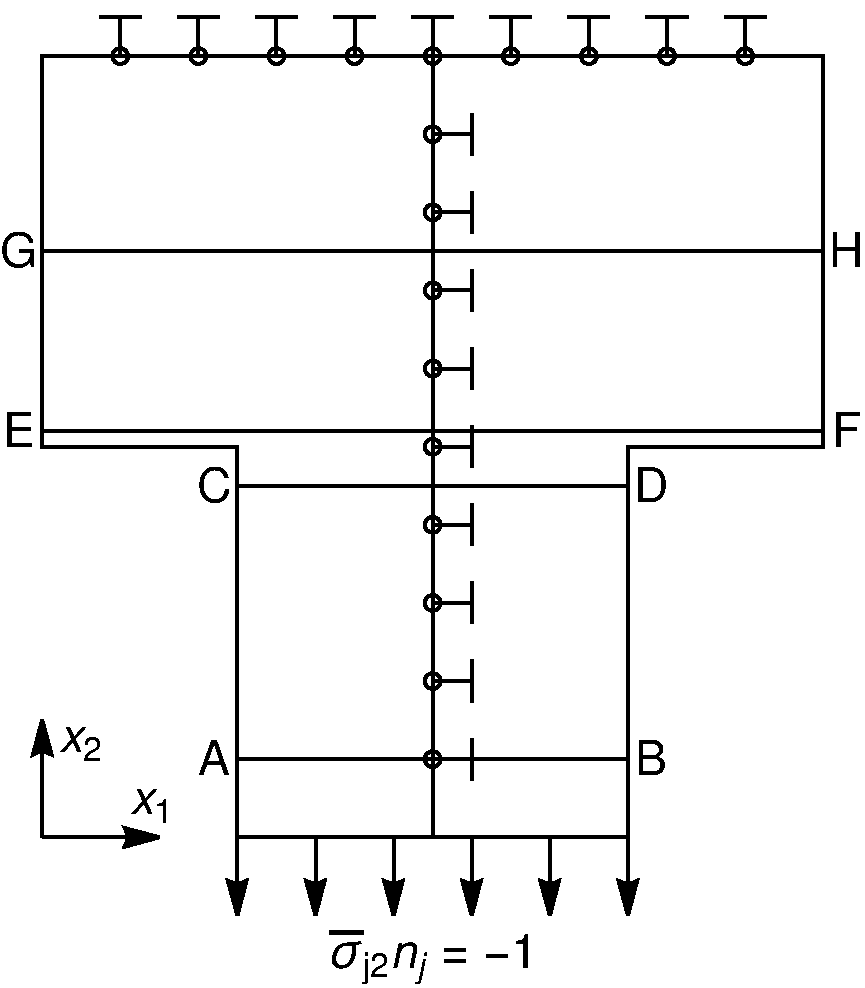
\includegraphics[width=0.5\textwidth]{pics/TArea.pdf}
    }
    \caption{Т-образная область с приложенной нагрузкой}
    \label{fig:TArea}
\end{figure}

Распределение полей компоненты деформации $\varepsilon_{22}$ в локальном и нелокальном случаях при различных радиусах нелокального влияния $\overline{r}$ представлены на Рис.~\ref{fig:TEpsilon}. В нелокальном случае линии уровня изменяют свой характер вблизи границ области, особенно в области ступенчатого перехода, где помимо прочих искажений наблюдаем увеличение деформаций, причём как положительных, так и отрицательных. Линии уровня в областях с отрицательной деформацией становятся более выраженными и их размах увеличивается вместе с радиусом нелокальности $\overline{r}$. В отличие от классического случая, в нелокальном в точках приложения нагружения поле деформации $\varepsilon_{22}$ неравномерно, несмотря на равномерный характер нагружения. Это характеризуется повышенными значениями деформации в углах кромки, к которой приложена нагрузка. Вблизи точек закрепления линии уровня терпят излом, характеризующийся резкой сменой направления линии, которая по итогу, в отличие от классического случая, выходит на границу области не под прямым углом. Крутизна излома уменьшается при увеличении радиуса нелокальности, а расстояние от границы до излома увеличивается.

\begin{figure}[ht]
    \begin{minipage}[b][][b]{0.49\linewidth}\centering
        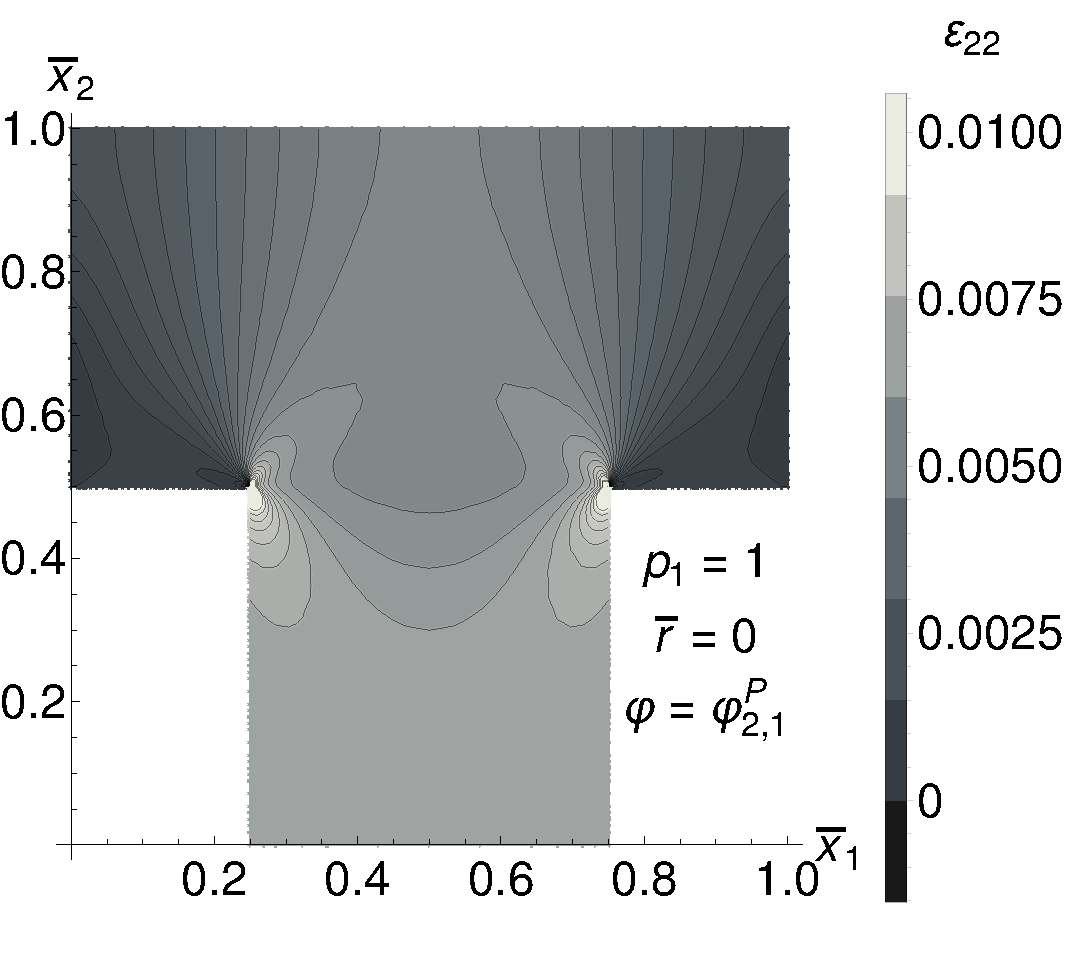
\includegraphics[width=\linewidth]{pics/TEpsR0.pdf} \\ а)
        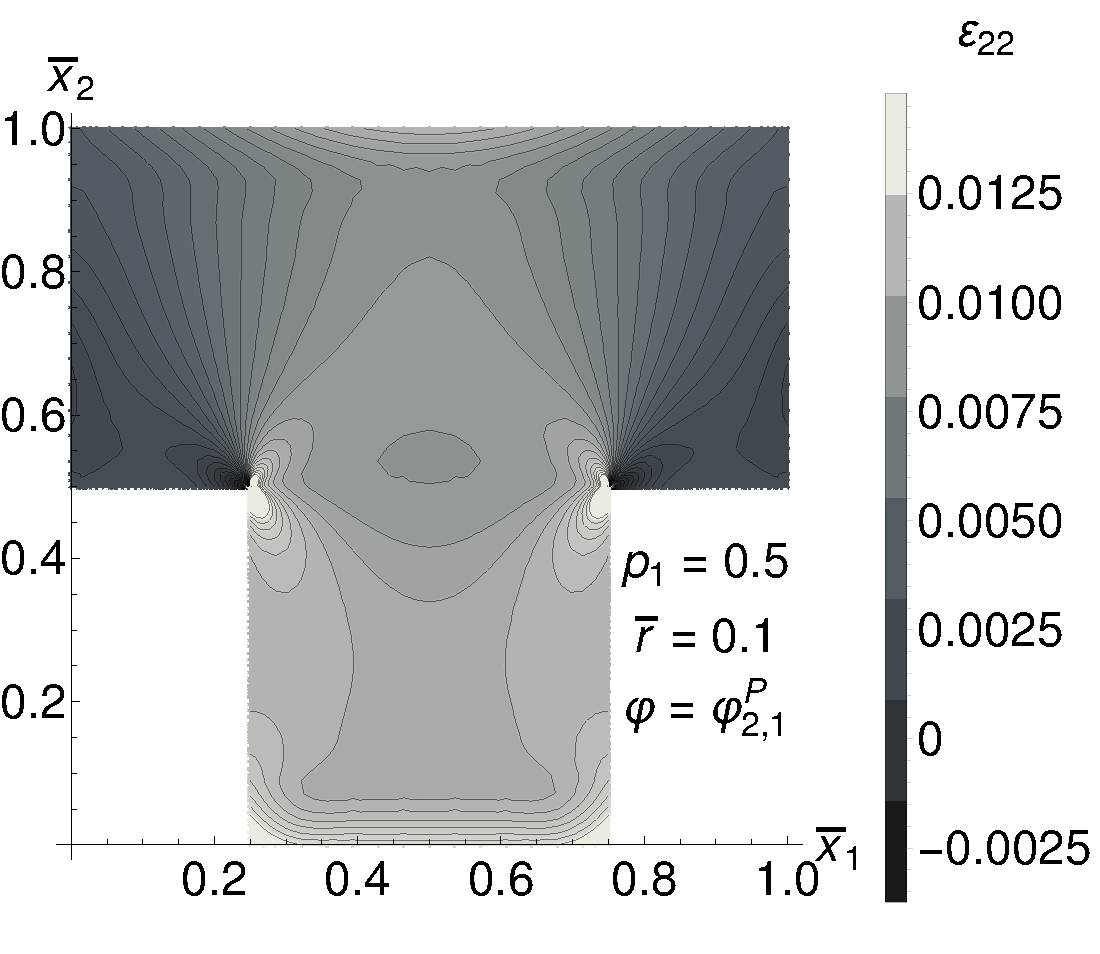
\includegraphics[width=\linewidth]{pics/TEpsR01.pdf} \\ в)
    \end{minipage}
    \hfill
    \begin{minipage}[b][][b]{0.49\linewidth}\centering
        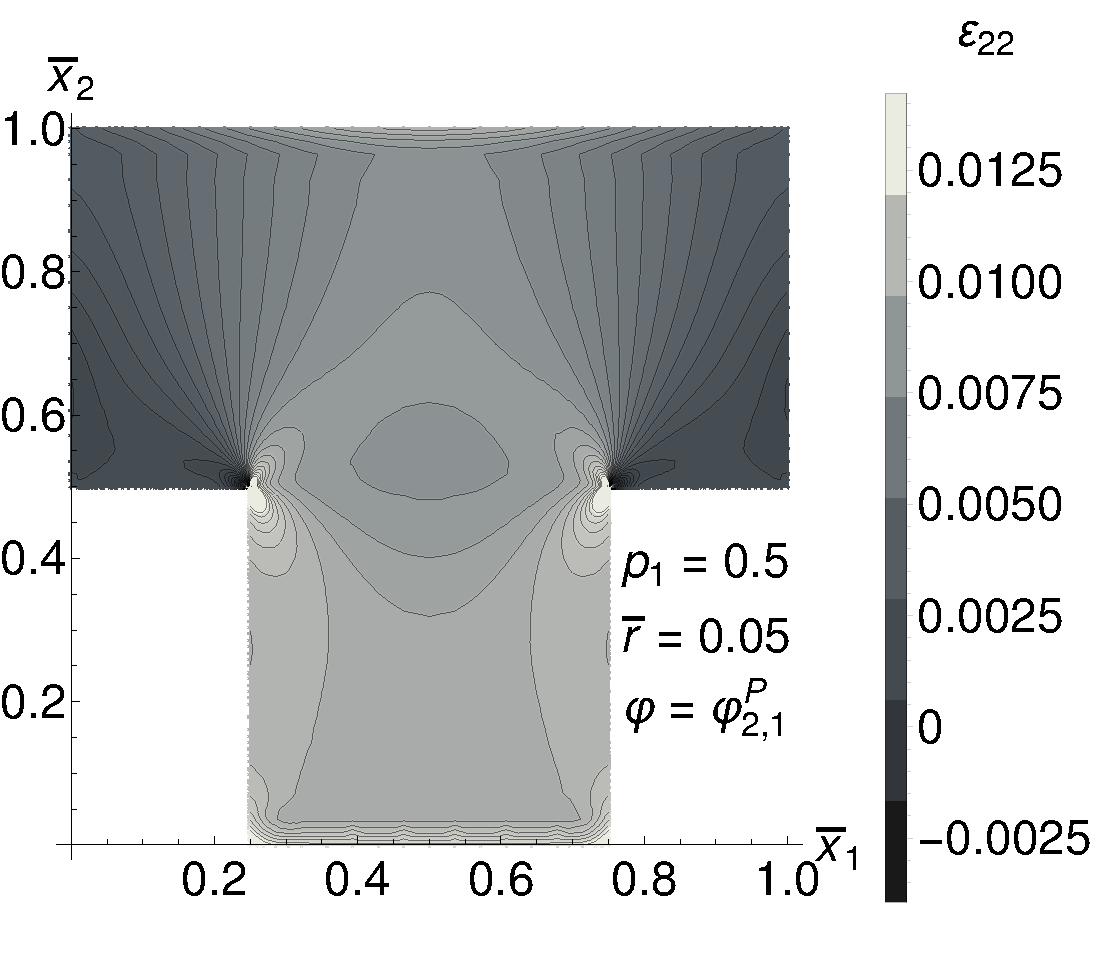
\includegraphics[width=\linewidth]{pics/TEpsR005.pdf} \\ б)
        \includegraphics[width=\linewidth]{pics/TEpsR015.pdf} \\ г)
    \end{minipage}
    \caption{Распределение компоненты тензора деформации $\varepsilon_{22}$ при различных радиусах нелокальности $\overline{r}$}
    \label{fig:TEpsilon}
\end{figure}

Аналогичные распределения деформации в областях со ступенчатыми переходами были получены в результате серии экспериментов под руководством А.В.~Андреева с точным измерением деформаций на пластинах из оптически активных материалов \cite{Andreev}. Деформации измерялись в различных сечениях пластины с использованием 120 тензородатчиков с одинковым механическим сопротивлением. Также был использован альтернативный метод измерения деформации с использованием оптических приборов, где при помощи нанесённой на пластину сетки измерялись перемещения её узлов. При помощи закона Гука и экспериментальных данных о деформациях были определены напряжения и найдены их равнодействующие в сечениях. В работе А.В.~Андреева было показано, что на участке, отстоящем от ступенчатого перехода примерно на четверть ширины ступени, наблюдались наиболее резкие изменения полей деформации и напряжений. Кроме того, в результате экспериментов было установлено, что равнодействующая напряжений, расчитанная по формуле
\begin{gather*}
	\overline{\sigma}_{22}^* = \int\limits_{l_1}^{l_2} \overline{\sigma}_{22} d \overline{x}_1,
\end{gather*}
в сечениях, достаточно удалённых от ступенчатого перехода, равна приложенной нагрузке, а результирующие напряжения в сечениях близких к ступенчатому переходу, оказались в среднем на 30\% меньше приложенного нагружения. Эффект сохранялся при различных значениях нагрузки, а также при двух предельных формах закона Гука, соответствующих плоскому деформированному и плоскому напряжённому состояниям. Объяснением подобного эффекта в работе А.В. Андреева вероятно является тот факт, что классическая теория упругости при расчёте напряжений не позволяет учесть структурных особенностей материала, что и привело к неправильной интерпретации полученных данных.
% Структурная анизотропия???

Действительно, если подставить значения деформации, представленные на Рис.~\ref{fig:TEpsilon}, в классический закон Гука, то получим результаты похожие на те, что были описаны в эксперименте. Распределения результирующего напряжения $\overline{\sigma}_{22}^*$, представленные на Рис.~\ref{fig:ResultantStress22}, также демонстрируют некоторое снижение напряжения сразу после ступенчатого перехода, но не на 30\%, как это было описано в экспериментах. В нижней части области ситуация обратная, результирующее напряжение выше приложенной нагрузки, а в области стыковки двух частей области наблюдаем резкий перепад напряжений. Максимум отклонения находится на нижней и верхней границах области. Отметим, что наибольший вклад на величину отклонения влизи границ области оказывает весовой параметр $p_1$, а на величину отклонения внутри области, а также на ширину отклонения, радиус нелокального влияния $\overline{r}$. При расчёте напряжений по формуле (\ref{eq:DuamelNeumann}) равнодействующая напряжений во всех сечениях равна постоянной, интегрально совпадающей с приложенной нагрузкой.

\begin{figure}[ht]
    \begin{minipage}[b][][b]{0.49\linewidth}\centering
        \includegraphics[width=\linewidth]{pics/ResultantStressVariationR.pdf} \\ а)
    \end{minipage}
    \hfill
    \begin{minipage}[b][][b]{0.49\linewidth}\centering
        \includegraphics[width=\linewidth]{pics/ResultantStressVariationP1.pdf} \\ б)
    \end{minipage}
    \caption{Равнодействующая напряжения $\overline{\sigma}_{22}^*$ при вариации (а) $\overline{r}$ и (б) $p_1$}
    \label{fig:ResultantStress22}
\end{figure}

На Рис.~\ref{fig:TSigma} представлены распределения компоненты напряжения $\overline{\sigma}_{22}$ в сечениях, указанных на Рис.~\ref{fig:TArea}, при различных весовых параметрах $p_1$ и фиксированном радиусе нелокального влияния $\overline{r} = 0.1$. Во всех сечениях увеличение вклада нелокального влияния увеличивает отклонение решения относительно классического. При этом в нижней части области отклонения гораздо более заметные, чем в верхней. Как и в задаче о растяжении прямоугольной пластины, на примере которой ранее был рассмотрен принцип Сен-Венана, здесь наблюдаем существенное снижение напряжения $\overline{\sigma}_{22}$ на свободных от условий границах области. Внутри области напротив происходит повышение уровня напряжений. Отдельно стоит отметить сечение AB, в котором у нелокальных решений образуются <<горбы>> отстоящие на радиус нелокальсти $\overline{r}$ от границ. В сечениях близких к концентратору CD и EF наблюдаем существенное снижение максимального уровня напряжений. А в сечении EF различия в решениях не настолько существенные, как в других сечениях, но также подчиняются всем ранее описанным особенностям. Дополнительно отметим, что при фиксированном радиусе нелокального влияния $\overline{r}$ все решения пересекаются в общих точках.

\begin{figure}[ht]
    \begin{minipage}[b][][b]{0.49\linewidth}\centering
        \includegraphics[width=\linewidth]{pics/TStressAB.pdf} \\ а)
        \includegraphics[width=\linewidth]{pics/TStressEF.pdf} \\ в)
    \end{minipage}
    \hfill
    \begin{minipage}[b][][b]{0.49\linewidth}\centering
        \includegraphics[width=\linewidth]{pics/TStressCD.pdf} \\ б)
        \includegraphics[width=\linewidth]{pics/TStressGH.pdf} \\ г)
    \end{minipage}
    \caption{Распределение напряжений $\overline{\sigma}_{22}$ при различных весовых параметрах $p_1$}
    \label{fig:TSigma}
\end{figure}

\section{Задача Кирша с обобщением на эллиптические вырезы}\label{sec:ResultsAnalysis/KirshProblem}

Продолжим изучение модели на примере решения задачи Кирша с обобщением на эллиптические вырезы. Для этого рассмотрим область $S$, заключённую в квадратную область $\overline{S} = \left\{ \boldsymbol{\overline{x}} \ | \ -1 \leqslant \overline{x}_1, \overline{x}_2 \leqslant 1 \right\}$, с эллиптическим вырезом по центру, где главные оси выреза сонаправлены с осями координат и имеют длины $R_1$ и $R_2$ соответственно. Поставим граничные и геометрические условия
\begin{gather*}
	n_j \overline{\sigma}_{j1} |_{\overline{x}_1 = -1} = -1,
	\quad
	n_j \overline{\sigma}_{j1} |_{\overline{x}_1 = 1} = 1,
	\quad
	\overline{u}_1 |_{\overline{x}_1 = 0} = 0,
	\quad
	\overline{u}_2 |_{\overline{x}_2 = 0} = 0.
\end{gather*}
Схематичное представление области и приложенных нагружений представлены на Рис.~\ref{fig:KirshProblem}, где также введена дополнительная угловая координата $\theta$, необходимая для анализа распределения интересуемых величин на кромке AB. Решение будем искать на структурированной сетке $S_h$, построенной при помощи программного комплекса Abaqus \cite{Abaqus}, пример которой при $R_1 = 0.2$ и $R_2 = 0.4$ с характерным размером элементов $h = 0.05$ представлен на Рис.~\ref{fig:KirshMesh}. Расчёты представленные далее были проведены на более подробных сетках с характерным размером элементов $h = 0.005$ при различных параметра $R_1$ и $R_2$ не превышающих 0.1.

\begin{figure}[ht]
    \centerfloat{
        \includegraphics[width=0.7\textwidth]{pics/EllipseStress.pdf}
    }
    \caption{Постановка задачи Кирша}
    \label{fig:KirshProblem}
\end{figure}

\begin{figure}[ht]
    \centerfloat{
        \includegraphics[width=0.7\textwidth]{pics/KirshMesh.pdf}
    }
    \caption{Пример конечно-элементной сетки на области с эллиптическим вырезом}
    \label{fig:KirshMesh}
\end{figure}

Наибольший интерес исследования представляет распределение деформации и напряжений на кромке эллиптического выреза, но так как задача обладает симметрией, сократим рассматриваемую область до дуги AB. Для удобства исследования введём угловой параметр $\theta$, относительно которого параметризуем координаты дуги следующим образом
\begin{gather*}
	\begin{cases}
		x_1 (\theta) = R_1 \cos \theta, \\
		x_2 (\theta) = R_2 \sin \theta,
	\end{cases}
\end{gather*}
где угол $\theta$ принимает значения от 0 до $\pi / 2$. Затем вычислим длину дуги $l$ с зависимостью от угла $\theta$
\begin{gather*}
	l (\theta) = \int\limits_0^{\theta} \sqrt{
		\left( \dfrac{\partial x_1}{\partial \varphi} \right)^2 +
		\left( \dfrac{\partial x_2}{\partial \varphi} \right)^2
	} d \varphi
\end{gather*}
и наконец обезразмерим этот параметр
\begin{gather}
	\label{eq:NaturalParameter}
	\overline{l} (\theta) = \dfrac{l (\theta)}{l \left( \dfrac{\pi}{2} \right)}.
\end{gather}
Дальнейшие результаты на кромке AB будем рассматривать в координатах безразмерного параметра длины $\overline{l}$. В расчётах будем варьировать отношение длин полуосей выреза таким образом, чтобы максимальная длина была равна 0.1, т.е. $\max(R_1, R_2) = 0.1$. Также для дальнейшего анализа введём величину отношения длин полуосей $\rho = R_2 / R_1$.

Для данной постановки задачи известно, что максимальные значения компоненты тензора напряжений $\overline{\sigma}_{11}^{\max}$ находятся в верхней и нижней точках эллипса и образуют линейную зависимость относительно отношения длин полуосей и прикладываемого нагружения \cite{Birger, Bezuh}
\begin{gather*}
	\overline{\sigma}_{11}^{\max} = \left( 1 + 2 \rho \right) \sigma_0,
\end{gather*}
где $\sigma_0$ --- величина прикладываемой нагрузки. Однако в нелокальном случае максимальный уровень напряжения снижается и начинает зависеть ещё и от весового параметра $p_1$. Рассмотрим результаты представленные в \mbox{Таб. \ref{tab:MaxStress}}, где выписаны значения $\overline{\sigma}_{11}^{\max}$ при различных соотношениях длин полуосей эллипса $R_1$ и $R_2$ и весового параметра $p_1$. Заметим, что данные в локальном случае ($p_1 = 1$) хорошо согласуются с представленной выше зависимостью, а в нелокальном необходимо добавить дополнительный множитель $\kappa$, зависящий от весового параметра $p_1$,
\begin{gather*}
	\overline{\sigma}_{11}^{\max} = \kappa \left( 1 + 2 \rho \right) \sigma_0.
\end{gather*}
Такая зависимость не имеет строгого теоретического доказательства и получена эвристически, однако, она может быть полезна для оценки максимальных значений напряжений в практических расчётах. Для оценки параметра $\kappa$ при фиксированном значеним $p_1$ необходимо провести $n$ расчётов при различных соотношениях длин полуосей и выполнить осреднение согласно следующей формуле
\begin{gather}
	\label{eq:Averaging}
	\kappa (p_1) = \dfrac{1}{n} \sum\limits_{i = 0}^{n} \dfrac{\overline{\sigma}_{11}^{\max} (\rho_i, p_1)}{\overline{\sigma}_{11}^{\max} (\rho_i, 1)},
\end{gather}
где $\rho_i$ --- отношение длин полуосей в $i$-ом расчёте. По результатам, представленным в Таб. \ref{tab:MaxStress}, значения $\kappa$ линейно зависят от весового параметра~$p_1$.

\begin{table}[htbp]
    \centering
    \begin{threeparttable}% выравнивание подписи по границам таблицы
        \caption{Максимальный уровень напряжения $\overline{\sigma}_{11}$ при вариации отношения длин полуосей $\rho$ и весового параметра $p_1$, где $\overline{r} = 0.05$}\label{tab:MaxStress}%
        \begin{tabular}{|c|c|c|c|c|}
	        \hline
			Отношение длин    & \multicolumn{4}{c|}{Весовые параметры} \\
			\cline{2-5}
			полуосей $\rho$   & $p_1 = 1$ & $p_1 = 0.75$ & $p_1 = 0.5$ & $p_1 = 0.25$ \\
			\hline
			$0.5$             & 2.012     & 1.783        & 1.537       & 1.510 \\
			\hline
			$0.75$            & 2.578     & 2.235        & 1.919       & 1.727 \\
			\hline
			$1$               & 3.053     & 2.696        & 2.308       & 1.937 \\
			\hline
			$1.25$            & 3.532     & 3.123        & 2.670       & 2.139 \\
			\hline
			$1.5$             & 4.012     & 3.551        & 3.031       & 2.404 \\
			\hline
			$\kappa$          & 1         & 0.881        & 0.755       & 0.652 \\
			\hline
        \end{tabular}
    \end{threeparttable}
\end{table}

Согласно результатам из Таб. \ref{tab:MaxStress}, при $p_1 = 0.75$ и $p_1 = 0.5$ осреднение (\ref{eq:Averaging}) не нужно, так как результаты отношений напряжений в локальном и нелокальном случаях близки при любых значениях $\rho$, представленных в таблице, но при $p_1 = 0.25$ такая зависимость нарушается, однако, при осреднении зависимость параметра $\kappa$ от весового параметра $p_1$ становится близкой к линейной. Разумеется все эти рассуждения требуют более детального теоретического рассмотрения, так как имеющихся эмпирических данных недостаточно для утверждения явных зависимостей.

Вместе с напряжением $\overline{\sigma}_{11}$, при увеличении значения $\rho$, увеличивается и максимальный уровень деформации $\varepsilon_{11}$. Причём если обратить внимание на Рис.~\ref{fig:EpsABLocAndNonloc} то можем заметить, что помимо повышения максимального уровня деформации она также становится более сконцентрированной в верхней и соответственно нижней точках выреза. В нелокальном случае наблюдаем похожий эффект, однако, здесь также появляется область с отрицательными значениями деформации, которая находится рядом с концентратором. Такой же эффект можно наблюдать при решении нелокальных задач на других областях с концентраторами \cite{ZAMM} и \mbox{экспериментах \cite{Andreev}.}

\begin{figure}[ht]
    \begin{minipage}[b][][b]{0.49\linewidth}\centering
        \includegraphics[width=\linewidth]{pics/KirshABEps11Local.pdf} \\ а)
    \end{minipage}
    \hfill
    \begin{minipage}[b][][b]{0.49\linewidth}\centering
        \includegraphics[width=\linewidth]{pics/KirshABEps11r005p05.pdf} \\ б)
    \end{minipage}
    \caption{Распределение компоненты деформации $\varepsilon_{11}$ на кромке AB в (а) локальном и (б) нелокальном случаях при различных соотношениях длин полуосей выреза}
    \label{fig:EpsABLocAndNonloc}
\end{figure}

При уменьшении параметра $p_1$, в отличие от напряжения $\overline{\sigma}_{11}$, деформация $\varepsilon_{11}$ увеличивается в зоне концентрации. Также увеличивается и смежная с ней зона с отрицательными значениями деформации, а сами значения в ней увеличиваются по модулю. Увеличение радиуса нелокального влияния $\overline{r}$ оказывает похожий  но менее выраженный эффект. Результаты представлены на Рис.~\ref{fig:EpsABVarP1AndR}. В дополнение отметим лишь, что вариация $\overline{r}$ практически не оказывает влияния на величину максимального значения напряжения $\overline{\sigma}_{11}$.

\begin{figure}[ht]
    \begin{minipage}[b][][b]{0.49\linewidth}\centering
        \includegraphics[width=\linewidth]{pics/KirshABEps11VariationP1.pdf} \\ а)
    \end{minipage}
    \hfill
    \begin{minipage}[b][][b]{0.49\linewidth}\centering
        \includegraphics[width=\linewidth]{pics/KirshABEps11VariationR.pdf} \\ б)
    \end{minipage}
    \caption{Распределение компоненты деформации $\varepsilon_{11}$ на кромке AB при вариации (а) весовопого параметра $p_1$ и (б) радиуса нелокальности $\overline{r}$}
    \label{fig:EpsABVarP1AndR}
\end{figure}

\section{Тепловые деформации в областях с эллиптическими вырезами}\label{sec:ResultsAnalysis/ThermalKirshProblem}

Рассмотрим задачу на той же области, что и задачу Кирша, но сменим тип нагружений с механических на тепловые, то есть поставим следующие граничные и геометрические условия
\begin{gather*}
	\boldsymbol{n} \cdot \overline{\boldsymbol{q}}|_{\overline{x}_1 = -1} = 1,
	\quad
	\boldsymbol{n} \cdot \overline{\boldsymbol{q}}|_{\overline{x}_1 = 1} = -1,
	\quad
	\overline{u}_2 |_{\overline{x}_1 = 0} = 0.
\end{gather*}
Графическое изображение постановки задачи представлено на Рис. \ref{fig:ThermalKirshProblem}. Также, для достижения единственности решения, добавим интегральные условия на искомую температуру и первую компоненту вектора перемещения
\begin{gather*}
	\iint\limits_S \overline{T} dS = 0,
	\quad
	\iint\limits_S \overline{u}_1 dS = 0.
\end{gather*}
Такая постановка удобна тем, что позволяет качественно изучить поведение температурных напряжений без появления дополнительных напряжений со стороны возможных концентраторов, обусловленных граничными или геометрическими условиями.

\begin{figure}[ht]
    \centerfloat{
        \includegraphics[width=0.7\textwidth]{pics/EllipseThermal.pdf}
    }
    \caption{Постановка задачи с тепловыми нагружениями}
    \label{fig:ThermalKirshProblem}
\end{figure}

Перед изучением полей напряжений обратим внимание, что аналогично компоненте тензора напряжения $\overline{\sigma}_{11}$ максимальные значения компоненты плотности теплового потока $\overline{q}_1^{\max}$ находятся на верхней и нижней точках эллиптического выреза и они подчинены следующей закономерности
\begin{gather*}
	\overline{q}_1^{\max} = (1 + \rho) q_o,
\end{gather*}
где $q_0$ --- величина подаваемого теплового потока. В нелокальном случае аналогично напряжениям величина $\overline{q}_1^{\max}$ снижается при увеличении вклада нелокального влияния, однако, по результатам представленным в Таб. \ref{tab:MaxFlux} не удаётся также легко определить получившуюся зависимость от $p_1$, так как при весах $p_1 = 0.5$ и $p_1 = 0.25$ и значении $\rho \leqslant 1$ величины $\overline{q}_1^{\max}$ достаточно близки и линейная зависимость от $p_1$ наблюдается только при $\rho = 1.5$.

\begin{table}[htbp]
    \centering
    \begin{threeparttable}% выравнивание подписи по границам таблицы
        \caption{Максимальное значение компоненты теплового потока $\overline{q}_{1}$ при вариации отношения длин полуосей $\rho$ и весового параметра $p_1$, где $\overline{r} = 0.05$}\label{tab:MaxFlux}
        \begin{tabular}{|c|c|c|c|c|}
			\hline
			Отношение длин    & \multicolumn{4}{c|}{Весовые параметры} \\
			\cline{2-5}
			полуосей $\rho$   & $p_1 = 1$ & $p_1 = 0.75$ & $p_1 = 0.5$ & $p_1 = 0.25$ \\
			\hline
			$0.5$             & 1.501     & 1.333        & 1.316       & 1.326 \\
			\hline
			$0.75$            & 1.753     & 1.556        & 1.457       & 1.462  \\
			\hline
			$1$               & 2.001     & 1.781        & 1.597       & 1.591 \\
			\hline
			$1.25$            & 2.252     & 2.002        & 1.734       & 1.644 \\
			\hline
			$1.5$             & 2.494     & 2.222        & 1.927       & 1.681 \\
			\hline
        \end{tabular}
    \end{threeparttable}
\end{table}

Рассмотрим теперь температурные напряжения. Благодаря интегральным условиям, решения получились симметричными и все напряжения сконцентрированы вокруг выреза. Относительно верхней и нижней половин области функции решений чётные, а относительно левой и правой половин нечётные. Зная эти особенности, ограничимся изучением распределения полей напряжения лишь на кромке AB. Для удобства изучения также воспользуемся обезразмеренным параметром длины $\overline{l}$ (\ref{eq:NaturalParameter}).

При вариации параметра $\rho$ кривые $\overline{\sigma}_{11}$ и $\overline{\sigma}_{22}$ существенно изменяют свои формы. На Рис. \ref{fig:ThermalKirshLocal} представлены распределения этих кривых при различных параметрах $\rho$ в классическом случае ($p_1 = 1$). У кривой $\overline{\sigma}_{11}$ вместе с увеличением $\rho$ пиковое значение смещается право вдоль оси O$\overline{l}$. Помимо этого оно также растёт в абсолютных значениях. Максимальная величина $\overline{\sigma}_{22}$ также меняется, но основная закономерность заключается в увеличении площади под кривой при росте $\rho$. Важно отметить, что для обеих кривых в точке $\overline{l} = 1$ их величины равны 0, так как в ней происходит смена знака.

\begin{figure}[ht]
    \begin{minipage}[b][][b]{0.49\linewidth}\centering
        \includegraphics[width=\linewidth]{pics/ThermalKirshSigma11Local.pdf} \\ а)
    \end{minipage}
    \hfill
    \begin{minipage}[b][][b]{0.49\linewidth}\centering
        \includegraphics[width=\linewidth]{pics/ThermalKirshSigma22Local.pdf} \\ б)
    \end{minipage}
    \caption{Распределение напряжения (a) $\overline{\sigma}_{11}$ и (б) $\overline{\sigma}_{22}$ на кромке AB при вариации соотношения длин полуосей}
    \label{fig:ThermalKirshLocal}
\end{figure}

Другими словами, сужение эллиптического выреза вдоль оси O$\overline{x}_1$ приводит к смещению пиковых значений компоненты напряжений $\overline{\sigma}_{11}$ к верхней и нижней точкам выреза, а также увеличению их абсолютных значений. Пиковое значение компоненты напряжений $\overline{\sigma}_{22}$ напротив уменьшается, но при этом занимаемые площади с ненулевыми напряжениями увеличиваются. Таким образом, эллиптические вырезы большая ось которых располагается вдоль линии тока теплового потока дают меньшие напряжения, чем тем, у которых большая ось располагается поперёк.

Учёт нелокальных свойств среды приводит к снижению напряжений $\overline{\sigma}_{11}$ и $\overline{\sigma}_{22}$. Как и во всех расчётах до этого, вариация параметра $\overline{r}$ влияет лишь на форму распределения полей напряжений, а вариация весового параметра $p_1$ на величину отклонения. Распределение полей $\overline{\sigma}_{11}$ и $\overline{\sigma}_{22}$ вдоль кривой AB при вариации $p_1$ представлено на Рис. \ref{fig:ThermalKirshP1Variation}.

\begin{figure}[ht]
    \begin{minipage}[b][][b]{0.49\linewidth}\centering
        \includegraphics[width=\linewidth]{pics/ThermalKirshSigma11VariationP1.pdf} \\ а)
    \end{minipage}
    \hfill
    \begin{minipage}[b][][b]{0.49\linewidth}\centering
        \includegraphics[width=\linewidth]{pics/ThermalKirshSigma22VariationP1.pdf} \\ б)
    \end{minipage}
    \caption{Распределение напряжения (a) $\overline{\sigma}_{11}$ и (б) $\overline{\sigma}_{22}$ на кромке AB при вариации весового параметра $p_1$}
    \label{fig:ThermalKirshP1Variation}
\end{figure}
\chapter{Анализ эффективности программного комплекса NonLocFEM}\label{ch:NonLocFEMAnalysis} 

\section{Тестирование алгоритма ассемблирования матриц}\label{sec:NumericalMethods/AssemblyTest}

Оценим масштабируемость полученного алгоритма ассемблирования матриц теплопроводности и жёсткости (\ref{eq:ApproxNonlocParallel}). Для этого проведём серию расчётов на вычислительном кластере, в состав которого входит 6 вычислительных узлов. На каждом узле кластера установлен 18-ядерный процессор Intel Core i9 10980XE и 128 ГБ оперативной памяти DDR4. Будем рассматривать тестовые задачи на прямоугольной области $S = \{ \boldsymbol{x} | -5 \leqslant x_1 \leqslant 5, -0.5 \leqslant x_2 \leqslant 0.5 \}$, с введённой на ней равномерной сеткой $S_h$. Как и в предыдущей главе, все вычисления проведены с использованием квадратичных серендиповых элементов, интегрирование выполнено гауссовыми квадратурами 3-го порядка (9 квадратурных узлов), а в качестве функции нелокального влияния выбрана $\varphi = \varphi_{2,1}^P$, выбор которой также обоснован в предыдущей главе. Хранение разреженных матриц организовано в формате CSR \cite{Pisanetzkiy}, где для хранения индексов использовались 64-битные целые числа, а для хранения коэффициентов числа с плавающей точкой двойной точности. Также была учтена симметрия матрицы, то есть для хранения и вычисления использовалась только верхняя половина \mbox{матрицы.}

Начнём исследование масштабируемости алгоритмов на машинах с общей памятью, то есть задействуем только один узел кластера и технологию параллельного программирования OpenMP. Для этого проведём серию расчётов варьируя разбиение сетки $h$ и радиус нелокальности $r$, который в данном исследовании совпадает с радиусом поиска. Результаты, представленные в Таблице~\ref{tab:OpenMP}, свидетельствуют о том, что для хранения матрицы жёсткости $\widehat{\textbf{K}}_E$ требуется в 4 раза больше оперативной памяти, чем для матрицы теплопроводности $\widehat{\textbf{K}}_T$ на аналогичной сетке, что было ожидаемо, учитывая размерности блоков матриц теплопроводности (\ref{eq:ThermalBlock}) и жёсткости (\ref{eq:StressBlock}). В обоих случаях, темпы роста занимаемой оперативной памяти относительно разбиения сетки линейные в классическом случае и квадратичные в нелокальном. При сравнении времён сборки матриц можем отметить, что в классическом случае время ассемблирования матрицы жёсткости $\widehat{\textbf{K}}_E$ приблизительно в 3 раза дольше, чем матрицы теплопроводности $\widehat{\textbf{K}}_T$, однако, в нелокальном случае эта разница сокращается до 1.2, чего удалось достичь за счёт оптимизации вычислений с использованием блочного подхода в ассемблировании.

\begin{table}[htbp]
    \centering
    \begin{threeparttable}% выравнивание подписи по границам таблицы
        \caption{Требуемая оперативная память и затрачиваемое время при ассемблировании матриц теплопроводности и жёсткости с использованием технологии OpenMP}\label{tab:OpenMP}
        \begin{tabular}{|c|c|c|c|c|c|c|c|}
	\hline
	Количество & Радиус & \multicolumn{2}{c|}{Требуемая}   & \multicolumn{2}{c|}{Время, с} & \multicolumn{2}{c|}{Время, с} \\
	элементов  & поиска & \multicolumn{2}{c|}{оперативная память} & \multicolumn{2}{c|}{1 поток}  & \multicolumn{2}{c|}{18 потоков} \\
	\cline{3-8}
	      &        & $\widehat{\textbf{K}}_T$ & $\widehat{\textbf{K}}_E$ & $\widehat{\textbf{K}}_T$ & $\widehat{\textbf{K}}_E$ & $\widehat{\textbf{K}}_T$ & $\widehat{\textbf{K}}_E$ \\
	\hline
	$400 \times 40$   & 0    & 6.2 Мб  & 23.8 Мб & 0.061 & 0.187 & 0.028 & 0.048 \\
	\hline
	$800 \times 80$   & 0    & 24.5 Мб & 95 Мб   & 0.521 & 1.701 & 0.116 & 0.274 \\
	\hline
	$1600 \times 160$ & 0    & 97.8 Мб & 379 Мб  & 5.17  & 16.76 & 0.705 & 2.366 \\
	\hline
	$400 \times 40$   & 0.05 & 61.4 Мб & 244 Мб  & 14.4  & 17.06 & 1.055 & 1.288 \\
	\hline
	$800 \times 80$   & 0.05 & 548 Мб  & 2.2 Гб  & 157   & 187   & 11.37 & 13.3  \\
	\hline
	$1600 \times 160$ & 0.05 & 5.5 Гб  & 22 Гб   & 1825  & 2166  & 132.9 & 155   \\
	\hline
	$400 \times 40$   & 0.1  & 133 Мб  & 532 Мб  & 38    & 44.9  & 2.68  & 3.26  \\
	\hline
	$800 \times 80$   & 0.1  & 1.34 Мб & 5.4 Гб  & 450   & 529   & 32    & 37.8  \\
	\hline
	$1600 \times 160$ & 0.1  & 17 Гб   & 68 Гб   & 6134  & 7266  & 447   & 521   \\
	\hline
        \end{tabular}
    \end{threeparttable}
\end{table}

Обращаясь к результатам из Таблицы \ref{tab:OpenMP}, можем построить диаграммы эффективности распараллеливания алгоритмов ассемблирования матриц теплопроводности и жёсткости. Исходя из полученных результатов, представленных на Рис. \ref{fig:OMPParallelization}, отметим достаточно хорошую эффективность распараллеливания, которая в нелокальном случае достигает 14 раз при использовании всех 18 ядер процессора. Однако ускорение в классическом случае не такое высокое, что можно объяснить обобщённостью используемых алгоритмов формирования портрета матрицы, которые недостаточно эффективно работают на малых объёмах данных.

\begin{figure}[ht]
    \begin{minipage}[b][][b]{0.49\linewidth}\centering
        \includegraphics[width=\linewidth]{pics/OMPThermal.pdf} \\ а)
    \end{minipage}
    \hfill
    \begin{minipage}[b][][b]{0.49\linewidth}\centering
        \includegraphics[width=\linewidth]{pics/OMPMechanical.pdf} \\ б)
    \end{minipage}
    \caption{Эффективность распараллеливания алгоритма сборки матриц (а)~теплопроводности и (б)~жёсткости при использовании технологии OpenMP}
    \label{fig:OMPParallelization}
\end{figure}

Теперь исследуем масштабируемость алгоритма ассемблирования матриц на примере использования технологии MPI. Здесь сконцентрируем внимание на алгоритме балансировки данных между процессами, так как вопрос хранения матриц в классе нелокальных задач стоит наиболее остро. Для этого будем рассматривать ту же область, но возьмём более подробную сетку $S_h$, состояющую из $3200 \times 320$ элементов. Радиус нелокальности $r$ выберем равным 0.1. С целью исключения дублирования результатов, остановимся на рассмотрении лишь матрицы теплопроводности.

Проведём сравнение двух запусков на 6 вычислительных узлах кластера. Первый запуск осуществим без балансировки данных, то есть распределения узлов сетки между процессами оставим равномерным. Второй запуск осуществим с балансировкой данных между процессами, которая выполняется по алгоритму описанному в третьей главе. На Рис. \ref{fig:MPIBalance} представлены полученные распределения затрачиваемой оперативной памяти для хранения блоков матрицы на каждом узле. В варианте без балансировки данные распределены не равномерно и некоторым узлам кластера достался объём данных больше, чем другим. В варианте с балансировкой данные распределены, в рамках допустимой погрешности, равномерно. Из чего можно сделать вывод, что алгоритм балансировки данных работает корректно.

\begin{figure}[ht]
    \begin{minipage}[b][][b]{0.49\linewidth}\centering
        \includegraphics[width=\linewidth]{pics/PieChartNoBalance.pdf} \\ а)
    \end{minipage}
    \hfill
    \begin{minipage}[b][][b]{0.49\linewidth}\centering
        \includegraphics[width=\linewidth]{pics/PieChartBalance.pdf} \\ б)
    \end{minipage}
    \caption{Распределение размеров блоков матрицы теплопроводности между 6 процессами в случае (а) без балансировки и (б) с балансировкой данных}
    \label{fig:MPIBalance}
\end{figure}

В качестве замечания можно ещё отметить, что алгоритм балансировки данных также ускоряет работу метода сопряжённых градиентов, так как операция умножения матрицы на вектор становится одинаковой по трудозатратам на каждом узле кластера. Более подробно про другие возможные методы ускорения сходимости решателей СЛАУ обсудим в последующих разделах.

\section{Анализ скорости сходимости при оптимизации базиса конечных элементов}\label{sec:NumericalMethods/BasisOptimization}

В работе повсеместно использовались квадратичные серендиповые элементы, в связи с чем возникла потребность оптимизиации их базиса для ускорения сходимости итерационных методов решения СЛАУ. Отметим, что у квадратичного серендипового элемента есть целое параметрическое семейство базисов, представленное в третьей главе диссертации. В той же главе была получена оценка оптимального значения параметра $s$ (\ref{eq:ParamSOptimal}) согласно которой скорость сходимости должна быть максимальной в точке $s = 2/9$. Проверим эту оценку на практике, а заодно исследуем влияние других параметров модели.

Для проверки корректности оценки решим серию задач варьируя параметр $s$. Расчёты снова будем проводить на прямоугольной области $S = \{ \boldsymbol{x} \ | \ -5 \leqslant x_1 \leqslant 5, -0.5 \leqslant x_2 \leqslant 0.5  \}$, с введённой на этой области равномерной сеткой $S_h = 1000 \times 100$. Обезразмерим уравнения (\ref{eq:StationaryHeatEquation}) и (\ref{eq:EquilibriumEquation}) относительно коэффициента теплопроводности $\lambda$ и модуля Юнга $E$ соответственно
\begin{gather*}
	\overline{\boldsymbol{q}} = \dfrac{\boldsymbol{q}}{\lambda},
	\quad
	\overline{\boldsymbol{\sigma}} = \dfrac{\widehat{\boldsymbol{\sigma}}}{E},
\end{gather*}
так как параметры $\lambda$ и $E$ в данном случае выступают в роли масштабирующих множителей для собственных чисел матриц $\widehat{\textbf{K}}_T$ и $\widehat{\textbf{K}}_E$ соответственно. Коэффициент Пуассона $\nu$ примем равным 0.3. Поставим граничные условия для уравнения теплопроводности
\begin{gather*}
	\boldsymbol{n} \cdot \overline{\boldsymbol{q}} |_{x_1 = -5} = -1,
	\quad
	\boldsymbol{n} \cdot \overline{\boldsymbol{q}} |_{x_1 = 5} = 1,
	\quad
	\int\limits_S T dS = 0,
\end{gather*}
и для уравнения равновесия
\begin{gather*}
	n_j \overline{\sigma}_{j1} |_{x_1 = -5} = -1,
	\quad
	n_j \overline{\sigma}_{j1} |_{x_1 = 5} = 1,
	\quad
	u_1 |_{x_1 = 0} = 0,
	\quad
	u_2 |_{x_2 = 0} = 0.
\end{gather*}
Решение СЛАУ будем искать методом сопряжённых градиентов без использования каких-либо дополнительных предобуславливателей.

Для определения числа обусловленности (\ref{eq:CondValue}) необходимо вычислить максильное и минимальное собственные числа матрицы. Для их вычисления к программному комплексу NonLocFEM была подключена библиотека Spectra \cite{SpectraLib}, которая позволяет вычислять собственные числа разреженных матриц и совместима с библиотекой линейной алгебры Eigen \cite{EigenLib}.

В ходе экспериментов было установлено, что минимальное собственное число $\lambda_{\min}$ не зависит от параметра базиса $s$ и вариаций функции нелокальности $\varphi$, но при этом имеет некоторую зависимость от вклада нелокального влияния и радиуса нелокальности $r$, где при их увеличении величина собственного числа $\lambda_{\min}$ начинает уменьшаться. Однако исходя из результатов, представленных в Таблицах \ref{tab:ThermalEigenMin} и \ref{tab:StressEigenMin}, можем сделать вывод, что зависимость от параметров модели весьма слабая, так как величина изменений не достигает и десятой доли от числа полученного в классическом случае, то есть минимальное собственное число не оказывает серьёзного влияния на число обусловленности. Также можно отметить, что минимальные собственные числа матриц теплопроводности и жёсткости при одинаковых параметрах модели достаточно близки по значениям.

\begin{table}[htbp]
    \centering
    \begin{threeparttable}% выравнивание подписи по границам таблицы
        \caption{Зависимость минимального собственного числа матрицы теплопроводности $\widehat{\textbf{K}}_T$ от параметров модели $p_1$ и $r$}\label{tab:ThermalEigenMin}
        \begin{tabular}{|c|c|c|c|c|}
			\hline
			\backslashbox{$r$}{$p_1$} & 1 & 0.75 & 0.5 & 0.25 \\
			\hline
			0    & $3.2637 \cdot 10^{-6}$ & --- & --- & --- \\
			\hline
			0.05 & --- & $3.2429 \cdot 10^{-6}$ & $3.2181 \cdot 10^{-6}$ & $3.1793 \cdot 10^{-6}$ \\
			\hline
			0.1  & --- & $3.2231 \cdot 10^{-6}$ & $3.1750 \cdot 10^{-6}$ & $3.0997 \cdot 10^{-6}$ \\
			\hline
			0.15 & --- & $3.2032 \cdot 10^{-6}$ & $3.1319 \cdot 10^{-6}$ & $3.0218 \cdot 10^{-6}$ \\
			\hline
        \end{tabular}
    \end{threeparttable}
\end{table}

\begin{table}[htbp]
    \centering
    \begin{threeparttable}% выравнивание подписи по границам таблицы
        \caption{Зависимость минимального собственного числа матрицы жёсткости $\widehat{\textbf{K}}_E$ от параметров модели $p_1$ и $r$}\label{tab:StressEigenMin}
        \begin{tabular}{|c|c|c|c|c|}
			\hline
			\backslashbox{$r$}{$p_1$} & 1 & 0.75 & 0.5 & 0.25 \\
			\hline
			0    & $3.2614 \cdot 10^{-6}$ & --- & --- & --- \\
			\hline
			0.05 & --- & $3.2471 \cdot 10^{-6}$ & $3.2328 \cdot 10^{-6}$ & $3.1958 \cdot 10^{-6}$ \\
			\hline
			0.1  & --- & $3.2336 \cdot 10^{-6}$ & $3.1911 \cdot 10^{-6}$ & $3.1191 \cdot 10^{-6}$ \\
			\hline
			0.15 & --- & $3.2183 \cdot 10^{-6}$ & $3.1489 \cdot 10^{-6}$ & $3.0435 \cdot 10^{-6}$ \\
			\hline
        \end{tabular}
    \end{threeparttable}
\end{table}

Максимальные собственные числа $\lambda_{\max}$ матриц теплопроводности $\widehat{\textbf{K}}_T$ и жёсткости $\widehat{\textbf{K}}_E$ напротив имеют достаточно сильную зависимость как от параметра базиса $s$, так и от весового параметра модели $p_1$. При этом зависимость от весового параметра $p_1$ удаётся установить эмпирически, она в точности равна $\lambda_{\max}^{NL}(s) = p_1 \lambda_{\max}^{L}(s)$. Зависимость от радиуса нелокальности $r$ и функции нелокальности $\varphi$ у максимальных собственных чисел отсутствует. Результаты представлены в Таблицах \ref{tab:ThermalIterAndMaxEgien} и \ref{tab:MechanicalIterAndMaxEgien}, где также представлены данные о количествах итераций метода сопряжённых градиентов.

\begin{table}[htbp]
    \centering
    \begin{threeparttable}% выравнивание подписи по границам таблицы
        \caption{Зависимости количества итераций $N$ и максимального собственного числа $\lambda_{\max}$ матрицы теплопроводности $\widehat{\textbf{K}}_T$ от вариации параметров $p_1$ и $s$}\label{tab:ThermalIterAndMaxEgien}
        \begin{tabular}{|c|c|c|c|c|c|c|c|c|}
			\hline
			Значение & \multicolumn{2}{c|}{$p_1 = 1$} & \multicolumn{2}{c|}{$p_1 = 0.75$} & \multicolumn{2}{c|}{$p_1 = 0.5$} & \multicolumn{2}{c|}{$p_1 = 0.25$} \\ 
			\cline{2-9}
			параметра $s$ & $N$  & $\lambda_{\max}$ & $N$  & $\lambda_{\max}$ & $N$  & $\lambda_{\max}$ & $N$  & $\lambda_{\max}$ \\ 
			\hline
			-1/3 & 6961 & 15.997 & 8724 & 11.997 & 5036 & 7.9980 & 3549 & 3.9984 \\
			\hline
			-2/9 & 5600 & 11.198 & 5110 & 8.3986 & 4341 & 5.5987 & 2948 & 2.7990 \\
			\hline
			-1/9 & 4540 & 7.4660 & 4095 & 5.5993 & 3367 & 3.7327 & 2360 & 1.8663 \\
			\hline
			   0 & 3868 & 5.3332 & 3640 & 3.9997 & 2891 & 2.6662 & 1961 & 1.3328 \\
			\hline
			 1/9 & 3885 & 5.3332 & 3442 & 3.9997 & 2861 & 2.6662 & 1947 & 1.3328 \\
			\hline 
			 2/9 & 4000 & 5.3332 & 3600 & 3.9997 & 2826 & 2.6662 & 2003 & 1.3328 \\
			\hline 
			 1/3 & 3889 & 5.3332 & 3567 & 3.9997 & 2778 & 2.6662 & 1948 & 1.3328 \\
			\hline 
			 4/9 & 3786 & 5.3332 & 3474 & 3.9997 & 2835 & 2.6662 & 1982 & 1.3328 \\
			\hline 
			 5/9 & 4719 & 7.4660 & 4415 & 5.5993 & 3525 & 3.7327 & 2353 & 1.8663 \\
			\hline 
			 2/3 & 5761 & 11.198 & 6887 & 8.3986 & 4134 & 5.5987 & 2982 & 2.7990 \\
			\hline 
			 7/9 & 7218 & 15.997 & 6349 & 11.997 & 5285 & 7.9980 & 3720 & 3.9984 \\
			\hline
        \end{tabular}
    \end{threeparttable}
\end{table}

\begin{table}[htbp]
    \centering
    \begin{threeparttable}% выравнивание подписи по границам таблицы
        \caption{Зависимости количества итераций $N$ и максимального собственного числа $\lambda_{\max}$ матрицы жёсткости $\widehat{\textbf{K}}_E$ от вариации параметров $p_1$ и $s$}\label{tab:MechanicalIterAndMaxEgien}
        \begin{tabular}{|c|c|c|c|c|c|c|c|c|}
			\hline
			Значение & \multicolumn{2}{c|}{$p_1 = 1$} & \multicolumn{2}{c|}{$p_1 = 0.75$} & \multicolumn{2}{c|}{$p_1 = 0.5$} & \multicolumn{2}{c|}{$p_1 = 0.25$} \\ 
			\cline{2-9}
			параметра $s$ & $N$  & $\lambda_{\max}$ & $N$  & $\lambda_{\max}$ & $N$  & $\lambda_{\max}$ & $N$  & $\lambda_{\max}$ \\ 
			\hline
			-1/3 & 7454 & 13.061 & 6549 & 9.7954 & 4758 & 6.5298 & 3893 & 3.2650 \\
			\hline
			-2/9 & 6261 & 9.6366 & 5066 & 7.2272 & 4402 & 4.8178 & 3344 & 2.4090 \\
			\hline
			-1/9 & 4805 & 7.0840 & 4820 & 5.3128 & 3992 & 3.5416 & 2870 & 1.7707 \\
			\hline
			   0 & 4797 & 5.4194 & 3996 & 4.0643 & 3053 & 2.7094 & 2509 & 1.3545 \\
			\hline   
			 1/9 & 4380 & 4.5195 & 3320 & 3.3897 & 2703 & 2.2602 & 2289 & 1.1306 \\
			\hline 
			 2/9 & 4272 & 4.2968 & 3296 & 3.2222 & 2727 & 2.1476 & 2229 & 1.0730 \\
			\hline 
			 1/3 & 4270 & 4.2970 & 3551 & 3.2224 & 2641 & 2.1477 & 2229 & 1.0731 \\
			\hline 
			 4/9 & 4085 & 4.3423 & 3772 & 3.2566 & 3124 & 2.1709 & 2242 & 1.0852 \\
			\hline 
			 5/9 & 4446 & 6.1015 & 3911 & 4.5760 & 3704 & 3.0504 & 2659 & 1.5249 \\
			\hline 
			 2/3 & 6138 & 8.8614 & 4814 & 6.6458 & 4464 & 4.4302 & 3203 & 2.2147 \\
			\hline 
			 7/9 & 7076 & 12.436 & 5567 & 9.3273 & 4634 & 6.2178 & 3802 & 3.1083 \\
			\hline
        \end{tabular}
    \end{threeparttable}
\end{table}

Теперь рассмотрим данные из таблиц \ref{tab:ThermalEigenMin}-\ref{tab:MechanicalIterAndMaxEgien} в графическом представлении. На Рис. \ref{fig:ThermalCondAndIter} представлены зависимости числа обсусловленности и количества итераций метода сопряжённых градиентов от параметра базиса $s$ и весового параметра модели $p_1$. Обратим внимание, что кривые числа обусловленности симметричные относительно точки $s = 2/9$, а также, что число обусловленности снижается по мере уменьшения весового параметра $p_1$. Также стоит отметить, что на интервале $0 \leqslant s \leqslant 4/9$ кривые числа обусловленности выходят на плато, центром которого по прежнему является точка $s = 2/9$. Кривые зависимости числа итераций хорошо коррелируют с кривыми числа обусловленности и минимум числа итераций находится в окрестностях точки $s = 2/9$, а увеличение вклада нелокального влияния ускоряет сходимость метода при заданных параметрах.



Результаты, представленные на Рис. \ref{fig:MechanicalCondAndIter}, для матрицы жёсткости аналогичны результатам, представленным на Рис. \ref{fig:ThermalCondAndIter}, для матрицы теплопроводности, однако, здесь графики зависимости числа обусловленности от параметра $s$ уже не являются симметричными и плато на них уже менее выражено, а графики зависимости числа итераций хуже коррелируют с графиками числа обусловленности. Тем ни менее, минимум числа обусловленности и числа итераций по прежнему находится в окрестностях точки $s = 2/9$ из чего можно сделать вывод, что оценка (\ref{eq:ParamSOptimal}) пригодна для практического использования.

Также важно отметить, что несмотря на то, что количество итераций в нелокальном случае становится меньше, время затрачиваемое на решение СЛАУ в нелокальном случае может быть на несколько порядков больше, чем для аналогичной задачи в классическом случае. Это связано с объёмами данных, которые занимают матрицы в нелокальном случае и главным сдерживающим фактором в скорости решения СЛАУ выступает скорость работы оперативной памяти, а не процессора.

\begin{figure}[ht]
    \begin{minipage}[b][][b]{0.49\linewidth}\centering
        \includegraphics[width=\linewidth]{pics/ThermalCond.pdf} \\ а)
    \end{minipage}
    \hfill
    \begin{minipage}[b][][b]{0.49\linewidth}\centering
        \includegraphics[width=\linewidth]{pics/ThermalIter.pdf} \\ б)
    \end{minipage}
    \caption{Зависимость (а) числа обусловленности и (б) количества итераций $N$ для матрицы теплопроводности $\widehat{\textbf{K}}_T$ от параметров $s$ и $p_1$ при $r = 0.1$}
    \label{fig:ThermalCondAndIter}
\end{figure}

\begin{figure}[ht]
    \begin{minipage}[b][][b]{0.49\linewidth}\centering
        \includegraphics[width=\linewidth]{pics/MechanicalCond.pdf} \\ а)
    \end{minipage}
    \hfill
    \begin{minipage}[b][][b]{0.49\linewidth}\centering
        \includegraphics[width=\linewidth]{pics/MechanicalIter.pdf} \\ б)
    \end{minipage}
    \caption{Зависимость (а) числа обусловленности и (б) количества итераций $N$ для матрицы жёсткости $\widehat{\textbf{K}}_E$ от параметров $s$ и $p_1$ при $r = 0.1$}
    \label{fig:MechanicalCondAndIter}
\end{figure}

\section{Предобуславливание и выбор начального приближения}\label{sec:NumericalMethods/Preconditioning}

Оптимизированный базис квадратичных серендиповых элементов позволил ускорить сходимость метода сопряжённых градиентов при решении СЛАУ более чем в 1.5 раза по сравнению со случаем, когда используется классический базис. Однако существует возможность добиться ещё большей скорости сходимости за счёт использования предобуславливателей или более подходящих начальных условий.

При разработке предобуславливателя важно учитывать специфику задачи, так как универсальных способов эффективного предобуславливания не существует. Также важно учитывать возможности современных вычислительных машин: параллельные вычисления зачастую дают заметно больший выигрыш во времени, в отличие от предобуславливания в силу того, что многие популярные методы предобуславливания используют обратный алгоритм Гаусса, который не всегда возможно эффективно распараллелить, а накладные расходы при этом могут значительно увеличить цену одной итерации.

Пожалуй основной спецификой рассматриваемого класса уравнений является их матрично-векторное представление (\ref{eq:ThermalSLAE}) и (\ref{eq:StressSLAE}), где матричные выражения представлены в виде взвешенных сумм локальных $\widehat{\textbf{K}}^L_{\mathcal{F}}$ и нелокальных $\widehat{\textbf{K}}^{NL}_{\mathcal{F}}$ матриц. При этом локальные слагаемые обалают заметно меньшей плотностью заполнения, чем нелокальные. Учитывая эту специфику, а также уже рассмотренный анализ границ спектров матриц $\widehat{\textbf{K}}_{\mathcal{F}}$, можем построить предобуславливатель используя для этого лишь локальное слагаемое.

Как правило для построения предобуславливателей необходимы данные о максимальных и минимальных собственных числах, однако, процесс нахождения границ спектра, даже для локальной матрицы, является слишком медленным. Поэтому примем во внимание полученные знания о связи спектров локальной и полной матриц и в качестве предобуславливателя возьмём неполное разложение Холецкого локальной матрицы $\widehat{\textbf{K}}^L_{\mathcal{F}}$, так как оно не требует непосредственного поиска собственных чисел.

Теперь проведём серию расчётов и на её основе определим эффективность использования предобуславливателя. В этом же исследовании проверим гипотезу о выборе начального приближения, где в качестве начального приближения выберем результат решения СЛАУ $\widehat{\textbf{K}}^L_{\mathcal{F}} \cdot \textbf{X}_0 = \textbf{F}$, где $\textbf{F}$ --- вектор правой части, на основе которого будем решать полную СЛАУ и $\textbf{X}_0$ --- вектор искомого начального приближения. Для теста будем рассматривать задачи из предыдущего раздела, а базис элементов выберем оптимальным с параметром $s = 2/9$.

По результатам, представленным в Таблицах \ref{tab:ThermalPrecond} и \ref{tab:StressPrecond} для уравнений теплопроводности и равновесия соотвественно, можем сделать вывод, что использование предобуславливателя позволяет ускорить решение СЛАУ в N раз. При этом весовые параметры модели на это не оказывают серьёзного влияния. Вместе с этим можно сделать вывод касательно выбора начального приближения. Однако предложенная гипотеза не даёт ожидаемого эффекта, количество итераций сокращается несущественно, а время затрачиваемое на решение СЛАУ для классической задачи не всегда меньше получаемого выигрыша. В качестве замечания стоит добавить, что для краткости записи формулировка в таблице ILLT$\left( \widehat{\textbf{K}}^L_T \right)$ означает использование предобуславливателя, а ILLT$\left( \widehat{\textbf{K}}^L_T \right) + X_0$ подразумевает комбинацию предобуславливания и начального приближения.

\begin{table}[htbp]
    \centering
    \begin{threeparttable}% выравнивание подписи по границам таблицы
        \caption{Количество итераций и затрачиваемое время при решении СЛАУ уравнения теплопроводности}\label{tab:ThermalPrecond}
        \begin{tabular}{|c|c|c|c|c|c|c|}
		\hline
		$p_1$ & \multicolumn{2}{c|}{Без предобуславливания} & \multicolumn{2}{c|}{ILLT$\left( \widehat{\textbf{K}}^L_T \right)$} & \multicolumn{2}{c|}{ILLT$\left( \widehat{\textbf{K}}^L_T \right) + X_0$}\\
		\cline{2-7}
		     & $N$ & $t$, с & $N$ & $t$, с & $N$ & $t$, с \\
		\hline
		0.75 & 5364 & 2970 & 2111 & 1181 & 2086 & 1238 (1167) \\
		\hline
		0.5  & 4558 & 2527 & 1740 & 972 & 1742 & 1045 (974) \\
		\hline
		0.25 & 3020 & 1673 & 1250 & 657 & 1265 & 779 (708) \\
		\hline
        \end{tabular}
    \end{threeparttable}
\end{table}

\begin{table}[htbp]
    \centering
    \begin{threeparttable}% выравнивание подписи по границам таблицы
        \caption{Количество итераций и затрачиваемое время при решении СЛАУ уравнения равновесия}\label{tab:StressPrecond}
        \begin{tabular}{|c|c|c|c|c|c|c|}
		\hline
		$p_1$ & \multicolumn{2}{c|}{Без предобуславливания} & \multicolumn{2}{c|}{ILLT$\left( \widehat{\textbf{K}}^L_T \right)$} & \multicolumn{2}{c|}{ILLT$\left( \widehat{\textbf{K}}^L_T \right) + X_0$}\\
		\cline{2-7}
		     & $N$ & $t$, с & $N$ & $t$, с & $N$ & $t$, с \\
		\hline
		0.75 & 6330 & 13238 & 2902 & 6217 & 2736 & 6223 (5967) \\
		\hline
		0.5  & 5167 & 10811 & 2290 & 4915 & 2389 & 5442 (5203) \\
		\hline
		0.25 & 3779 & 7888 & 1718 & 3695 & 1740 & 4032 (3793) \\
		\hline
        \end{tabular}
    \end{threeparttable}
\end{table}
\chapter*{Общие выводы и заключение}                       % Заголовок
\addcontentsline{toc}{chapter}{Общие выводы и заключение}  % Добавляем его в оглавление

%% Согласно ГОСТ Р 7.0.11-2011:
%% 5.3.3 В заключении диссертации излагают итоги выполненного исследования, рекомендации, перспективы дальнейшей разработки темы.
%% 9.2.3 В заключении автореферата диссертации излагают итоги данного исследования, рекомендации и перспективы дальнейшей разработки темы.
%% Поэтому имеет смысл сделать эту часть общей и загрузить из одного файла в автореферат и в диссертацию:


%% Согласно ГОСТ Р 7.0.11-2011:
%% 5.3.3 В заключении диссертации излагают итоги выполненного исследования, рекомендации, перспективы дальнейшей разработки темы.
%% 9.2.3 В заключении автореферата диссертации излагают итоги данного исследования, рекомендации и перспективы дальнейшей разработки темы.
\begin{enumerate}
	\item Рассмотрена иерархия моделей нелокальной теплопроводности и термоупругости, предложено и проанализировано два семейства возможных функций нелокального влияния, заданных на областях, ограниченных кривыми Ламэ.
	
	\item Разработан численный алгоритм решения интегро-дифференциальных уравнений на основе метода конечных элементов, проведена работа над его оптимизацией и подготовкой к использованию в параллельной среде вычислений.
	
	\item Разработан собственный программный комплекс NonLocFEM, в рамках которого реализованы все предложенные алгоритмы; параллельные реализации алгоритмов задействуют технологии параллельного программирования OpenMP и MPI, все исследования и расчёты проведены в рамках программного комплекса.
	
	\item Проведён качественный анализ сравнения классических теорий теплопроводности и термоупругости с их нелокальными постановками, полученные результаты свидетельствуют о снижении роли концентраторов в распределениях полей напряжений и плотности теплового потока и в возникновении кромочных эффектов на свободных от граничных условий границах, а также определены основные зависимости отклонений нелокальных решений относительно классическим путём вариации параметров модели.
	
	\item Исследован вопрос сходимости итерационных методов решения СЛАУ применительно к задачам в нелокальных постановках, предложены способы ускорения сходимости с применением альтернативных базисов конечных элементов и предобуславливателей.
\end{enumerate}

%И какая-нибудь заключающая фраза.

%Последний параграф может включать благодарности.  В заключение автор
%выражает благодарность и большую признательность научному руководителю
%Иванову~И.\,И. за поддержку, помощь, обсуждение результатов и~научное
%руководство. Также автор благодарит Сидорова~А.\,А. и~Петрова~Б.\,Б.
%за помощь в~работе с~образцами, Рабиновича~В.\,В. за предоставленные
%образцы и~обсуждение результатов, Занудятину~Г.\,Г. и авторов шаблона
%*Russian-Phd-LaTeX-Dissertation-Template* за~помощь в оформлении
%диссертации. Автор также благодарит много разных людей
%и~всех, кто сделал настоящую работу автора возможной.
      % Заключение
\include{Dissertation/acronyms}        % Список сокращений и условных обозначений
\chapter*{Словарь терминов}             % Заголовок
\addcontentsline{toc}{chapter}{Словарь терминов}  % Добавляем его в оглавление

\textbf{СЛАУ} : Система линейных алгебраических уравнений

\textbf{ЭВМ} : Электронная вычислительная машина

\textbf{MPI} : Message Passing Interface

\textbf{OpenMP} : Open Multi-Processing      % Словарь терминов
\include{Dissertation/references}      % Список литературы
%\include{Dissertation/lists}           % Списки таблиц и изображений (иллюстративный материал)

\setcounter{totalchapter}{\value{chapter}} % Подсчёт количества глав

%%% Настройки для приложений
%\appendix
% Оформление заголовков приложений ближе к ГОСТ:
%\setlength{\midchapskip}{20pt}
%\renewcommand*{\afterchapternum}{\par\nobreak\vskip \midchapskip}
%\renewcommand\thechapter{\Asbuk{chapter}} % Чтобы приложения русскими буквами нумеровались

%%\chapter{}\label{app:A}
\chapter*{Приложение} 
\addcontentsline{toc}{chapter}{Приложение}

Ниже представлен Листинг 1 конфигурационного файла, на основе которого был произведён расчёт комбинированной задачи темплопроводности и термоупругости из раздела \ref{sec:ResultsAnalysis/ThermalKirshProblem}. Конфигурационный файл выполнен в виде структуры, описанной в формате JSONSchema, и содержит 6 основных полей: task, save, mesh, thermal\_boundaries, mechanical\_boundaries и materials.

В поле task описаны основные характеристики запускаемой задачи: её размерность, тип расчёта и зависимость расчёта от времени. В поле save содержатся параметры сохранения результатов расчётов, указан путь сохранения результатов, а также названия сохраняемых файлов и точность с которой записывать результаты расчётов. В разделе mesh указан путь по которому находится файл содержащий конечно-элементную сетку. Поля thermal\_boundaries и mechanical\_boundaries содержат граничные условия для температурной и механической задач соответственно. Здесь важно отметить, что граничные условия заданы на именованных границах, поэтому важно, чтобы сетка содержала информацию об этих границах в виде групп элементов. В разделе materials указаны физические параметры материала и модельные параметры отдельно для уравнения теплопроводности и уравнения равновесия. Здесь также важно отметить, что информация о материале задана на именованной группе элементов, которые обозначают определённый материал. Таких групп может быть несколько, где для каждого материала могут быть заданы свои параметры.

\begingroup
\captiondelim{ } % разделитель идентификатора с номером от наименования
\lstinputlisting[lastline=87,language={},caption={Конфигурационный файл для комбинированной задачи теплопроводности и термоупругости},label={lst:external1}]{listings/thermomechanical_2d.json}
\endgroup
        % Приложения

%\setcounter{totalappendix}{\value{chapter}} % Подсчёт количества приложений

\end{document}
